%# -*- coding: utf-8-unix -*-
%%==================================================
%% thesis.tex
%%==================================================

% 双面打印
%\documentclass[doctor, openright, twoside]{sjtuthesis}
% \documentclass[bachelor, openany, oneside, submit]{sjtuthesis}
 \documentclass[master,review]{sjtuthesis}
% \documentclass[%
%   bachelor|master|doctor, % 必选项
%   fontset=fandol|windows|mac|ubuntu|adobe|founder, % 字体选项
%   oneside|twoside,        % 单面打印,双面打印(奇偶页交换页边距,默认)
%   openany|openright,      % 可以在奇数或者偶数页开新章|只在奇数页开新章(默认)
%   english,                % 启用英文模版
%   review,     % 盲审论文,隐去作者姓名、学号、导师姓名、致谢、发表论文和参与的项目
%   submit      % 定稿提交的论文,插入签名扫描版的原创性声明、授权声明 
% ]

% 逐个导入参考文献数据库
\addbibresource{bib/ref.bib}
% \addbibresource{bib/chap2.bib}

%%# -*- coding: utf-8-unix -*-
% !TEX program = xelatex
% !TEX root = ../thesis.tex
% !TEX encoding = UTF-8 Unicode
\title{上海交通大学学位论文 \\ \LaTeX{} 模板示例文档}
\author{某\quad{}某}
\advisor{某某教授}
% \coadvisor{某某教授}
\defenddate{2014年12月17日}
\school{上海交通大学}
\institute{某某系}
\studentnumber{0010900990}
\major{某某专业}
\keywords{上海交大, 饮水思源, 爱国荣校}

\englishtitle{A Sample Document for \LaTeX-basedd SJTU Thesis Template}
\englishauthor{\textsc{Mo Mo}}
\englishadvisor{Prof. \textsc{Mou Mou}}
% \englishcoadvisor{Prof. \textsc{Uom Uom}}
\englishschool{Shanghai Jiao Tong University}
\englishinstitute{\textsc{Depart of XXX, School of XXX} \\
  \textsc{Shanghai Jiao Tong University} \\
  \textsc{Shanghai, P.R.China}}
\englishmajor{A Very Important Major}
\englishdate{Dec. 17th, 2014}
\englishkeywords{SJTU, master thesis, XeTeX/LaTeX template}

  % NOTE: the enclosed commands must be executed in preamble
%# -*- coding: utf-8-unix -*-
% !TEX program = xelatex
% !TEX root = ../thesis.tex
% !TEX encoding = UTF-8 Unicode
\title{基于深度强化学习的对抗性策略研究}
\author{娄欢}
\advisor{李建勋教授}
% \coadvisor{某某教授}
\defenddate{2019年2月18日}
\school{上海交通大学}
\institute{电子信息与电气工程学院}
\studentnumber{116032910070}
\major{控制工程}
\keywords{深度强化学习,数据扩充,GAN,博弈,决策}

\englishtitle{Research on adversarial strategies based on deep reinforcement learning}
\englishauthor{\textsc{Lou Huan}}
\englishadvisor{Prof. \textsc{Li Jianxun}}
% \englishcoadvisor{Prof. \textsc{Uom Uom}}
\englishschool{Shanghai Jiao Tong University}
\englishinstitute{\textsc{Depart of Automation, School of Electronic Information and Electrical Engineering} \\
  \textsc{Shanghai Jiao Tong University} \\
  \textsc{Shanghai, P.R.China}}
\englishmajor{Control Engineering}
\englishdate{Feb. 18th, 2019}
\englishkeywords{Deep reinforcement learning,Data augmentation,GAN,Game,Decision }
\begin{document}

% 无编号内容:中英文论文封面、授权页
\maketitle

\makeatletter
\ifsjtu@submit\relax
  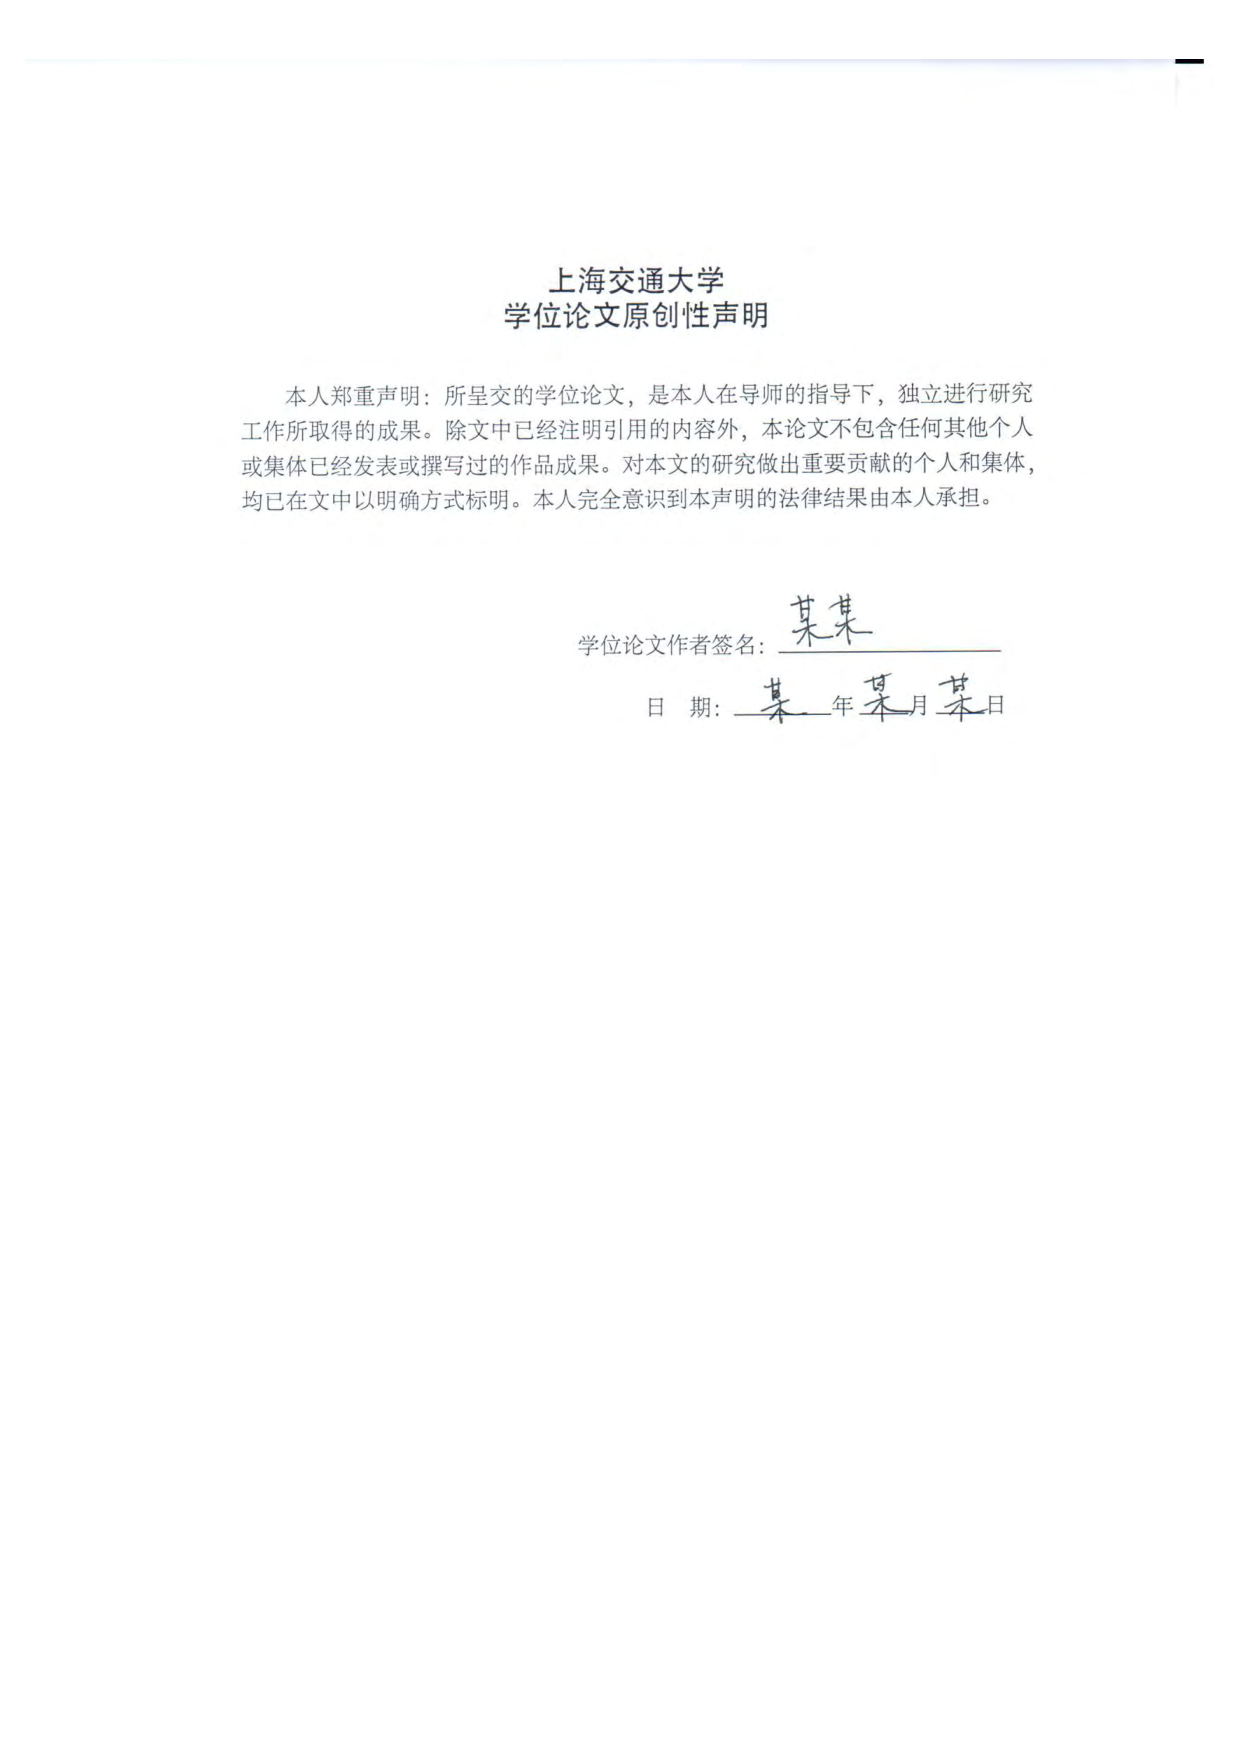
\includepdf{pdf/original.pdf}
  \cleardoublepage
  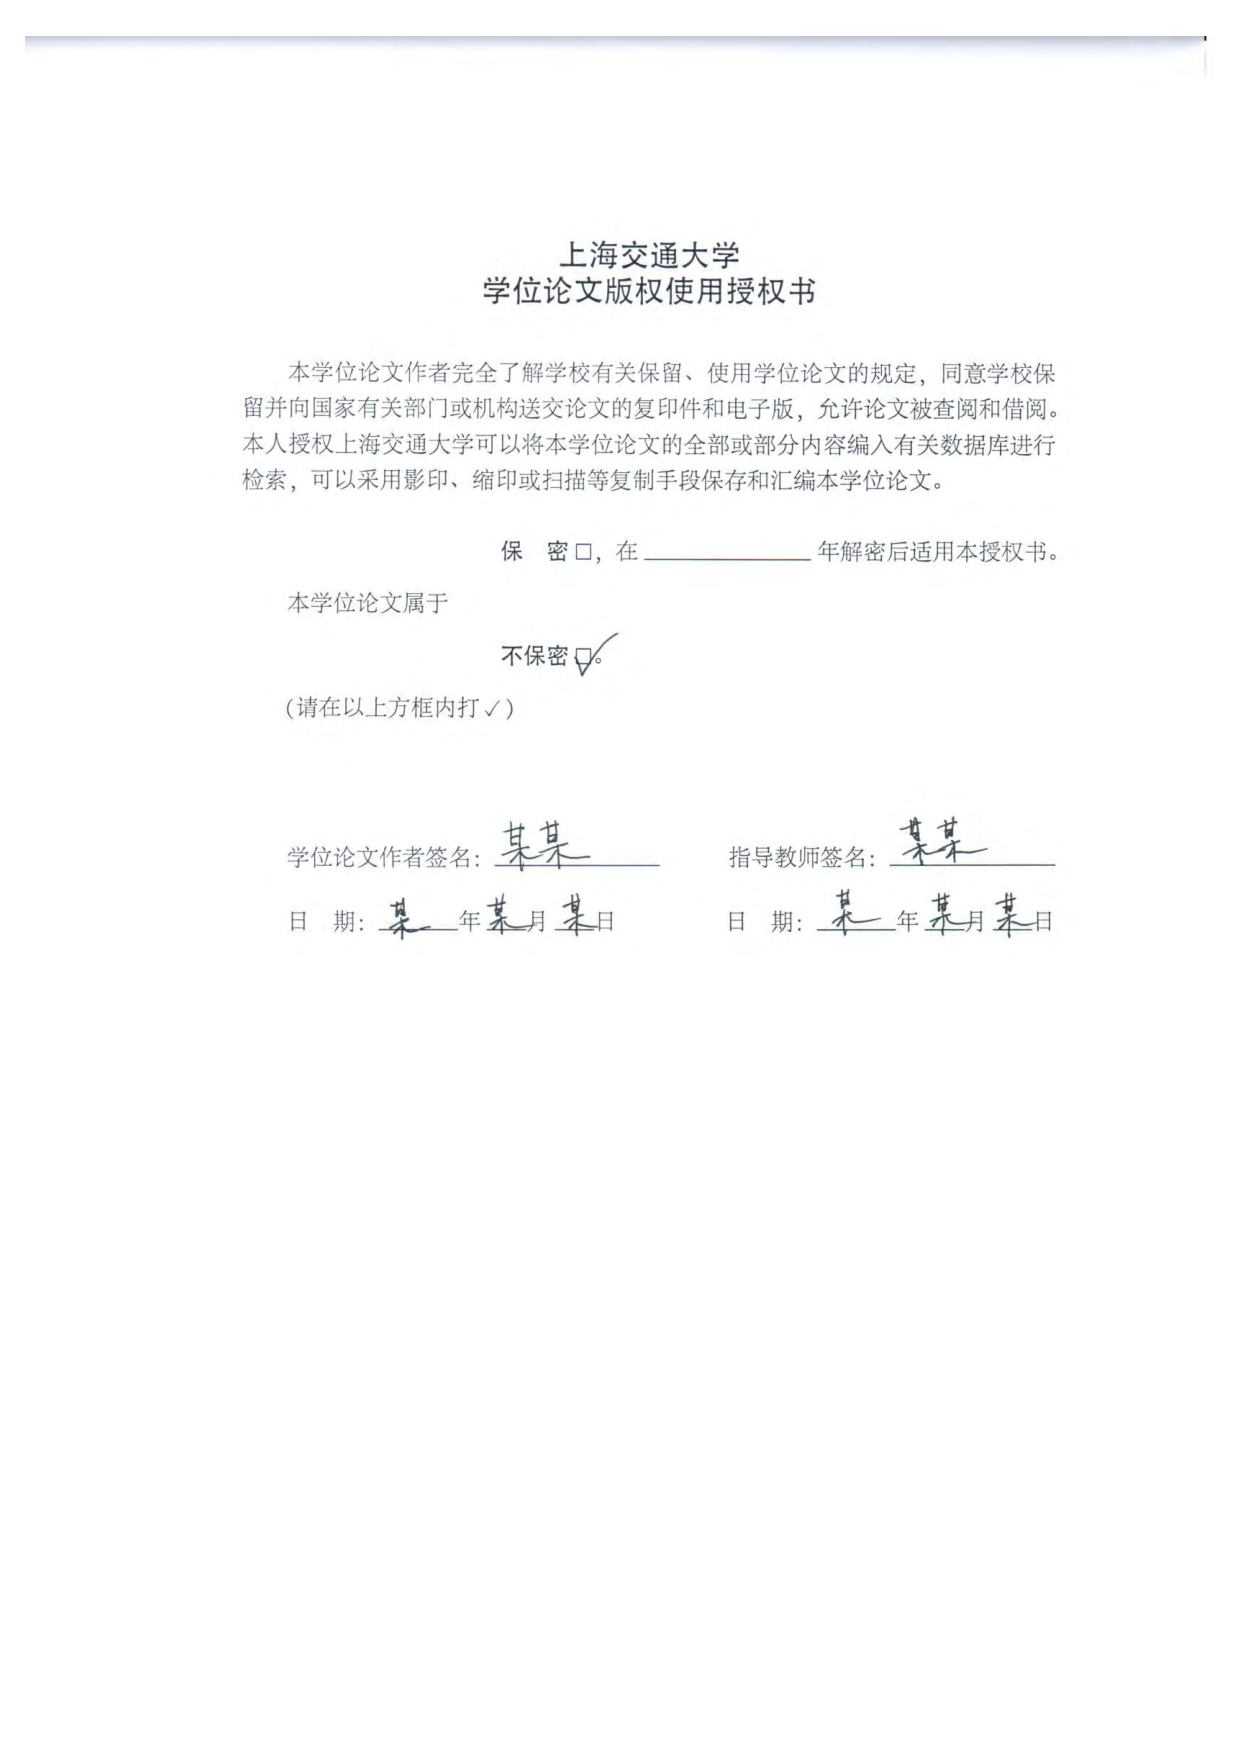
\includepdf{pdf/authorization.pdf}
  \cleardoublepage
\else
\ifsjtu@review\relax
% exclude the original claim and authorization
\else
  \makeDeclareOriginal
  \makeDeclareAuthorization
\fi
\fi
\makeatother

\frontmatter % 使用罗马数字对前言编号

% 摘要
%%# -*- coding: utf-8-unix -*-
% !TEX program = xelatex
% !TEX root = ../thesis.tex
% !TEX encoding = UTF-8 Unicode
%%==================================================
%% abstract.tex for SJTU Master Thesis
%%==================================================

\begin{abstract}

上海交通大学是我国历史最悠久的高等学府之一,是教育部直属、教育部与上海市共建的全国重点大学,是国家 “七五”、“八五”重点建设和“211工程”、“985工程”的首批建设高校。经过115年的不懈努力,上海交通大学已经成为一所“综合性、研究型、国际化”的国内一流、国际知名大学,并正在向世界一流大学稳步迈进。 

十九世纪末,甲午战败,民族危难。中国近代著名实业家、教育家盛宣怀和一批有识之士秉持“自强首在储才,储才必先兴学”的信念,于1896年在上海创办了交通大学的前身——南洋公学。建校伊始,学校即坚持“求实学,务实业”的宗旨,以培养“第一等人才”为教育目标,精勤进取,笃行不倦,在二十世纪二三十年代已成为国内著名的高等学府,被誉为“东方MIT”。抗战时期,广大师生历尽艰难,移转租界,内迁重庆,坚持办学,不少学生投笔从戎,浴血沙场。解放前夕,广大师生积极投身民主革命,学校被誉为“民主堡垒”。

新中国成立初期,为配合国家经济建设的需要,学校调整出相当一部分优势专业、师资设备,支持国内兄弟院校的发展。五十年代中期,学校又响应国家建设大西北的号召,根据国务院决定,部分迁往西安,分为交通大学上海部分和西安部分。1959年3月两部分同时被列为全国重点大学,7月经国务院批准分别独立建制,交通大学上海部分启用“上海交通大学”校名。历经西迁、两地办学、独立办学等变迁,为构建新中国的高等教育体系,促进社会主义建设做出了重要贡献。六七十年代,学校先后归属国防科工委和六机部领导,积极投身国防人才培养和国防科研,为“两弹一星”和国防现代化做出了巨大贡献。

改革开放以来,学校以“敢为天下先”的精神,大胆推进改革:率先组成教授代表团访问美国,率先实行校内管理体制改革,率先接受海外友人巨资捐赠等,有力地推动了学校的教学科研改革。1984年,邓小平同志亲切接见了学校领导和师生代表,对学校的各项改革给予了充分肯定。在国家和上海市的大力支持下,学校以“上水平、创一流”为目标,以学科建设为龙头,先后恢复和兴建了理科、管理学科、生命学科、法学和人文学科等。1999年,上海农学院并入;2005年,与上海第二医科大学强强合并。至此,学校完成了综合性大学的学科布局。近年来,通过国家“985工程”和“211工程”的建设,学校高层次人才日渐汇聚,科研实力快速提升,实现了向研究型大学的转变。与此同时,学校通过与美国密西根大学等世界一流大学的合作办学,实施国际化战略取得重要突破。1985年开始闵行校区建设,历经20多年,已基本建设成设施完善,环境优美的现代化大学校园,并已完成了办学重心向闵行校区的转移。学校现有徐汇、闵行、法华、七宝和重庆南路(卢湾)5个校区,总占地面积4840亩。通过一系列的改革和建设,学校的各项办学指标大幅度上升,实现了跨越式发展,整体实力显著增强,为建设世界一流大学奠定了坚实的基础。

交通大学始终把人才培养作为办学的根本任务。一百多年来,学校为国家和社会培养了20余万各类优秀人才,包括一批杰出的政治家、科学家、社会活动家、实业家、工程技术专家和医学专家,如江泽民、陆定一、丁关根、汪道涵、钱学森、吴文俊、徐光宪、张光斗、黄炎培、邵力子、李叔同、蔡锷、邹韬奋、陈敏章、王振义、陈竺等。在中国科学院、中国工程院院士中,有200余位交大校友;在国家23位“两弹一星”功臣中,有6位交大校友;在18位国家最高科学技术奖获得者中,有3位来自交大。交大创造了中国近现代发展史上的诸多“第一”:中国最早的内燃机、最早的电机、最早的中文打字机等;新中国第一艘万吨轮、第一艘核潜艇、第一艘气垫船、第一艘水翼艇、自主设计的第一代战斗机、第一枚运载火箭、第一颗人造卫星、第一例心脏二尖瓣分离术、第一例成功移植同种原位肝手术、第一例成功抢救大面积烧伤病人手术等,都凝聚着交大师生和校友的心血智慧。改革开放以来,一批年轻的校友已在世界各地、各行各业崭露头角。

截至2011年12月31日,学校共有24个学院/直属系(另有继续教育学院、技术学院和国际教育学院),19个直属单位,12家附属医院,全日制本科生16802人、研究生24495人(其中博士研究生5059人);有专任教师2979名,其中教授835名;中国科学院院士15名,中国工程院院士20名,中组部“千人计划”49名,“长江学者”95名,国家杰出青年基金获得者80名,国家重点基础研究发展计划(973计划)首席科学家24名,国家重大科学研究计划首席科学家9名,国家基金委创新研究群体6个,教育部创新团队17个。

学校现有本科专业68个,涵盖经济学、法学、文学、理学、工学、农学、医学、管理学和艺术等九个学科门类;拥有国家级教学及人才培养基地7个,国家级校外实践教育基地5个,国家级实验教学示范中心5个,上海市实验教学示范中心4个;有国家级教学团队8个,上海市教学团队15个;有国家级教学名师7人,上海市教学名师35人;有国家级精品课程46门,上海市精品课程117门;有国家级双语示范课程7门;2001、2005和2009年,作为第一完成单位,共获得国家级教学成果37项、上海市教学成果157项。

\end{abstract}

\begin{englishabstract}

An imperial edict issued in 1896 by Emperor Guangxu, established Nanyang Public School in Shanghai. The normal school, school of foreign studies, middle school and a high school were established. Sheng Xuanhuai, the person responsible for proposing the idea to the emperor, became the first president and is regarded as the founder of the university.

During the 1930s, the university gained a reputation of nurturing top engineers. After the foundation of People's Republic, some faculties were transferred to other universities. A significant amount of its faculty were sent in 1956, by the national government, to Xi'an to help build up Xi'an Jiao Tong University in western China. Afterwards, the school was officially renamed Shanghai Jiao Tong University.

Since the reform and opening up policy in China, SJTU has taken the lead in management reform of institutions for higher education, regaining its vigor and vitality with an unprecedented momentum of growth. SJTU includes five beautiful campuses, Xuhui, Minhang, Luwan Qibao, and Fahua, taking up an area of about 3,225,833 m2. A number of disciplines have been advancing towards the top echelon internationally, and a batch of burgeoning branches of learning have taken an important position domestically.

Today SJTU has 31 schools (departments), 63 undergraduate programs, 250 masters-degree programs, 203 Ph.D. programs, 28 post-doctorate programs, and 11 state key laboratories and national engineering research centers.

SJTU boasts a large number of famous scientists and professors, including 35 academics of the Academy of Sciences and Academy of Engineering, 95 accredited professors and chair professors of the "Cheung Kong Scholars Program" and more than 2,000 professors and associate professors.

Its total enrollment of students amounts to 35,929, of which 1,564 are international students. There are 16,802 undergraduates, and 17,563 masters and Ph.D. candidates. After more than a century of operation, Jiao Tong University has inherited the old tradition of "high starting points, solid foundation, strict requirements and extensive practice." Students from SJTU have won top prizes in various competitions, including ACM International Collegiate Programming Contest, International Mathematical Contest in Modeling and Electronics Design Contests. Famous alumni include Jiang Zemin, Lu Dingyi, Ding Guangen, Wang Daohan, Qian Xuesen, Wu Wenjun, Zou Taofen, Mao Yisheng, Cai Er, Huang Yanpei, Shao Lizi, Wang An and many more. More than 200 of the academics of the Chinese Academy of Sciences and Chinese Academy of Engineering are alumni of Jiao Tong University.

\end{englishabstract}



% 目录、插图目录、表格目录
\tableofcontents
\listoffigures
\addcontentsline{toc}{chapter}{\listfigurename}     % 将插图目录加入全文目录
\listoftables
\addcontentsline{toc}{chapter}{\listtablename}      % 将表格目录加入全文目录
\listofalgorithms
\addcontentsline{toc}{chapter}{\listalgorithmname}  % 将算法目录加入全文目录

%%# -*- coding: utf-8-unix -*-
% !TEX program = xelatex
% !TEX root = ../thesis.tex
% !TEX encoding = UTF-8 Unicode
\begin{nomenclaturename}
\label{chap:symb}

\begin{longtable}{rl}
$\epsilon$     & 介电常数 \\
 $\mu$ 		& 磁导率 \\
 $\epsilon$     & 介电常数 \\
 $\mu$ 		& 磁导率 \\
 $\epsilon$     & 介电常数 \\
 $\mu$ 		& 磁导率 \\
 $\epsilon$ 	& 介电常数 \\
 $\mu$ 		& 磁导率 \\
 $\epsilon$     & 介电常数 \\
 $\mu$ 		& 磁导率 \\
 $\epsilon$     & 介电常数 \\
 $\mu$ 		& 磁导率 \\
 $\epsilon$     & 介电常数 \\
 $\mu$ 		& 磁导率 \\
 $\epsilon$ 	& 介电常数 \\
 $\mu$ 		& 磁导率 \\
 $\epsilon$     & 介电常数 \\
 $\mu$ 		& 磁导率 \\
 $\epsilon$     & 介电常数 \\
 $\mu$ 		& 磁导率 \\
 $\epsilon$     & 介电常数 \\
 $\mu$ 		& 磁导率 \\
 $\epsilon$ 	& 介电常数 \\
 $\mu$ 		& 磁导率 \\
 $\epsilon$     & 介电常数 \\
 $\mu$ 		& 磁导率 \\
 $\epsilon$     & 介电常数 \\
 $\mu$ 		& 磁导率 \\
 $\epsilon$     & 介电常数 \\
 $\mu$ 		& 磁导率 \\
 $\epsilon$ 	& 介电常数 \\
 $\mu$ 		& 磁导率 \\
 $\epsilon$     & 介电常数 \\
 $\mu$ 		& 磁导率 \\
 $\epsilon$     & 介电常数 \\
 $\mu$ 		& 磁导率 \\
 $\epsilon$     & 介电常数 \\
 $\mu$ 		& 磁导率 \\
 $\epsilon$ 	& 介电常数 \\
 $\mu$ 		& 磁导率 \\
 $\epsilon$     & 介电常数 \\
 $\mu$ 		& 磁导率 \\
 $\epsilon$     & 介电常数 \\
 $\mu$ 		& 磁导率 \\
 $\epsilon$     & 介电常数 \\
 $\mu$ 		& 磁导率 \\
 $\epsilon$ 	& 介电常数 \\
 $\mu$ 		& 磁导率 \\
 $\epsilon$     & 介电常数 \\
 $\mu$ 		& 磁导率 \\
 $\epsilon$     & 介电常数 \\
 $\mu$ 		& 磁导率 \\
 $\epsilon$     & 介电常数 \\
 $\mu$ 		& 磁导率 \\
\end{longtable}

\end{nomenclaturename}
 % 主要符号、缩略词对照表

\mainmatter % 使用阿拉伯数字对正文编号

% 正文内容
%%# -*- coding: utf-8-unix -*-
% !TEX program = xelatex
% !TEX root = ../thesis.tex
% !TEX encoding = UTF-8 Unicode
%%==================================================
%% chapter01.tex for SJTU Master Thesis
%%==================================================

%\bibliographystyle{sjtu2}%[此处用于每章都生产参考文献]
\chapter{这是什么}
\label{chap:intro}

这是上海交通大学(非官方)学位论文 \LaTeX 模板,当前版本是 \version 。

最早的一版学位模板是一位热心的物理系同学制作的。
那份模板参考了自动化所学位论文模板,使用了CASthesis.cls文档类,中文字符处理则采用当时最为流行的 \CJKLaTeX 方案。
我根据交大研究生院对学位论文的要求
\footnote{\url{http://www.gs.sjtu.edu.cn/policy/fileShow.ahtml?id=130}}
,结合少量个人审美喜好,完成了一份基本可用的交大 \LaTeX 学位论文模板。
但是,搭建一个 \CJKLaTeX 环境并不简单,单单在Linux下配置环境和添加中文字体,就足够让新手打退堂鼓。
在William Wang的建议下,我开始着手把模板向 \XeTeX 引擎移植。
他完成了最初的移植,多亏了他出色的工作,后续的改善工作也得以顺利进行。

随着我对 \LaTeX 系统认知增加,我又断断续续做了一些完善模板的工作,在原有硕士学位论文模板的基础上完成了交大学士和博士学位论文模板。

现在,交大学位论文模板SJTUTHesis代码在github
\footnote{\url{https://github.com/sjtug/SJTUThesis}}
上维护。
你可以\href{https://github.com/sjtug/SJTUThesis/issues}{在github上开issue}
、或者在\href{https://bbs.sjtu.edu.cn/bbsdoc?board=TeX_LaTeX}{水源LaTeX版}发帖来反映遇到的问题。

\section{使用模板}

\subsection{准备工作}
\label{sec:requirements}

要使用这个模板撰写学位论文,需要在\emph{TeX系统}、\emph{TeX技能}上有所准备。

\begin{itemize}[noitemsep,topsep=0pt,parsep=0pt,partopsep=0pt]
	\item {\TeX}系统:所使用的{\TeX}系统要支持 \XeTeX 引擎,且带有ctex 2.x宏包,以2017年或更新版本的\emph{完整}TeXLive、MacTeX发行版为佳。
	\item TeX技能:尽管提供了对模板的必要说明,但这不是一份“ \LaTeX 入门文档”。在使用前请先通读其他入门文档。
	\item 针对Windows用户的额外需求:学位论文模本分别使用git和GNUMake进行版本控制和构建,建议从Cygwin\footnote{\url{http://cygwin.com}}安装这两个工具。
\end{itemize}

\subsection{模板选项}
\label{sec:thesisoption}

sjtuthesis提供了一些常用选项,在thesis.tex在导入sjtuthesis模板类时,可以组合使用。
这些选项包括:

\begin{itemize}[noitemsep,topsep=0pt,parsep=0pt,partopsep=0pt]
	\item 学位类型:bachelor(学位)、master(硕士)、doctor(博士),是必选项。
	\item 中文字体:fandol(Fandol 开源字体)、windows(Windows 系统下的中文字体)、mac(macOS 系统下的华文字体)、ubuntu(Ubuntu 系统下的文泉驿和文鼎字体)、adobe(Adobe 公司的中文字体)、founder(方正公司的中文字体),默认根据操作系统自动配置。
	\item 英文模版:使用english选项启用英文模版。
	\item 盲审选项:使用review选项后,论文作者、学号、导师姓名、致谢、发表论文和参与项目将被隐去。
\end{itemize}

\subsection{编译模板}
\label{sec:process}

模板默认使用GNUMake构建,GNUMake将调用latemk工具自动完成模板多轮编译:

\begin{lstlisting}[basicstyle=\small\ttfamily, caption={编译模板}, numbers=none]
make clean thesis.pdf
\end{lstlisting}

若需要生成包含“原创性声明扫描件”的学位论文文档,请将扫描件保存为statement.pdf,然后调用make生成submit.pdf。

\begin{lstlisting}[basicstyle=\small\ttfamily, caption={生成用于提交的学位论文}, numbers=none]
make clean submit.pdf
\end{lstlisting}

编译失败时,可以尝试手动逐次编译,定位故障。

\begin{lstlisting}[basicstyle=\small\ttfamily, caption={手动逐次编译}, numbers=none]
xelatex -no-pdf thesis
biber --debug thesis
xelatex thesis
xelatex thesis
\end{lstlisting}

\subsection{模板文件布局}
\label{sec:layout}

\begin{lstlisting}[basicstyle=\small\ttfamily,caption={模板文件布局},label=layout,float,numbers=none]
├── LICENSE
├── Makefile
├── README.md
├── bib
│   ├── chap1.bib
│   └── chap2.bib
├── bst
│   └── GBT7714-2005NLang.bst
├── figure
│   ├── chap2
│   │   ├── sjtulogo.eps
│   │   ├── sjtulogo.jpg
│   │   ├── sjtulogo.pdf
│   │   └── sjtulogo.png
│   └── sjtubanner.png
├── sjtuthesis.cfg
├── sjtuthesis.cls
├── statement.pdf
├── submit.pdf
├── tex
│   ├── abstract.tex
│   ├── ack.tex
│   ├── app_cjk.tex
│   ├── app_eq.tex
│   ├── app_log.tex
│   ├── chapter01.tex
│   ├── chapter02.tex
│   ├── chapter03.tex
│   ├── conclusion.tex
│   ├── id.tex
│   ├── patents.tex
│   ├── projects.tex
│   ├── pub.tex
│   └── symbol.tex
└── thesis.tex
\end{lstlisting}

本节介绍学位论文模板中木要文件和目录的功能。

\subsubsection{格式控制文件}
\label{sec:format}

格式控制文件控制着论文的表现形式,包括sjtuthesis.cfg和sjtuthesis.cls。
其中,“cls”控制论文主体格式,“cfg”为配置文件。

\subsubsection{主控文件thesis.tex}
\label{sec:thesistex}

主控文件thesis.tex的作用就是将你分散在多个文件中的内容“整合”成一篇完整的论文。
使用这个模板撰写学位论文时,你的学位论文内容和素材会被“拆散”到各个文件中:
譬如各章正文、各个附录、各章参考文献等等。
在thesis.tex中通过“include”命令将论文的各个部分包含进来,从而形成一篇结构完成的论文。
对模板定制时引入的宏包,建议放在导言区。

\subsubsection{各章源文件tex}
\label{sec:thesisbody}

这一部分是论文的主体,是以“章”为单位划分的,包括:

\begin{itemize}[noitemsep,topsep=0pt,parsep=0pt,partopsep=0pt]
	\item 中英文摘要(abstract.tex)。前言(frontmatter)的其他部分,中英文封面、原创性声明、授权信息在sjtuthesis.cls中定义,不单独分离为tex文件。
不单独弄成文件。
	\item 正文(mainmatter)——学位论文正文的各章内容,源文件是chapter\emph{xxx}.tex。
	\item 附录(app\emph{xx}.tex)、致谢(ack.tex)、攻读学位论文期间发表的学术论文目录(pub.tex)、个人简历(resume.tex)组成正文后的部分(backmatter)。
参考文献列表由bibtex插入,不作为一个单独的文件。
\end{itemize}

\subsubsection{图片文件夹figure}
\label{sec:fig}

figure文件夹放置了需要插入文档中的图片文件(支持PNG/JPG/PDF/EPS格式的图片),可以在按照章节划分子目录。
模板文件中使用\verb|\graphicspath|命令定义了图片存储的顶层目录,在插入图片时,顶层目录名“figure”可省略。

\subsubsection{参考文献数据库bib}
\label{sec:bib}

目前参考文件数据库目录只存放一个参考文件数据库thesis.bib。
关于参考文献引用,可参考第\ref{chap:example}章中的例子。


%# -*- coding: utf-8-unix -*-
% !TEX program = xelatex
% !TEX root = ../thesis.tex
% !TEX encoding = UTF-8 Unicode
%%==================================================
%% chapter01.tex for SJTU Master Thesis
%%第一章
%%==================================================
\chapter{绪论}
\section{课题背景及研究意义}
\subsection{课题研究背景}
人工智能(Artificial Intelligence,AI)是研究,开发用于模拟延伸和扩展人的认知,识别,分析和决策的多种功能的一门新兴科学技术,同时涵盖了统计学,计算机科学,脑神经科学和社会科学等学科。人工智能的应用领域包括机器人,语音识别,图像识别,自然语言处理和专家系统等等。从人工智能被首次提出到现在还不到一个世纪的时间里,由于科技发展水平的阻力已经经历了几次大起大落:1956年在达特茅斯会上将不同研究领域的学者组织在一起,首次提出了人工智能的概念,标志着人工智能成为一个独立的研究领域。美国国防部高级研究计划局拨款220万美元给MIT用于人工智能研究工作带来了AI的第一次高潮时期,在1970年前后,由于数据量不够加上算法实现能力不足,和基础研究理论薄弱,导致人工智能在商用和军用中失败,迎来了人工智能的第一次寒冬,80年代专家系统的诞生迎来了人工智能的第二个春天,知识库系统和知识工程都得到了普及,紧接着日本推进了第五代计算机项目,各国之间相继开展计算机科技竞赛。随着专家系统的不断发展,数据处理的复杂度快速提升,基于知识库和推理机的专家系统逐渐暴露出缺点,扩展维护工作开展困难,鲁棒性薄弱的缺点导致人工智能再次陷入低谷,随着神经网络的普及,算力的增长,在90 年代,国际象棋冠军卡斯帕罗夫与"深蓝" 计算机决战,"深蓝"获胜,公众再次把注意力放在了人工智能,在2016年,谷歌的AlphaGo赢了韩国棋手李世石,再度引发人工智能热潮。2018年腾讯人工智能实验室推出的“绝艺”在腾讯世界人工智能围棋大赛决赛中以7:0的比分战胜星战围棋\cite{人工智能产业形势分析课题组20182018},这些都代表了特定时期人工智能发展的技术水平。如图\ref{fig:人工智能发展历史图况}所示。

\begin{figure}[htb]
	\centering
	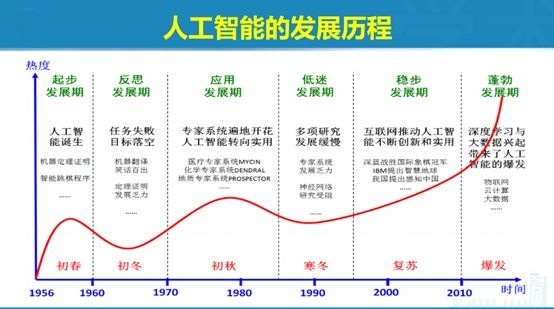
\includegraphics[width=15cm]{example/AI_history.jpg}
	\bicaption[这里将出现在插图索引]
	{人工智能发展历史图况.}
	{The history of Artificial Intelligence.}
	\label{fig:人工智能发展历史图况}
\end{figure}

人工智能的实现算法在现代被称为机器学习,根据机器学习的应用数据和模型任务,可以分成监督学习,无监督学习和强化学习。本文研究的深度强化学习是在强化学习的框架下引入了深度学习作为函数拟合的工具,下面分别介绍传统的强化学习和深度学习概念。

深度学习是机器学习的重要组成部分,深度学习是利用深层的神经网络进行函数的拟合工作用来建立更加复杂的模型,从而对数据有更深刻全面的理解。深度学习网络把原始数据通过简单的非线性函数进行映射,转换为高层次抽象的表达,通过加大神经网络的深度进行多次非线性映射堆叠,可以表示出非常复杂的模型。通过在学习过程中引入紧缩性和鲁棒性的约束,网络后端的特征输出部分不仅可以强化对输入数据的区分和预测能力,同时可以避免外界噪声和其他不相关因素的干扰,因此在浅层网络无法全面客观表示数据特征,学习数据分布的时候可以采用深度学习网络进行统一的特征学习框架的搭建。深度学习各层的输入特征不是根据具体任务人为处理的,而是利用一种通用的映射和优化的过程从原始数据中学习得到。特征提取工作和分类预测任务被深度学习框架进行统一整合,避免了繁琐的人类手工设计提取特征的过程,实现了端到端的自动学习。准确的说深度学习首先利用无监督学习对每一层的网络节点进行预训练学习模型,并将当前层的输出数据作为输入数据传入给下一层,最后一层采用监督学习方式,根据网络的最后一层输出结果进行前向传播进行网络参数的整体微调优化。经过若干次的参数迭代可以得到相对稳定的网络结构。深度学习的发展过程如图\ref{fig:test}。
\begin{figure}[htpb]
	\centering
	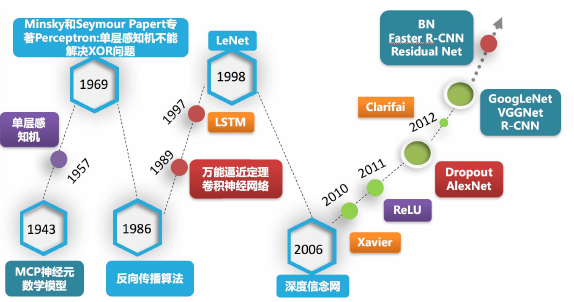
\includegraphics[width=15cm]{example/Deep_Learning_history.png}
	\bicaption[这里将出现在插图索引]
	{人工智能发展历史图况.}
	{The history of Artificial Intelligence.}
	\label{fig:test}
\end{figure}

伴随着AlphaGo的诞生,强化学习(Reinforcement Learning)作为其核心算法逐渐成为机器学习研究的另一大热点。从某种意义上讲,强化学习是人工智能的未来。有学者认为,智能系统必须能够在不接受持续监督的情况下自主学习,而强化学习正是其中的最佳代表。一个AI必须能够自己判断对错,只有这样才能扩展到大量的知识和一般技能。学习一个好的,而非新的表征对于解决大多数现实世界中的问题来说具有至关重要的作用这些表征通常不需要被显式地进行学习,这种学习可以通过内部奖励机制来进行引导,强化学习就是这样一种学习方式。机器学习是个跨学科的研究领域,而强化学习则是其中跨学科性质非常显著的一个分支。强化学习理论的发展受到生理学、神经科学和最优控制等领域的启发,现在依旧在很多相关领域被研究。在控制理论、机器人学、运筹学、经济学等领域内部,依旧有很多的学者投身RL的研究,类似的概念或算法往往在不同的领域被重新发明,起了不同的名字。

追随强化学习的发展历史,从1956年Bellman提出动态规划方法,到1977年提出的自适应动态规划算法以及1988年的时间差分算法,1922年Q-learning算法首次被提出,Q-learning也是目前应用最广的算法之一。后来又衍生出很多改进的强化学习算法,包括Saras算法,置信上限树算法,确定性策略梯度算法,等等。图\ref{fig:2}详细介绍了强化学习的发展历史。

\begin{figure}[htpb]
	\centering
	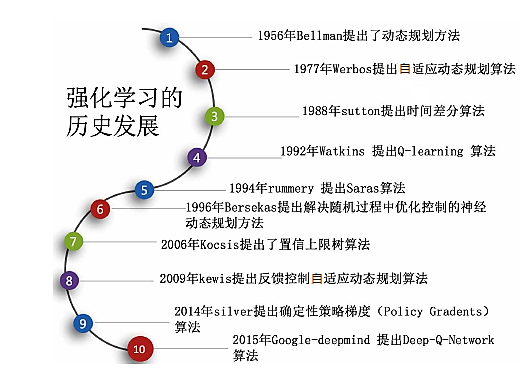
\includegraphics[width=15cm]{example/Reinforment_learning.png}
	\bicaption[这里将出现在插图索引]
	{强化学习发展历史}
	{The history of Artificial Intelligence.}
	\label{fig:2}
\end{figure}

强化学习被广泛应用在仿真模拟\cite{傅启明2014一种基于线性函数逼近的离策略}、工业制造\cite{高阳2007平均奖赏强化学习算法研究}、优化与调度\cite{魏英姿2005一种基于强化学习的作业车间动态调度方法},机器人控制\cite{Ipek2008Self}、游戏博弈\cite{Tesauro1944TD}等领域。

强化学习的核心思想就是以最大化累积奖励为目标,获取完成目标的最优决策方案,因此相比于其他机器学习算法,强化学习更加注重学习解决问题的策略。例如,微软利用强化学习为MSN上的新闻故事选标题,点击该标题的访问者越多,得到的奖励越多,这意味着一个良好的强化学习系统能够做到对明确的优化目标进行奖励最大化。Alphago围棋,也是强化学习的又一个重要的应用场景,在这里最核心的就是如何建立建立情景\raisebox{0.3mm}{----}动作映射(map situations to actions)。智能体并没有明确告知当前最优的动作选择,而是希望通过不断的尝试进行若干个相互关联的动作之后得到最大的总奖励和。当前的行动不仅会影响到即时收益和当前的状态空间的转移同样也会影响所有后续的奖励之和。因此,试错和延迟收益是强化学习两个重要特征。
\subsection{课题研究意义}
早期的强化学习需要人为干预特征的提取,然而人类的认知并不一定是全面完备的,人工提取特征进行标注同时需要消耗大量的资源。受深度学习提取特征的启发,通过深度学习网络代替手工设计的功能或领域启发式算法进行前期的特征提取工作,智能体直接从原始输入构建和获取自己的知识库,增强了强化学习的特征学习能力。这种利用深度学习工具进行特征构建和函数拟合的强化学习算法称为深度强化学习。
深度强化学习结合了深度学习感知能力强和传统强化学习优秀的决策能力的优点,通过端对端的学习方式实现了组合策略的能力,做到了对原始数据从输入到输出的直接控制。其算法的整体框架如图\ref{fig:DRL}所示。
\begin{figure}[h]
	\centering
	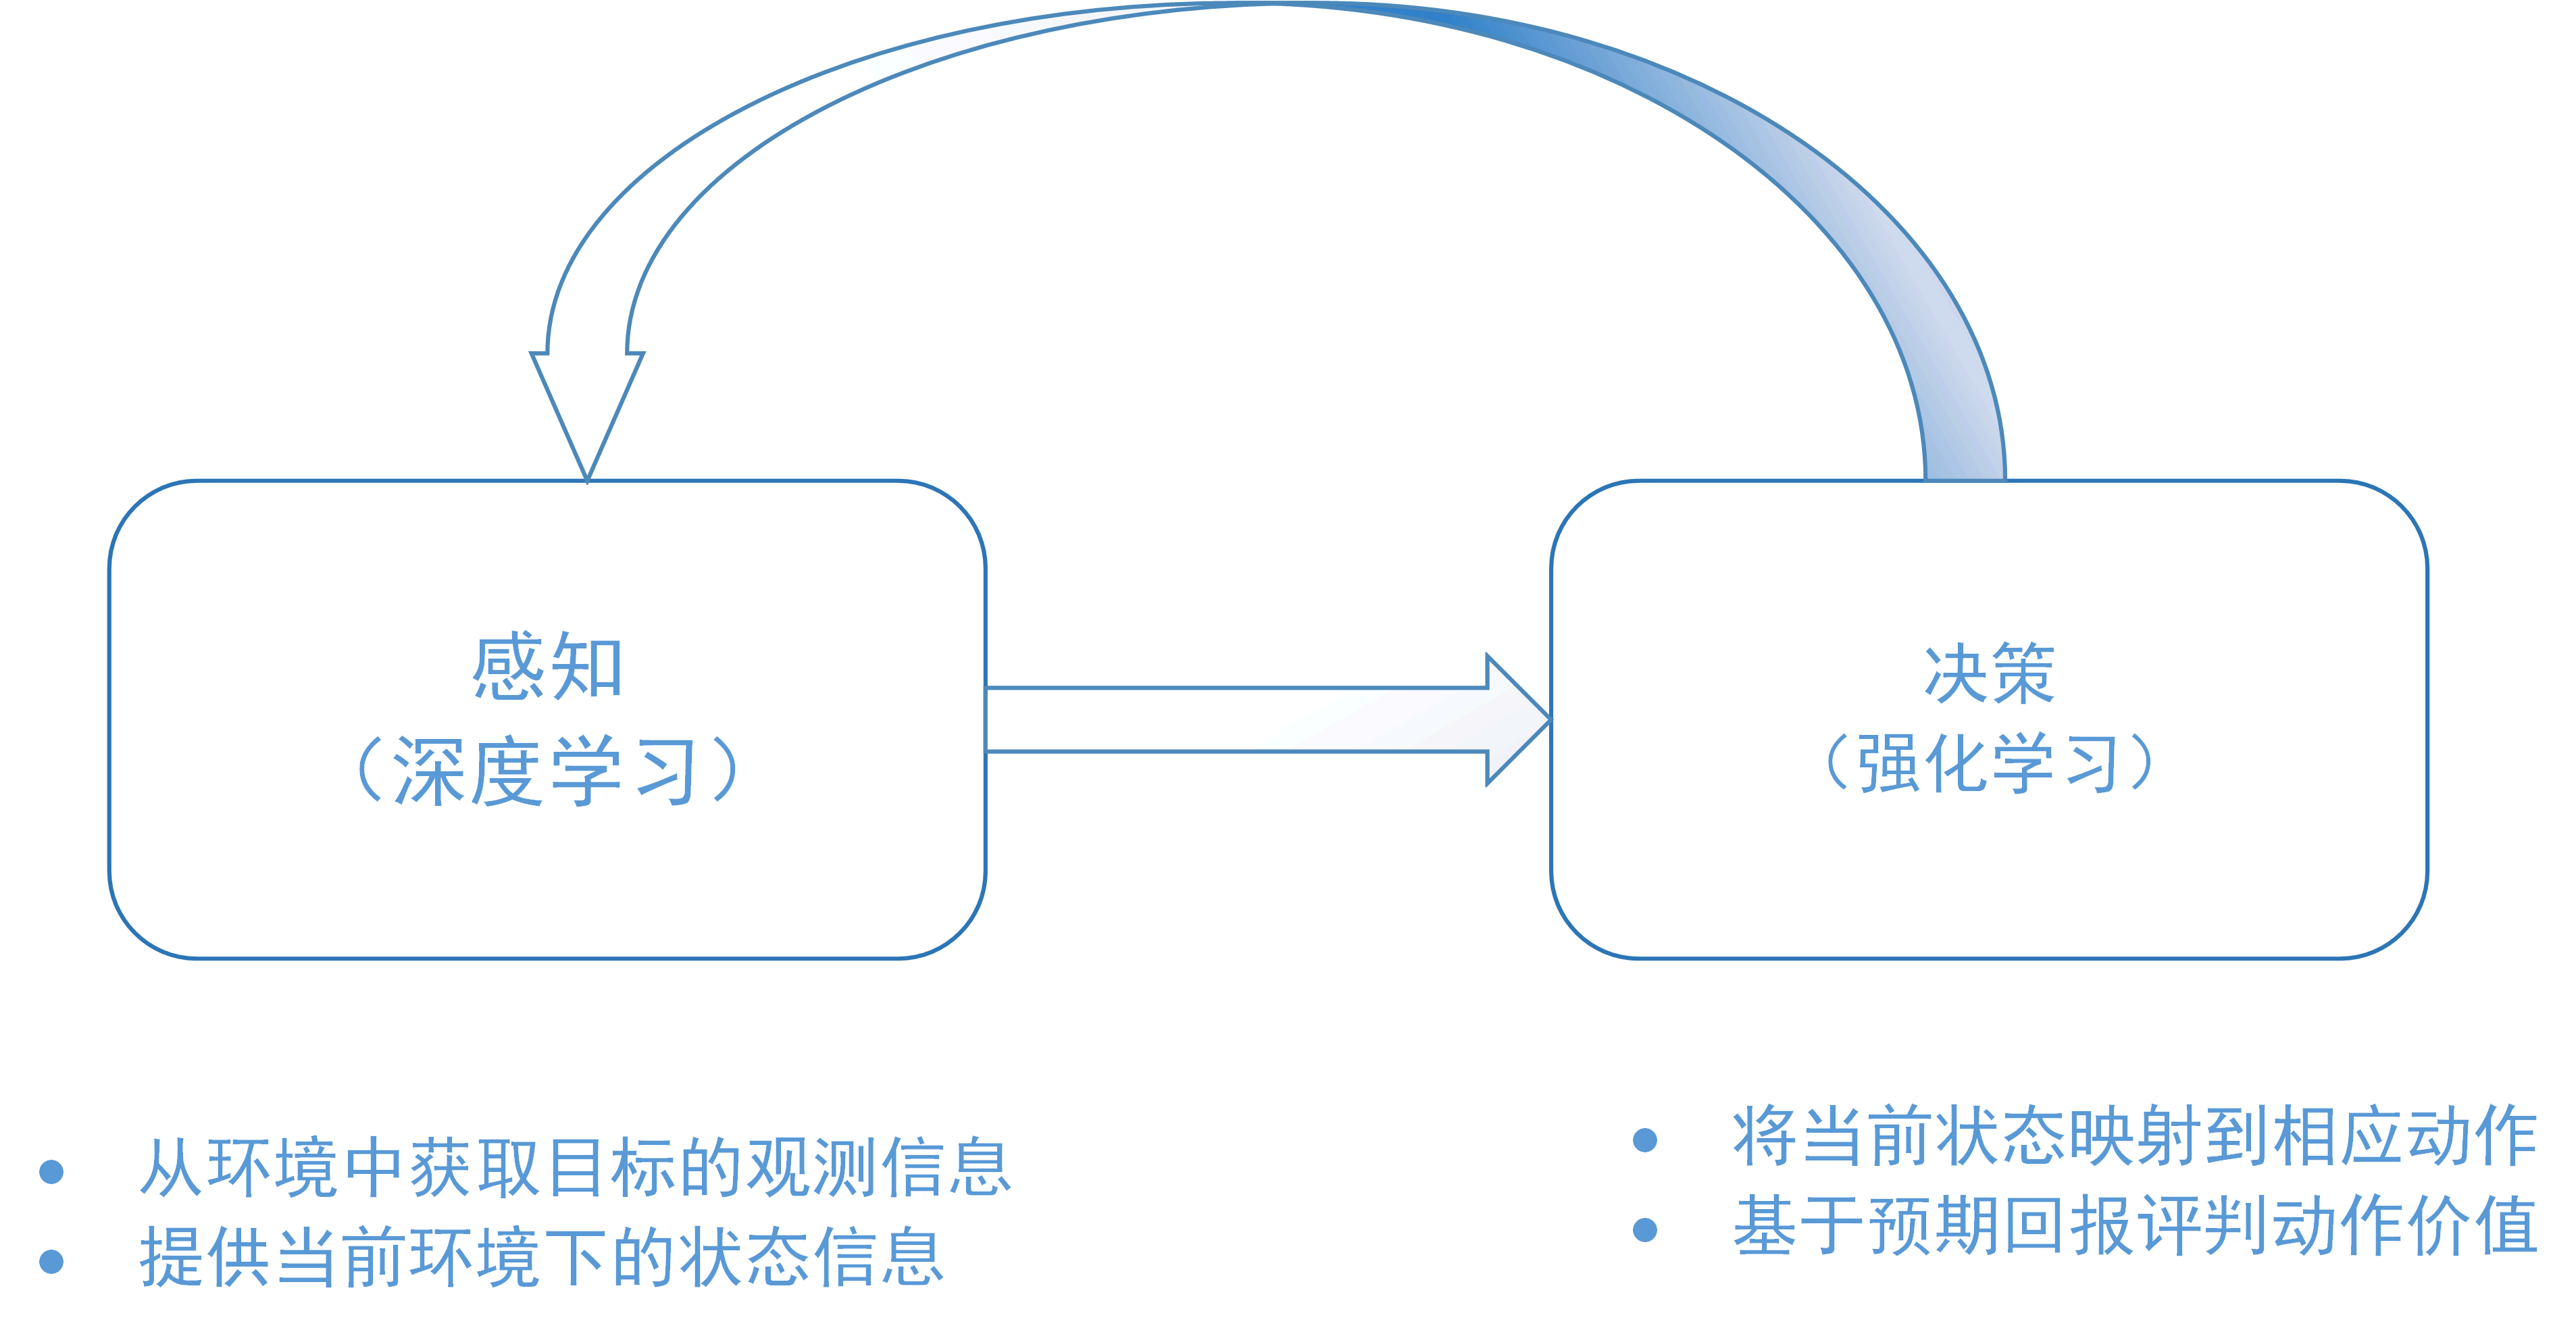
\includegraphics[width=\hsize]{example/DRL.png}
	\bicaption[这里将出现在插图索引]
	{深度强化学习框架}
	{The fremework of deep reinforcement learning}
	\label{DRL}
\end{figure}

近年来深度强化学习在以惊人的速度发展,各个团队相继在探索强化学习在不同领域的新方法和新应用。其进步的速度是有目共睹的,在不到两年的时间里,深度强化学习衍生了很多新算法,如:深度Q网络(Deep Q Network,DQN)\cite{Roderick2017Implementing}, AlphaGo\cite{Silver2016Mastering},以及可微分神经计算机\cite{Graves2016Hybrid},我们也见证了深度强化学习在很多应用上的进展,注意力和机制也都得到了很大的关注。在应用上,决斗网络(dueling network)架构\cite{Wang2015Dueling},ACL上的口语对话系统\cite{Su2016On},EMNLP上的信息提取\cite{Narasimhan2016Improving},以及 NIPS上的价值迭代网络(value iteration networks)\cite{Tamar2017Value}。激动人心的成就比比皆是:异步方法\cite{Mnih2016Asynchronous},用于机器翻译的双学习(dual learning)\cite{Xia2016Dual},生成对抗式模仿学习\cite{Ho2016Generative},无监督强化和辅助学习\cite{Jaderberg2016Reinforcement},神经架构设计\cite{Pham2018Efficient}等等。新的学习机制也在出现,例如把强化学习和无监督,半监督,迁移学习结合提升学习的质量和速度。新的强化学习算法还在不断涌现,学习模型会带来稳定性,收敛性,数据效率,可扩展性,速度,简洁性,可解释性,稳健性和安全性的问题,奖励反馈机制的建立也是很重要的一环,奖励可能来自认知科学领域,涉及物理学,因果模型,组合性学习等各个领域的知识。。强化学习作为一种更为通用的学习和决策范式,将会给深度学习、机器学习和广义上的人工智能带来深远的影响。

\section{深度强化学习国内外研究现状}
在高级人工智能领域,感知和决策都是衡量智能的重要指标。尽管强化学习在理论和算法层面已经取得了一系列的成就,然而通过直接感知高维数据的输入(如图像,语音等)去控制智能体,对强化学习来说仍是长期的任务和挑战。传统的强化学习算法大部分的成功应用方案依赖于人工特征的提取,学习结果的好坏严重依赖于特征选取的质量。深度学习具有较强的特征提取能力但是不具备决策能力,强化学习具有很强的决策能力,对感知问题束手无策,因此,将两者结合起来,优势互补,为复杂系统的感知与决策问题提供了有效的解决思路。

\subsection{深度强化学习国外研究成果}
深度强化学习研究的初期思路就说利用神经网络完成数据的降维任务,将较高维度的特征经过神经网络变换到较低维度,降低强化学习处理的难度。典型的应用包括利用千层神经网络提取视觉信号的输入,控制机器人推箱子\cite{Shibata2003Acquisition},将强化学习和深层自动编码机结合,利用“视觉动作学习”完善智能体的感知能力\cite{Lange2010Deep},将深度置信网络代替传统的值函数逼近器,用于车牌字符分割识别\cite{Abtahi2015A},深度拟合Q学习\cite{Lange2012Autonomousd}利用视觉输入信号结合深度强化学习框架用于车辆控制的问题,该算法的输入数据为跑道和车辆图像,通过深度学习网络提取特征利用Q学习最后输出合适的控制策略。同时期实现视频赛车自动驾驶策略规划的还有利用神经演化方法(neural evolution, NE)和强化学习进行结合\cite{Kumar2014Understanding}。

受上述前期工作的启发,卷积神经网络在图像处理领域的优秀表现使很多学者开始研究将卷积神经网络和强化学习算法进行结合处理图像数据的感知决策任务。深度Q网络(deep Q network, DQN)\cite{Mnih2013Playing}在2013年被深智团队首次提出,该算法的思想是将CNN网络和Q学习进行结合,利用经验回放技术优化网络。DQN网络是深度强化学习领域的突破,其输入数据是原始时间顺序上连续4帧的游戏画面,经过多层卷积神经网络和全连接网络,输出最后的状态动作Q函数,首次实现了端到端的学习控制。DQN网络的出现引发了深度强化学习的热潮,众多学者提出了很多改进方案,Schaul提出了带优先级经验回放的深度Q网络\cite{Schaul2015Prioritized},通过对经验进行先后顺序排序,增加相对重要历史数据的回放比例来提高学习效果,弥补了原来DQN网络经验回访技术没有考虑历史数据重要程度的缺点。为了改进Q网络训练过程缓慢的问题,Nair等提出了深度Q网络的大规模分布式架构Gorila\cite{Goeringer2013Massively},该方法极大的提高了深度Q网络的学习速率。Guo等首次将蒙特卡洛搜索树和原始深度Q网络结合\cite{Guo2014Deep},用于实时处理Atari游戏,效果好于原始深度Q网络。双重深度Q网络(double-DQN)\cite{DQN}将两个Q学习网络运用到深度Q网络中,得到更加稳定的学习策略,从而解决了原始Q网络中对由于固有估计误差造成的过高估计动作值函数的的问题。受优势学习(advantage learning)的启发,Wang等提出了一种适用于免模型学习(model free) 的竞争架构 (dueling architecture),实验结果表明,利用竞争架构的深度Q网络可以得到相对更加稳定的评估策略。解决探索和策略的问题一直是深度强化学习长期关注的核心,高效的探索策略用于解决复杂环境中的深度强化学习问题具有深远意义。Osband等首次提出一种引导式(boot-strapped)深度Q网络\cite{Osband2016Deep},引入了随机值函数提升了探索的速率和效率。为了加快强化学习的训练速率,Mnih等改进了异步深度强化学习方法\cite{Mnih2016Asynchronous}。
\subsection{深度强化学习国内研究成果}
中国的技术公司并不示弱,其实,他们做得更加激进,用深度强化学习做直接跟钱挂钩的业务落地。阿里、腾讯、百度、滴滴和天壤等国内团队将深度强化学习应用到搜索、推荐、营销、派单和路径规划等实际问题的决策任务中。并且有公司宣称自己使用了深度强化学习在无人驾驶产品中。
2018年阿里发行了第一本人工智能强化学习电子书\raisebox{0.3mm}{----}《从虚拟世界走进现实应用——强化学习在阿里的技术演进与业务创新》, 平台作为信息的载体,需要在与消费者的互动过程中,根据对消费者(环境)的理解,及时调整 提供信息(商品、客服机器的回答、路径选择等)的策略,从最化过程累 积收益(消费者在平台上的使体验)。基于监督学习式的信息提供段,缺少有效的探索能,系统倾向于给消费者推送曾经发过为的信息单元(商品、店铺或问题答案)。强化学习作为种有效的基于户与系统交互过程建模和最化过程累积收益的学习法,在某些具体的业务场景中进了很好的实践并得到大规模应。书中结合搜索场景,推荐场景,智能客服,广告系统等不同业务场景进行了详细的介绍。

从2016年起,腾讯AI Lab开始研发围棋人工智能程序,于2017年分别在“AI龙星战”和“UEC杯”等世界计算机围棋大赛上斩获冠军,2018年加强版的围棋智能程序“绝艺”问世,首次在让子棋中战胜顶级职业棋手柯洁九段和连笑九段。让子棋是人类通过人工智能不断探索围棋边界的典型范例。

百度也相继提出把强化学习应用在信息流质量的提升中,利用强化学习识别移除标题党,并在凤巢广告系统里部署了强化学习系统,充分利用了强化学习不需要数据标注,可以有效利用更多数据信息,能实现在线学习等优点。同时强化学习的部署也是对工程能力的挑战。在强化学习模型中,广告的优化行为是通过广告投放系统的所带来的奖励(点击率,转化率),观察广告竞价状态实现的。

深度强化学习通过不断的进步和发展, 在理论与应用层面取得了长足的进步. 表格\ref{tab:1}总结了深度强化学习发展历程中的重要事件。
\begin{table}[!hpb]
	\centering
	\bicaption[指向一个表格的表目录索引]
	{深度强化学习研究历程}
	{Timeline of deep reinforcement learning research events}
	\label{tab:1}
	\begin{tabular}{ll}
		年份 & 事件 \\ \midrule
		2013 & Mnih 等提出了深度强化学习的开创性工作DQN在视频游戏领域取得突破 \\
		2014& Guo 等提出DQN与MCTS结合的算法 \\
		2015 &Van 等提出了双重深度Q网络(double-DQN) \\
		2015&Hausknecht等结合LSTM提出了深度递归Q网络(DRQN)\\
		2015&Sorokin等结合注意力网络提出了深度注意力递归Q网络(DARQN)\\
		2016&深智团队在《Nature》上面发表了基于DRL的计算机围棋程序-Alphago\\
		2017&深智团队改进AlphaZero问世\\
		2018&腾讯AI LAb的“绝艺”斩获冠军\\
		 \bottomrule
	\end{tabular}
\end{table}
\subsection{现有研究不足和展望}
尽管随着深度强化学习的不断发展,越来越多的实际问题得到了有效的解决,深度强化学习在理论方面和应用方面仍然存在很多不足之处,如何有效解决这些缺点并拓展强化学习的应用场景将成为以后研究的重点方向。
不足包括:
\begin{enumerate}
	\item 当强化学习智能体的动作具体到生成数据时变成了生成式对抗网络(Generative Adversarial Networks,GAN),现有的生成式对抗网络模型大多数应用于图像视频数据的生成任务上,应用于非图像类数据的场景比较少,同时存在模式崩溃,生成样本数据分布覆盖不足的缺点。
	\item 深度强化学习的另一个主要应用于Atari视频游戏的自主决策,在这里的奖励是通过不断和游戏环境进行交互得到的。在其他应用场景奖励函数的选择和设计显得尤为重要。深度强化学习模型的泛化能力较弱,对于某些场景下表现效果好的模型不一定适用于其他场景。所以模型效果也直接依赖于环境的搭建。
	\item 目前强化学习解决实际问题中最成功的应用是与蒙特卡罗树搜索结合的方法进行一对一智能体两人零和完全信息博弈。多智能体博弈,包括零和,非零和,完全信息,不完全信息博弈的问题都需要进一步研究和扩展。机器学习算法的前提是数据在相同的特征空间具有相同的数据分布,但是现实环境的模型是比较复杂的,这种强制假设限制了深度强化学习的应用范围。可以考虑结合其他模型突破同数据分布的假设。
	\item 深度强化学习奖励反馈机制的建立是又一大难题,在部分应用场景反馈可以是确定性函数,但是大部分的应用场景反馈来自和环境的交互,所以需要把深度强化学习知识和其他学科进行结合,包括心理学,数据科学,计算机科学,神经网络感知科学,等等。
	\item 虽然深度强化学习有广阔的应用前景有待挖掘,但是很多应用者对于其理论层面的研究还不够深入,目前为止深度强化学习相关的文章并没有给出其学习过程收敛性的证明,只能通过是实验结果观察模型的学习效果。对模型的准确认知对于模型的完善和应用是非常关键的。从长远发展来看,理论基础的夯实会利于深度强化学习的良性发展。
\end{enumerate}
\section{主要内容与章节安排}
\subsection{本文的主要工作和创新点}
针对强化学习的应用现状和现有数据集和任务,本文的创新点如下:
\begin{enumerate}
	\item 具体化强化学习任务,利用GAN生成式对抗网络对数据集进行扩充和预测,并在现有WGAN网络的基础上引入监督信息,完善学习数据分布信息。
	\item 利用self-paly方式不依赖于人类专家数据进行智能体博弈仿真数据生成,引入自适应学习率和温度探索参数,并以五子棋为例进行实验效果分析。
	\item 由一对一智能体对抗拓展到多智能体之间的对抗和合作,设计实验场景并进行实验分析。
\end{enumerate}
\subsection{本文的内容安排}
本文主要研究深度强化学习原理及应用。通过对不同强化学习模型的研究和对比,本文实现了基于GAN生成式对抗网络的数据扩充和预测,利用AC模型的单智能体一对一仿真,和利用DDPG模型的多智能体对抗仿真。
具体的研究内容和章节安排如下:

第一章 绪论。说明了本课题的背景及研究意义,指出存在的技术难点,介绍了目前国内外深度强化学习的研究概况。

第二章主要介绍了传统的强化学习的种类和基本原理,以及结合深度学习模型改进之后的强化学习模型的各种变体原理及相关应用。并结合Alphago以及Alphazero的实现过程剖析背后的主要技术。

第三章针对小样本本缺失数据扩充的具体问题,利用不同的数据集,包括电子设备参数数据的扩充以及不同股票收盘指数数据,经过前期数据处理后进行数据的扩充,由于GAN网络应用场景主要是图像数据,在本章节提出针对数值类数据的改进的引入监督信息的GAN生成式对抗网络对数据进行扩充和预测,利用实验结果分析模型的收敛性以及数据扩充效果。

第四章针对智能体一对一对抗策略的问题,提出了类比Alphazero原理的的无先验数据进行训练的Actor-Critic强化学习模型,该模型结合了深度学习强大的拟合能力,利用深度学习网络拟合动作概率函数以及估值网络进行策略选择,用self-paly的形式进行两个智能体相互博弈进行数据的生成和扩充,同时利用蒙特卡洛搜索树进行结果的预测,实验结果给出了最后智能体作战的策略以及训练的损失函数曲线分析,证明了模型的收敛性。

第五章针对多个智能体分成两方作战的问题,利用MADDPG模型。为每个智能体建立单独的Actor网络和Critic网络,实现了集中训练和分布执行的训练方式,每个智能体都能感知其他智能体的动作以及全局的状态,每个Agent的Critic输入除自身的state-action信息外,还可以有额外的信息,比如其他Agent的动作。实验的最后分析了算法的可行性以及对智能体作战结果的剖析。

第六章综合了所提出的几种模型,把不同算法集成到一个可执行软件中,通过GUI界面实现各章工作成果的直观展示。

第七章总结全文研究内容,针对本文目前研究的不足对今后的工作提出展望。

%# -*- coding: utf-8-unix -*-
% !TEX program = xelatex
% !TEX root = ../thesis.tex
% !TEX encoding = UTF-8 Unicode
%%==================================================
%% chapter01.tex for SJTU Master Thesis
%%第二章
%%==================================================
\chapter{深度强化学习介绍}
深度强化学习结合了深度学习强大的感知能力和强化学习优秀的决策能力,本章将以传统强化学习为切入点,介绍强化学习相关理论知识并深入介绍几种典型的深度强化学习算法,作为后续章节的铺垫。

\section{强化学习简介}
强化学习是一个由行为心理学引导出来的面向目标的机器学习领域。其研究的目标就是在和环境不断交互的过程中,经过一系列的决策过程达到累计奖励值最大化的过程。强化学习和监督学习的区别主要有以下两点:不同于监督学习根据历史经验感知周围的环境,强化学习没有明确的标签信息,是通过不断进行尝试和环境进行交互根据结果进一步优化决策信息。可以说强化学习是一种具有标签延迟的监督学习。监督学习的前提是数据独立同分布的,而强化学习本身没有这个约束,其模型的前提是数据基于高度序列化,智能体当前的动作会影响到下一时刻。

\subsection{强化学习基本概念}

强化学习的研究离不开以下几个组成成分:

\begin{enumerate}
	\item 智能体(Agent):智能体被定义为有智慧的决策体,是策略的承载体。
	\item 动作(Action,A): $ S=\{a_{0},a_{1},a_{2},\dots,a_{n}\} $作为智能体采取动作的集合,智能体从动作列表集合里选取合适的动作,进行与周围环境的交互过程。在这里动作可以是离散的也可以是连续的。
	\item 环境(Environment):环境包含了智能体当前的状态和行为动作的输入。同时根据智能体选择动作的变化输出下一个状态和奖励反馈信息。通常环境蕴含了一定的物理模型规律或社会规则。
	\item 状态(State,S): $ S=\{s_{0},s_{1},s_{2},\dots,s_{n}\} $状态反应显示的表达了环境,包括位置信息,角度信息,像素信息,等等。
	\item 奖励(Reward, R) :奖励是评估智能体决策的重要参数,对于现定的状态信息,当智能体选择动作和环境进行交互,环境转移到下一状态的同时反馈回当前动作的奖励值,奖励值可以是即时的也可以是有时间延迟的。奖励分为正向收益和负向收益,在当前状态下,当鼓励某个动作的出现时,环境反馈出正向收益,反之当采取不合适的动作后,环境反馈出负向收益,也称为惩罚。${R_t}$ 代表当前时刻获取的即时奖励。
\end{enumerate}

强化学习的整体学习过程可以用图示 \ref{fig:1}表示。在每一个离散的时间点$t$,智能体将当前的环境状态${s_t}$和即时奖励${r_t}$作为输入,把下一时刻的行动概率作为输出。然后从允许的动作集合中选取合适的行动${{\rm{a}}_t}$,智能体下一时刻的动作影响环境下一时刻的状态转移 $P({S_{t + 1}}|{S_t}) = P({S_1},...,{S_t})$,环境更新状态到${{\rm{s}}_{t + 1}}$,进而决定了和这个变化$\left( {{{\rm{s}}_t},{a_t},{s_{t + 1}}} \right)$相关的奖励${r_{t{\rm{ + }}1}}$。环境相当于黑盒模型,强化学习相当于智能体在学习逼近环境函数,得到最大的累积奖励。区别于其他监督学习和非监督学习,强化学习学习到的是一系列的具有时间顺序的状态动作(state-action)对。

\begin{figure}[htpb]
	\centering
	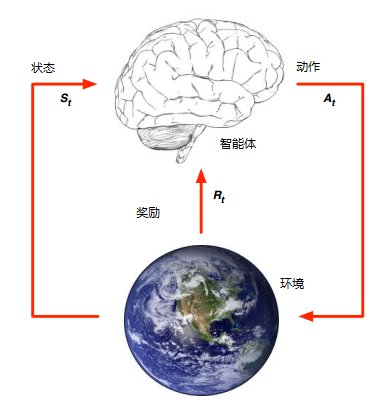
\includegraphics[width=10cm]{example/reinforcement_learning_pro.png}
	\bicaption[强化学习交互过程]
	{强化学习交互过程}
	{Interaction process of reinforcement learning.}
	\label{fig:1}
\end{figure}
\subsection{有限马尔科夫决策过程}
绝大多数强化学习解决的问题都可以抽象为马尔科夫决策过程(Markov Decision Process, MDP)。在决策任务中,对于一个给定的策略,如果环境未来状态的概率分布只取决于当前环境本身,而与历史时刻信息无关,便具有马尔科夫性,其过程成为马尔科夫过程。马尔科夫决策过程由$(S,A,P,R,\gamma )$ 五个元素组成,其中,$S$ 为有限的状态集,$ A $为有限的动作集,$P$ 为状态转移概率,$ R $ 为回报函数,$\gamma$ 为折扣系数。马尔科夫决策过程描述的是这种无记忆的随机过程,可以用下面的状态转移概率公式表达:
\begin{equation}
\label{eq:2}
{P_{ss'}} = P[{S_{t + 1}} = s'|{S_t} = s,{S_{t - 1}},...,{S_1}] = P[{S_{t + 1}} = s'|{S_t} = s]
\end{equation}

其中,$ P $代表状态转移矩阵,包含了所有状态之间转移的概率值:

\begin{equation}
P = \left[ {\begin{array}{*{20}{c}}
	{{P_{11}}}& \cdots &{{P_{1n}}}\\
	\vdots & \ddots & \vdots \\
	{{P_{n1}}}& \cdots &{{P_{nn}}}
	\end{array}} \right]
\end{equation}
$n$为状态的数量。
马尔科夫奖励过程引入了奖励函数$R$和折扣因子$\gamma  \in \left[ {0,1} \right)$,折扣系数代表从当前时刻起对以后获得的所有奖励进行估计,距离当前时刻越远的即时奖励占的比重越小,$\gamma$越接近0,代表从当前状态后向估计越少,$\gamma$越接近1,代表后向估计越多,从某一时刻$0$往后直到当前幕结束所有累计奖励为:
\begin{equation}
\label{eq:resthm}
{{\rm{G}}_{\rm{t}}} = {R_{t + 1}} + \gamma {R_{t + 2}} + ... + \sum\limits_{k = 0}^\infty  {{\gamma ^k}{R_{t + k + 1}}} 
\end{equation}
期望回报表示为:
\begin{equation}
\label{eq:e}
R_{ss'}^a = E[{r_{t{\rm{ + }}1}}{\rm{|}}{{\rm{S}}_t} = s,{S_{t + 1}} = s',{a_t} = a]
\end{equation}
这里引入两个求解MDP问题常用的概念:
\begin{enumerate}
	\item 策略(policy, $ \pi $):策略是智能体面临的决策,由于基于马尔科夫原理,策略只依赖于当前状态,与前面时刻的动作状态无关,因此策略可以表示成一系列二元组:$\left \{ \left ( s_{1},a_{1} \right ),\left ( s_{2},a_{2}\right ),\left ( s_{3},a_{3}\right ),\dots,\left ( s_{n},a_{n}\right )\right \}$。策略可以认为在当前状态下采取某种行动的概率,其完整的表述了智能体的一系列决策过程。
\begin{equation}
\label{eq:3}
\pi (a|s) = P[{A_t} = a|{S_t} = s]
\end{equation}
	\item 值函数(value, v):强化学习建立决策过程是基于对当前状态的评估,称为值函数。值函数为智能体在折扣系数 $\gamma$下的长期累积收益期望。
\end{enumerate}

值函数分为动作值函数$V$ 和状态动作值函数$Q$。在给定状态情况下,对于某一策略 $\pi$, 状态值函数表示直到结束当前过程所获得的累积收益:
\begin{equation}
\label{eq:4}
{v_\pi }(s) = {E_\pi }[{G_t}|{S_t} = s]
\end{equation}
动作值函数指智能体在当前状态下一直遵循策略$ \pi $,采取动作$a$,直到结束当前幕所获得的累积收益:
\begin{equation}
\label{eq:5}
{q_\pi }(s,a) = {E_\pi }[{G_t}|{S_t} = s,{A_t} = a]
\end{equation}
当某一策略的收益期望大于其他策略时,该策略成为最优策略,对应的值函数为最优值函数,最优状态值函数和最后动作-状态值函数表示为:

\begin{equation}
\label{eq:6}
{v_*}(s) = \mathop {\max }\limits_\pi  {v_\pi }(s)
\end{equation}

\begin{equation}
\label{eq:7}
{q_*}(s,a) = \mathop {\max }\limits_\pi  {q_\pi }(s,a)
\end{equation}
根据定理\ref{thm:马尔科夫定理}可知,最优策略总是存在并同时使得状态值函数和状态动作值函数取得最大值。
\begin{thm}[马尔科夫定理]
\label{thm:马尔科夫定理}
对于任意的马尔科夫决策过程:
\begin{enumerate}
	\item 存在一个最优的策略函数${\pi _{\rm{*}}}$使得最后的累积奖励大于其他策略$ \pi$。
	\item 该最优策略函数${\pi _{\rm{*}}}$使得状态值函数达到最大值:
	\begin{equation}
	\label{eq:optimal}
	{v_{{\pi _*}}}(s) = {v_*}(s)
	\end{equation}
	\item 该最优策略函数${\pi _{\rm{*}}}$同时使得状态-动作值函数达到最大值:
	\begin{equation}
	{q_{{\pi _*}}}(s,a) = {q_*}(s,a)
	\end{equation}
	
\end{enumerate}
\end{thm}

求解出最优值函数就解决了马尔科夫决策过程。通常对于状态转移函数已知的模型(model-based),可以通过贝尔曼期望方程求解最优函数:
\begin{equation}
\label{eq:bell1}
{v_\pi }(s) = {E_\pi }[{r_{t + 1}} + \gamma {r_{t + 2}} + {\gamma ^2}{r_{t + 3}} + ...|{S_t} = s] = {E_\pi }[\sum\limits_{k = 0}^\infty  {{\gamma ^k}{r_{t + k + 1}}|{S_t}}  = s]
\end{equation}

将第一步奖励提出来,整理得到:
\begin{equation}
\label{eq:bell3}
{v_\pi }(s) = {E_\pi }[{r_{t + 1}} + \gamma \sum\limits_{k = 0}^\infty  {{\gamma ^k}{r_{t + k + 2}}|{S_t}}  = s]
\end{equation}
其中期望奖励和可以由所有即时奖励累加得到:
\begin{equation}
\label{eq:bell4}
{E_\pi }[\gamma \sum\limits_{k = 0}^\infty  {{\gamma ^k}{r_{t + k + 2}}|{S_t}}  = s] = \sum\limits_a {\pi (s,a)\sum\limits_{s'} {p_{ss'}^a} } \gamma {E_\pi }[\sum\limits_{k = 0}^\infty  {{\gamma ^k}{r_{t + k{\rm{ + }}2}}{\rm{|}}{{\rm{S}}_{t + 1}} = s'} ]
\end{equation}
根据上述公式,方程整理为:
\begin{equation}
\label{eq:bell5}
{V_\pi }(s) = \sum\limits_a {\pi (s,a)\sum\limits_{s'} {p_{ss'}^a} } [R_{ss'}^a + \gamma {E_\pi }[\sum\limits_{k = 0}^\infty  {{\gamma ^k}{r_{t + k + 2}}|{S_{t + 1}}}  = s']]
\end{equation}
利用上一时刻的状态值函数替换\ref{eq:bell5}:
\begin{equation}
\label{eq:bell6}
{V_\pi }(s) = \sum\limits_a {\pi (s,a)\sum\limits_{s'} {p_{ss'}^a} } [R_{ss'}^a + \gamma {V_\pi }(s')]
\end{equation}
同理,动作状态值函数整理为:
\begin{equation}
\label{eq:bell7}
{Q_\pi }(s,a) = \sum\limits_{s'} {p_{ss'}^a} [R_{ss'}^a + \gamma {Q_\pi }(s')]
\end{equation}
相应的,状态值函数和状态动作值函数的最优方程为:
\begin{equation}
\label{eq:bell8}
{V_*}(s) = \mathop {\max }\limits_a \left( {{\rm{R}}_s^a + \gamma \sum\limits_{s' \in S} {P_{ss'}^a{V_*}(s')} } \right)
\end{equation}
\begin{equation}
\label{eq:bell9}
{Q_*}(s,a) = {\rm{R}}_s^a + \gamma \sum\limits_{s' \in S} {P_{ss'}^a\mathop {\max }\limits_{a'} {Q_*}(s',a')}
\end{equation}
\subsection{基于价值函数的算法}
上述方程最优解法都是有模型学习,对于免模型的强化学习可以用基于价值函数的算法求解。典型的基于价值函数求解的算法包括蒙特卡洛(Monte Carlo,MC)\cite{singh1996reinforcement}和时序差分(Temporal-Difference,TD)\cite{tesauro1995temporal}。两种算法都是基于已有的历史数据对价值函数进行更新。

蒙特卡洛是回合制更新,相对更新速度较慢,更新如图\ref{fig:5}。
\begin{figure}[htpb]
	\centering
	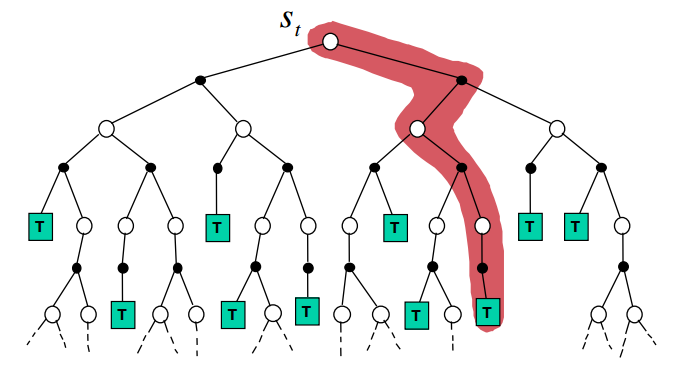
\includegraphics[width=15cm]{example/MC.png}
	\bicaption[蒙特卡洛值函数更新方式示意图]
	{蒙特卡洛值函数更新方式示意图}
	{Monte carlo value function update mode diagram.}
	\label{fig:5}
\end{figure}
MC的更新方式如下:
\begin{equation}
\label{eq:mc}
V({S_t}) \leftarrow V({S_t}) + \alpha [{G_t} - V({S_t})]
\end{equation}
在这里,$\alpha$ 是学习率,也就是更新步长。蒙特卡洛算法通过大量的与环境进行交互获取历史经验信息,通过这些信息近似的估计状态值函数。对于下一次迭代,智能体会根据上一轮的状态值函数选择新的动作,直到收敛。一个典型的蒙特卡洛强化学习算法如\ref{algo:MC}。

\begin{algorithm}
	% \begin{algorithm}[H] % 强制定位
	\caption{蒙特卡洛强化学习算法}
	\label{algo:MC}
	\begin{algorithmic}[1] %每行显示行号
		\State 初始化$Q(s,a) = 0,count(s,a) = 0,\pi (s,a) = \frac{1}{{|A(s)|}}$
		\For {回合$episode = 1 \to N$}
		\State 在环境中执行策略$\pi$,同时记录轨迹$\left\langle {({s_1},{a_1},{r_1}),({s_2},{a_2},{r_2}),...,({s_T},{a_T},{r_T})} \right\rangle  $
		
		\For{$t = 0 \to T-1$}
		\State $R = \frac{1}{{T - t}}\sum\nolimits_{i = t + 1}^T {{r_i}} $
		\State $Q({s_t},{a_t}) = \frac{{Q({s_{\rm{t}}},{a_t}) \times count({s_t},{a_t}) + R}}{{count({s_t},{a_t}) + 1}} $
		\State $count({s_t},{a_t}) = count({s_t},{a_t}) + 1$
		\EndFor
		\State 对于所有已经历过的状态s:
		      
		      策略$\pi (s,a)$更新为$\varepsilon $贪心地选择$\arg {\max _{a'}}Q(s,a')$
		\EndFor
	\end{algorithmic}
\end{algorithm}
在每一次迭代过程中,先让智能体完整的进行一次回合训练,并记录相应的轨迹$\left\langle {({s_1},{a_1},{r_1}),({s_2},{a_2},{r_2}),...,({s_T},{a_T},{r_T})} \right\rangle  $,然后对每一个状态动作对$({s_t},{a_t}) $计算平均累计收益:
\begin{equation}
\label{eq:reward}
R = \frac{1}{{T - t}}\sum\nolimits_{i = t + 1}^T {{r_i}} 
\end{equation}
根据所有累计收益和每个状态访问的次数计算平均收益,这个平均收益就是估计的值函数:
\begin{equation}
\label{eq:reward2}
Q({s_t},{a_t}) = \frac{{Q({s_{\rm{t}}},{a_t}) \times count({s_t},{a_t}) + R}}{{count({s_t},{a_t}) + 1}} 
\end{equation}
TD算法是单步更新制,根据下一时刻奖励$ {R_{t + 1}}$和值函数$V({S_{t + 1}}) $进行当前值函数的更新操作。图\ref{fig:6}为TD算法更新方式。
\begin{figure}[htpb]
	\centering
	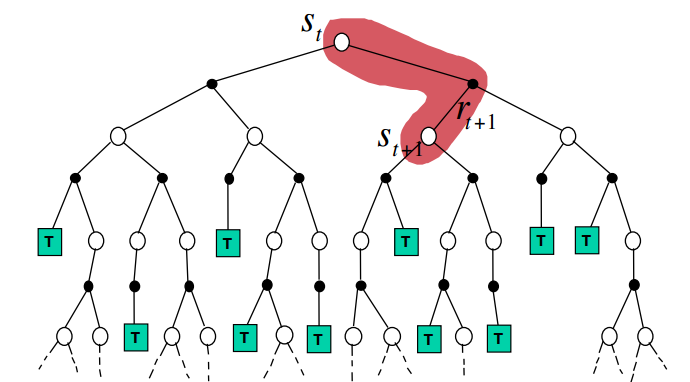
\includegraphics[width=15cm]{example/TD.png}
	\bicaption[单步差分值函数更新方式示意图]
	{单步差分值函数更新方式示意图}
	{Schematic diagram of update mode of single-step difference value function.}
	\label{fig:6}
\end{figure}
TD的更新方式如下:
\begin{equation}
\label{eq:td}
V({S_t}) \leftarrow V({S_t}) + \alpha [{R_{t + 1}} + \gamma V({S_{t + 1}}) - V({S_t})]
\end{equation}
典型的基于TD算法的基于值函数更新的算法有Q-learning算法和Sarsa算法。其算法逻辑分别为算法\ref{algo:Q}和算法\ref{algo:sarsa}。

\begin{algorithm}
	% \begin{algorithm}[H] % 强制定位
	\caption{Q-learning算法}
	\label{algo:Q}
	\begin{algorithmic}[1] %每行显示行号
		\State 初始化$Q(s,a) = 0,\pi (s,a) = \frac{1}{{|A(s)|}},s = {s_0}$
		\For {回合$episode = 1 \to N$}
		\State 输入当前环境状态
		  \For {当前回合没有结束}
		  \State 
		根据当前最新的值函数$Q$和状态$ s $,使用$\epsilon - greddy$策略得到动作$ a $
		  \State 执行动作$ a$,得到即时奖励$r$和新的状态$ s'$
		  \State 更新$ Q $值:$ Q(s,a) \leftarrow Q(s,a) + \alpha [r + \gamma \mathop {\max }\limits_{a'} Q(s',a') - Q(s,a)]$
		  \State 更新状态:$s \leftarrow s'$
		  \EndFor
		\EndFor
	\end{algorithmic}
\end{algorithm}

\begin{algorithm}
	% \begin{algorithm}[H] % 强制定位
	\caption{Sarsa算法}
	\label{algo:sarsa}
	\begin{algorithmic}[1] %每行显示行号
		\State 初始化$Q(s,a)$ = 0
		\Repeat 
		\State 输入当前环境状态
		\State 根据当前最新的值函数$Q$和状态$ s $,使用$\epsilon - greddy$策略得到动作$ a $
		\For {对于当前回合每一步动作}
		\State 执行动作$ a$,得到即时奖励$r$和新的状态$ s'$
		\State 根据当前最新的状态$ s' $,使用$\epsilon - greddy$策略得到新的动作$ a' $
		\State 更新$ Q $值:$ Q(s,a) \leftarrow Q(s,a) + \alpha [r + \gamma Q(s',a') - Q(s,a)]$
		\State 更新状态:$s \leftarrow s'$,:$a \leftarrow a'$
		\EndFor
		\Until{进行完所有的回合数}
	\end{algorithmic}
\end{algorithm}
Sarsa是在线学习方式,根据策略选择出的动作即是最后执行的动作,而Q-learning算法引入了贪心策略,选择Q值最大的动作作为最后执行的动作。

如图\ref{fig:4},TD算法是单步更新,因此更新速率较快,但是由于其更新的目标基于下一步的估计值,更新的方向只取决于下一步的值,估计会带来偏差,因此更新后的价值函数具有高偏差低方差的特性。MC算法是基于回合更新的,其更新的方法取决于本回合所有实际得到的奖励值,因此更新的速度更慢,具有较高的波动,因此MC具有低偏差,高方差的特性。
\begin{figure}[htpb]
	\centering
	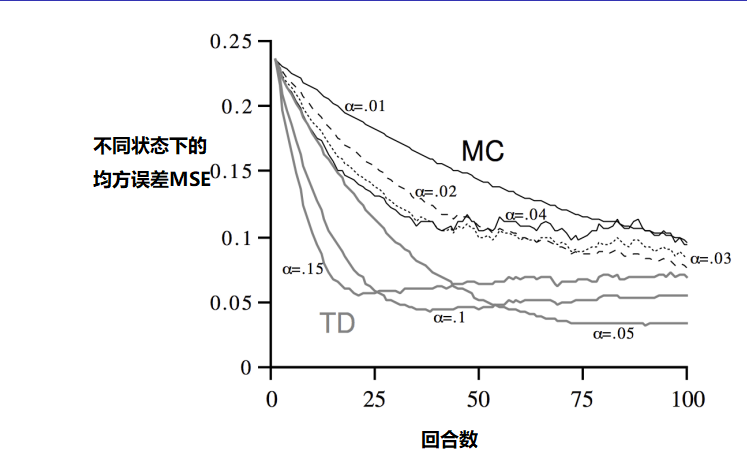
\includegraphics[width=15cm]{example/MC_and_TD.png}
	\bicaption[MC和TD误差随迭代次数变化曲线]
	{MC和TD误差随迭代次数变化曲线}
	{MC and TD errors vary with the number of iterations.}
	\label{fig:4}
\end{figure}
\subsection{基于策略梯度的算法}
和值函数更新的算法进行对比,值函数更新算法是确定性策略算法,一般结合$\varepsilon - greedy$ 算法进行探索避免陷入局部最优,在很多应用场景,动作的选择可能不是唯一的,某几种动作都是合理的,这时候输出所有动作的概率值就会变得更加合理。策略梯度算法最显著的优势是可以防止陷入局部最优解。对于单步的MDP过程来说,从当前状态$S$开始选择一个动作$a$,得到当前状态的即时奖励$ r = R({\rm{s}},a) $,最后的目的是最大化奖励,因此优化的目标函数是$r$本身,即:
\begin{equation}
J(\theta ){\rm{ = }}{{\rm{E}}_\pi }[r] = \sum\limits_{s \in {\rm{S}}} {d(s)\sum\limits_{a \in A} {\pi (a|s;\theta )} } R(s,a)
\end{equation}
其中${\pi (a|s;\theta )}$是参数为$\theta$的策略网络。对目标函数求导:
\begin{equation}
\begin{split}
{\nabla _\theta }J(\theta ) =& \sum\limits_{s \in S} {d(s)\sum\limits_{a \in {\rm{A}}} {\pi (a|s;\theta )} } \frac{{{\nabla _\theta }\pi (a|s;\theta )}}{{\pi (a|s;\theta )}}R(s,a) \\
=& \sum\limits_{s \in S} {d(s)\sum\limits_{a \in {\rm{A}}} {\pi (a|s;\theta )} } {\nabla _\theta }\log \pi (a|s;\theta )R(s,a) \\
=& {E_\pi }[{\nabla _\theta }\log \pi (a|s;\theta )R(s,a)]
\end{split}
\end{equation}
最后目标函数的梯度由两部分组成,一部分是策略函数对数梯度和即时奖励两部分乘积的期望值。以上是单步MDP过程的求解过程,对于多步MDP:
\begin{equation}
{\nabla _\theta }J(\theta ) = {E_\pi }[{\nabla _\theta }\log \pi (a|s;\theta ){Q_\pi }(s,a)]
\end{equation}
同样,基于策略梯度算法的强化学习也可以采用蒙特卡洛方法进行求解。也称为REINFORCE算法\cite{williams1992simple}。如算法\ref{algo:REINFORCE}所示。

\begin{algorithm}
	% \begin{algorithm}[H] % 强制定位
	\caption{REINFORCE算法}
	\label{algo:REINFORCE}
	\begin{algorithmic}[1] %每行显示行号
		\State 初始化网络参数$ \theta$ 
		\For {对于每一回合根据当前策略$\pi$得到走过每一步的$\{ {s_0},{a_0},{r_1},...,{s_{T - 1}},{A_{T - 1}},{R_T}\} $}
		\For{$t = 0 \to T-1$}
		\State 更新参数:$ \theta  \leftarrow \theta  + \alpha {\nabla _\theta }{G_t}\log \pi ({A_t}|{S_t};\theta )$
		\EndFor
		\EndFor
	\end{algorithmic}
\end{algorithm}

以上是传统强化学习的三种求解算法,对于复杂场景,对于外界环境的感知和特征提取能力显得尤为重要,对于函数拟合部分也越发变得困难,由此衍生了将强化学习模型和深度学习模型结合的深度强化学习模型。
\section{深度强化学习常见算法模型}
正如上文所述,对于免模型学习,强化学习最优方程的求解可以有基于价值网络和基于策略梯度以及结合价值网络和策略梯度同时进行求解的算法。结合深度学习模型也相应的延生出了两种基本的深度强化学习模型。下面分别介绍这两种算法。
\subsection{Deep Q-learning算法介绍}
作为离线学习的值函数更新方法,Q-learning学习方法被广泛用于不同强化学习场景。Q-learnig中状态动作价值函数$Q(s,a)$通常以表格的形式给出来。如图\ref{fig:8},行代表不同的状态,列代表在对应状态下可选择的动作。
\begin{figure}[htpb]
	\centering
	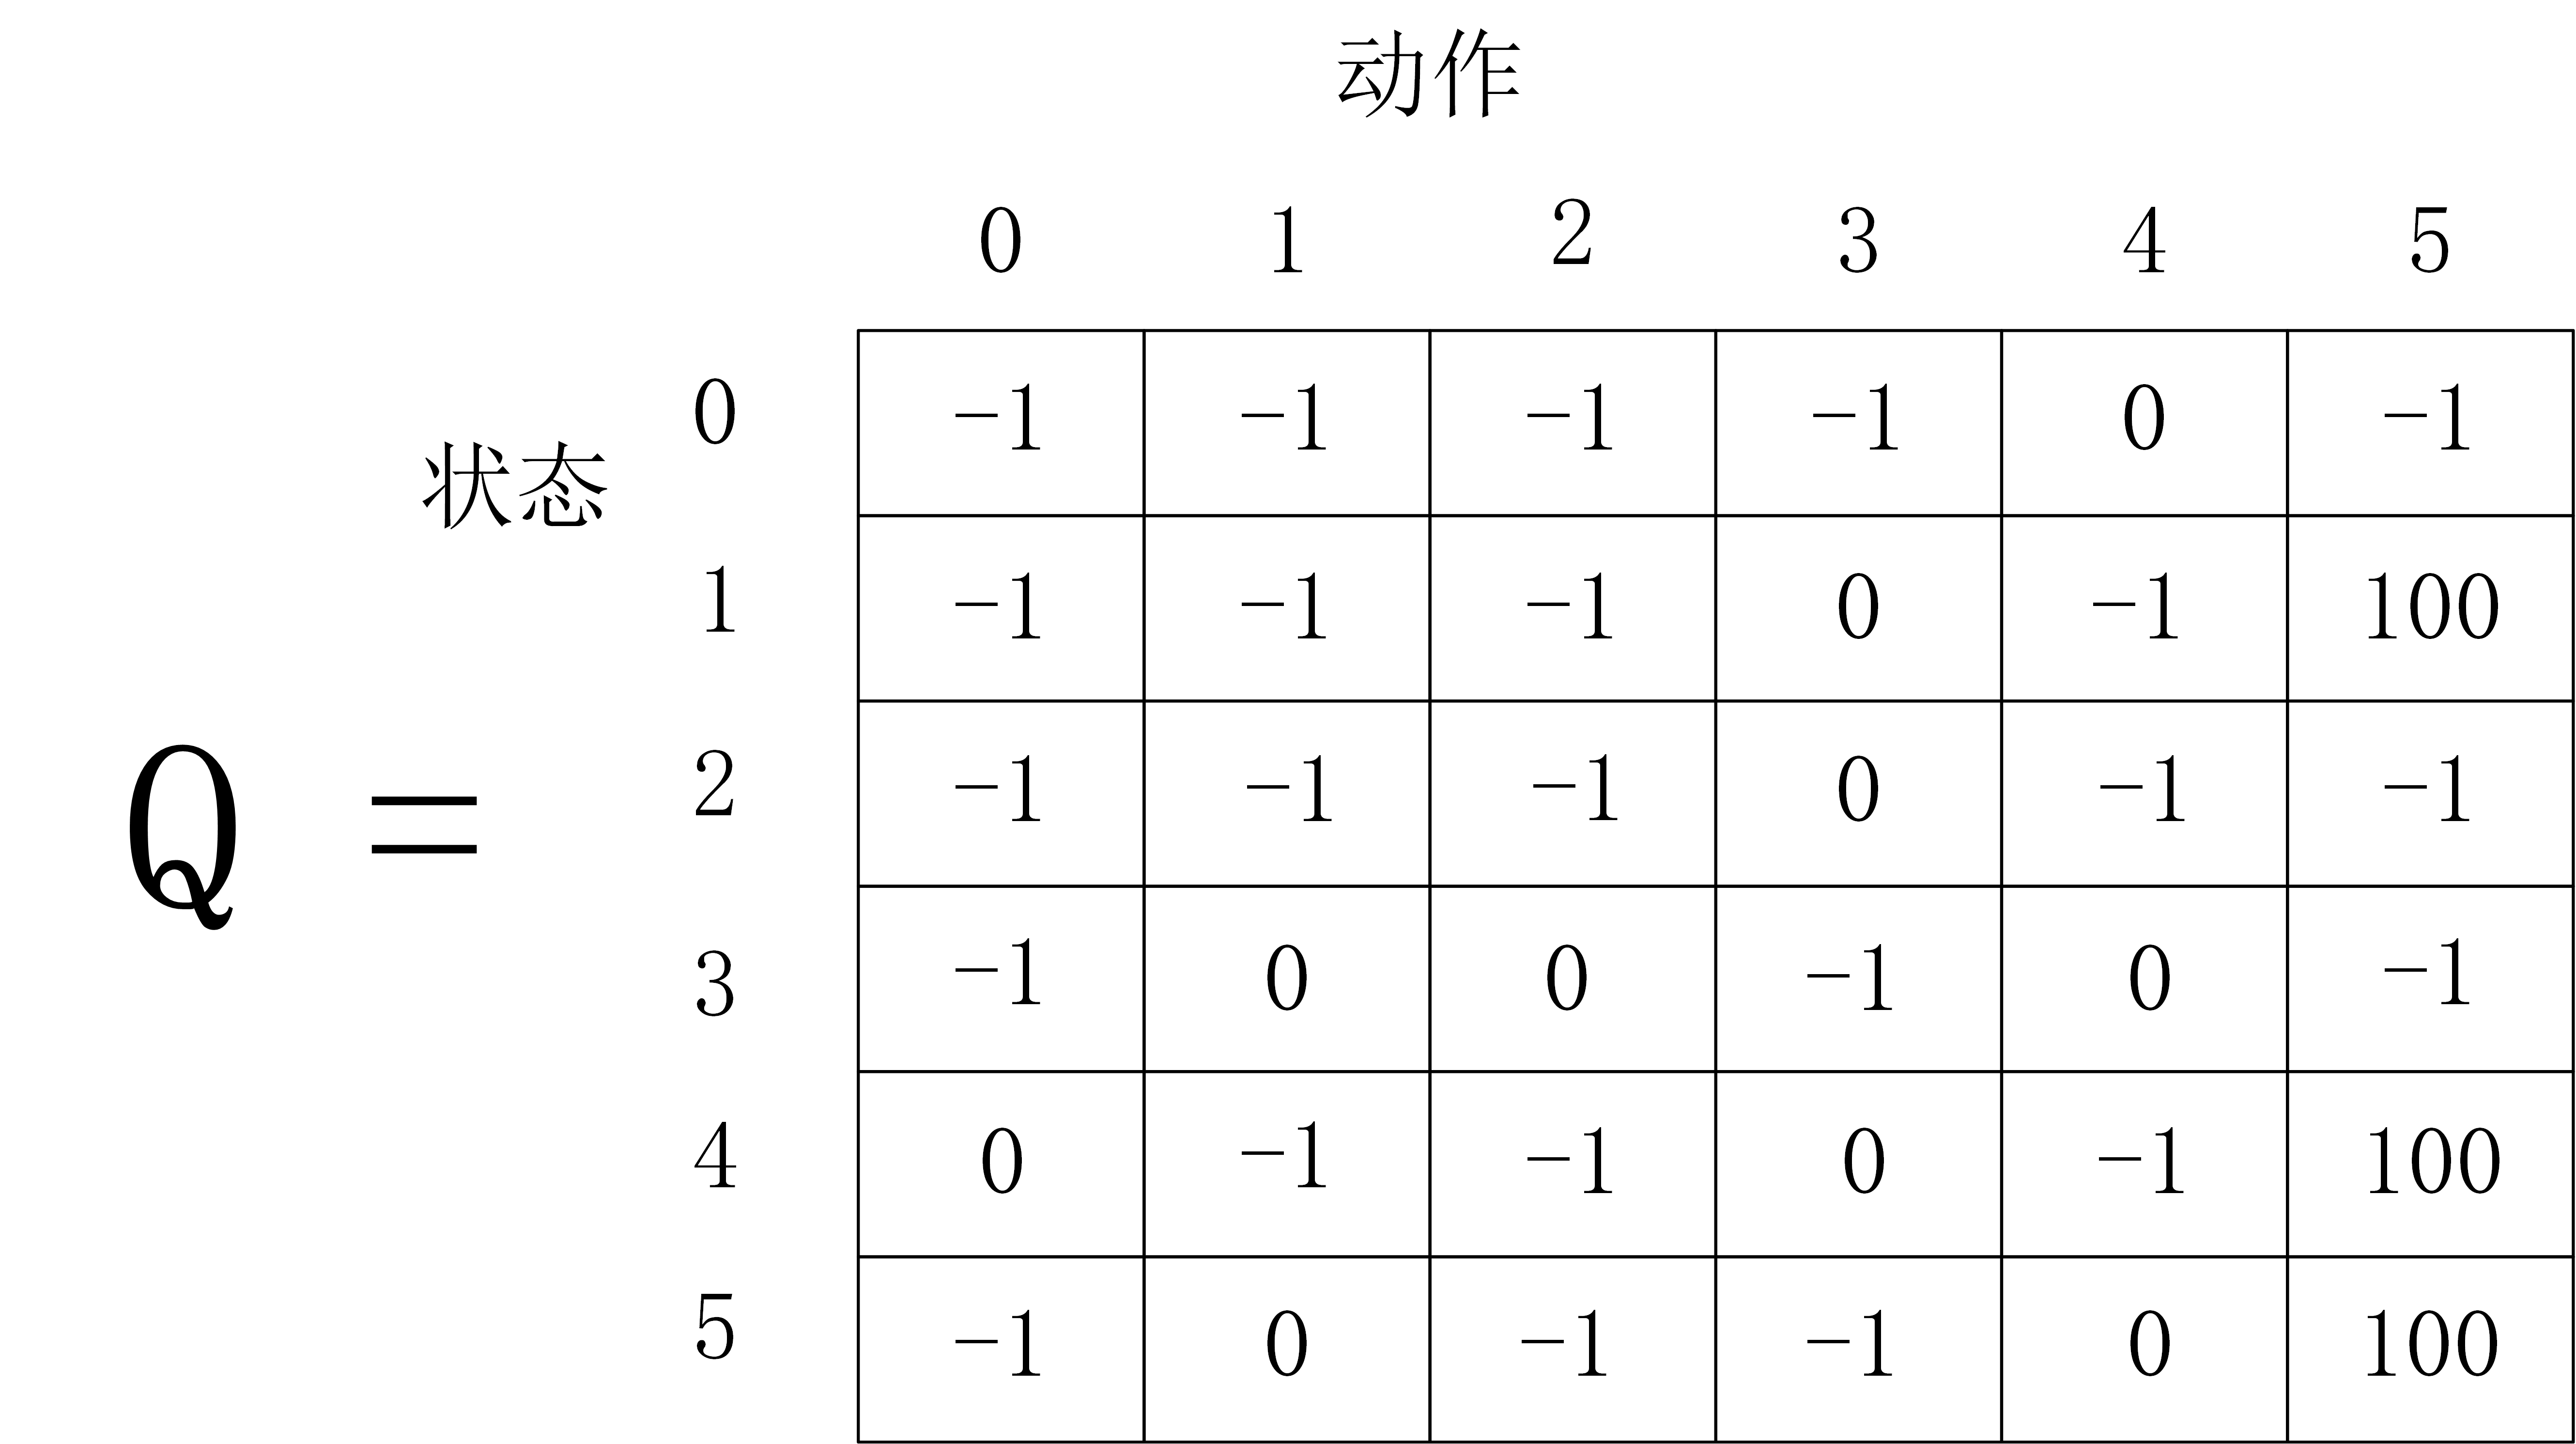
\includegraphics[width=\hsize]{example/Q_table.jpg}
	\bicaption[Q值表示意图]
	{Q值表示意图}
	{The Q table.}
	\label{fig:8}
\end{figure}
从上一节介绍可知,随着环境复杂度和动作可选范围增加,状态空间和动作空间的笛卡尔积尺寸变大,需要优化的状态动作值函数计算复杂度呈指数级数增长。对于高维的环境特征信息,如在图像视频领域,Q-learning算法不再适用,将深度学习网络应用在Q-learning框架下作为价值函数的逼近器代替传统的Q表想法应运而生,这种算法就是深度Q价值网络(Deep Q-learning,DQN)。DQN算法可以直接从原始输入状态中学习环境特征,返回值函数。用深度学习网络输出值近似逼近Q值函数:
\begin{equation}
	{\rm{Q}}(s,a) \approx Q(s,a;\theta )
\end{equation}
其中,$\theta $为深度学习网络参数。DQN网络参数更新公式为:
\begin{equation}
\label{eq:DQN}
L(\theta ) = \frac{1}{2}{(y - Q(s,a;\theta ))^2}
\end{equation}
$y$为神经网络拟合的标签信息,对应于Q-learning中对目标的估计:
\begin{equation}
y = r + \gamma {\max _{a'}}Q({\rm{s'}},a';\theta )
\end{equation}
带入式\ref{eq:DQN}:
\begin{equation}
\label{eq:DQN2}
	{\nabla _\theta }L(\theta ) = (r + \gamma \mathop {\max }\limits_{a'} Q(s',a';\theta ) - Q(s,a;\theta )){\nabla _\theta }Q(s,a;\theta )
\end{equation}
在数据存储方面,DQN引入了经验回放技术,提高了样本的利用率,一定程度上减少了计算机的负担。每一个时刻智能体与环境交互产生的数据$ \left\langle {{s_t},{a_t},{r_{t + 1,}}{{\rm{s}}_{t + 1}}} \right\rangle $ 都存储在经验池中,在深度学习网络训练过程中每次参数的更新都会随机从经验池中采样出一个小批量样本进行学习。之后智能体再次采用随机-贪心算法进行动作的选择,DQN的算法如算法\ref{algoDQN}所示。

\begin{algorithm}
	% \begin{algorithm}[H] % 强制定位
	\caption{DQN算法}
	\label{algoDQN}
	\begin{algorithmic}[1] %每行显示行号
		\State 初始化Q网络参数更新的频率$C$,Q网络的参数$\theta$,最终输出目标网络参数$\theta ' = \theta $
		\For {回合数从1到$ M $}
		\State 初始化状态$ {s_1}$
		\For {动作步数从1到时刻$ T$}
		\State 根据当前最新的状态$ {s_t}$,使用$\epsilon - greddy$策略得到新的动作$a_t $
		\State 执行$a_t $,获取最新的奖励$ r_t+1 $,到达新的状态$ {s_t+1}$
		\State 将收集到的状态动作和奖励数据$ \left\langle {{s_t},{a_t},{r_{t + 1,}}{{\rm{s}}_{t + 1}}} \right\rangle $存储在经验池中
		\State 从经验池中随机采样mini-batch大小的数据$ \left\langle {{s_j},{a_j},{r_{j + 1,}}{{\rm{s}}_{j + 1}}} \right\rangle $,对于每一条数据计算估计Q值$y$:$ {y_j} = \left\{ {\begin{array}{*{20}{c}}
			{{{\rm{r}}_j}{\rm{,end}}}\\
			{{r_j} + \gamma \mathop {\max }\limits_{a'} \hat Q({s_{j + 1}},a';\theta '),not}
			\end{array}} \right.$
		\State 以公式\ref{eq:DQN2}为损失函数,对网络参数进行梯度下降更新。
		\State 以C为更新频率进行网络权重的更新$\theta ' = \theta $。
		\EndFor
		\EndFor
	\end{algorithmic}
\end{algorithm}
\subsection{Actor-Critic策略梯度算法}
蒙特卡洛策略梯度算法通过每一回合的完整更新,计算出来累积奖励价值往往相对准确,但是方差较大。值函数引导策略的更新,策略同时影响值函数的更新,这样两者循环训练,学习的效果会有所提升,这就是演员-评论家模型(Actor-Critic,AC)。

这里引入优势函数(advantage function)的概念,优势函数代表当智能体在$t$时刻采取$a_t$ 动作后达到的状态要比当前状态$s_t$的总体平均价值提升程度,公式表示为:

\begin{equation}
{A_\pi }(s,a) = {Q_\pi }(s,a) - {V_\pi }(s)
\end{equation}
Actor-Critic模型的损失函数可以引入优势函数:
\begin{equation}
\label{eq:ac}
J(\theta ) = {E_\pi }[\log \pi (a|s;\theta ){A_\pi }(s,a)]
\end{equation}
这里${V_\pi } $和$ {Q_\pi } $利用TD更新优势函数,把动作状态值函数转化为状态值函数,优势函数的TD误差变为:
\begin{equation}
\label{eq:error}
{\delta _\pi } = r + \gamma {V_\pi }(s') - {V_\pi }(s)
\end{equation}
利用\ref{eq:error}公式更新策略网络梯度式\ref{eq:ac}:
\begin{equation}
{\nabla _\theta }J(\theta ) = {\nabla _\theta }\log \pi (A|s;\theta )(r + \gamma V(s';{\theta _v}) - V(s;{\theta _v})) = \delta {\nabla _\theta }\log \pi (A|s;\theta )
\end{equation}

\begin{figure}[htpb]
	\centering
	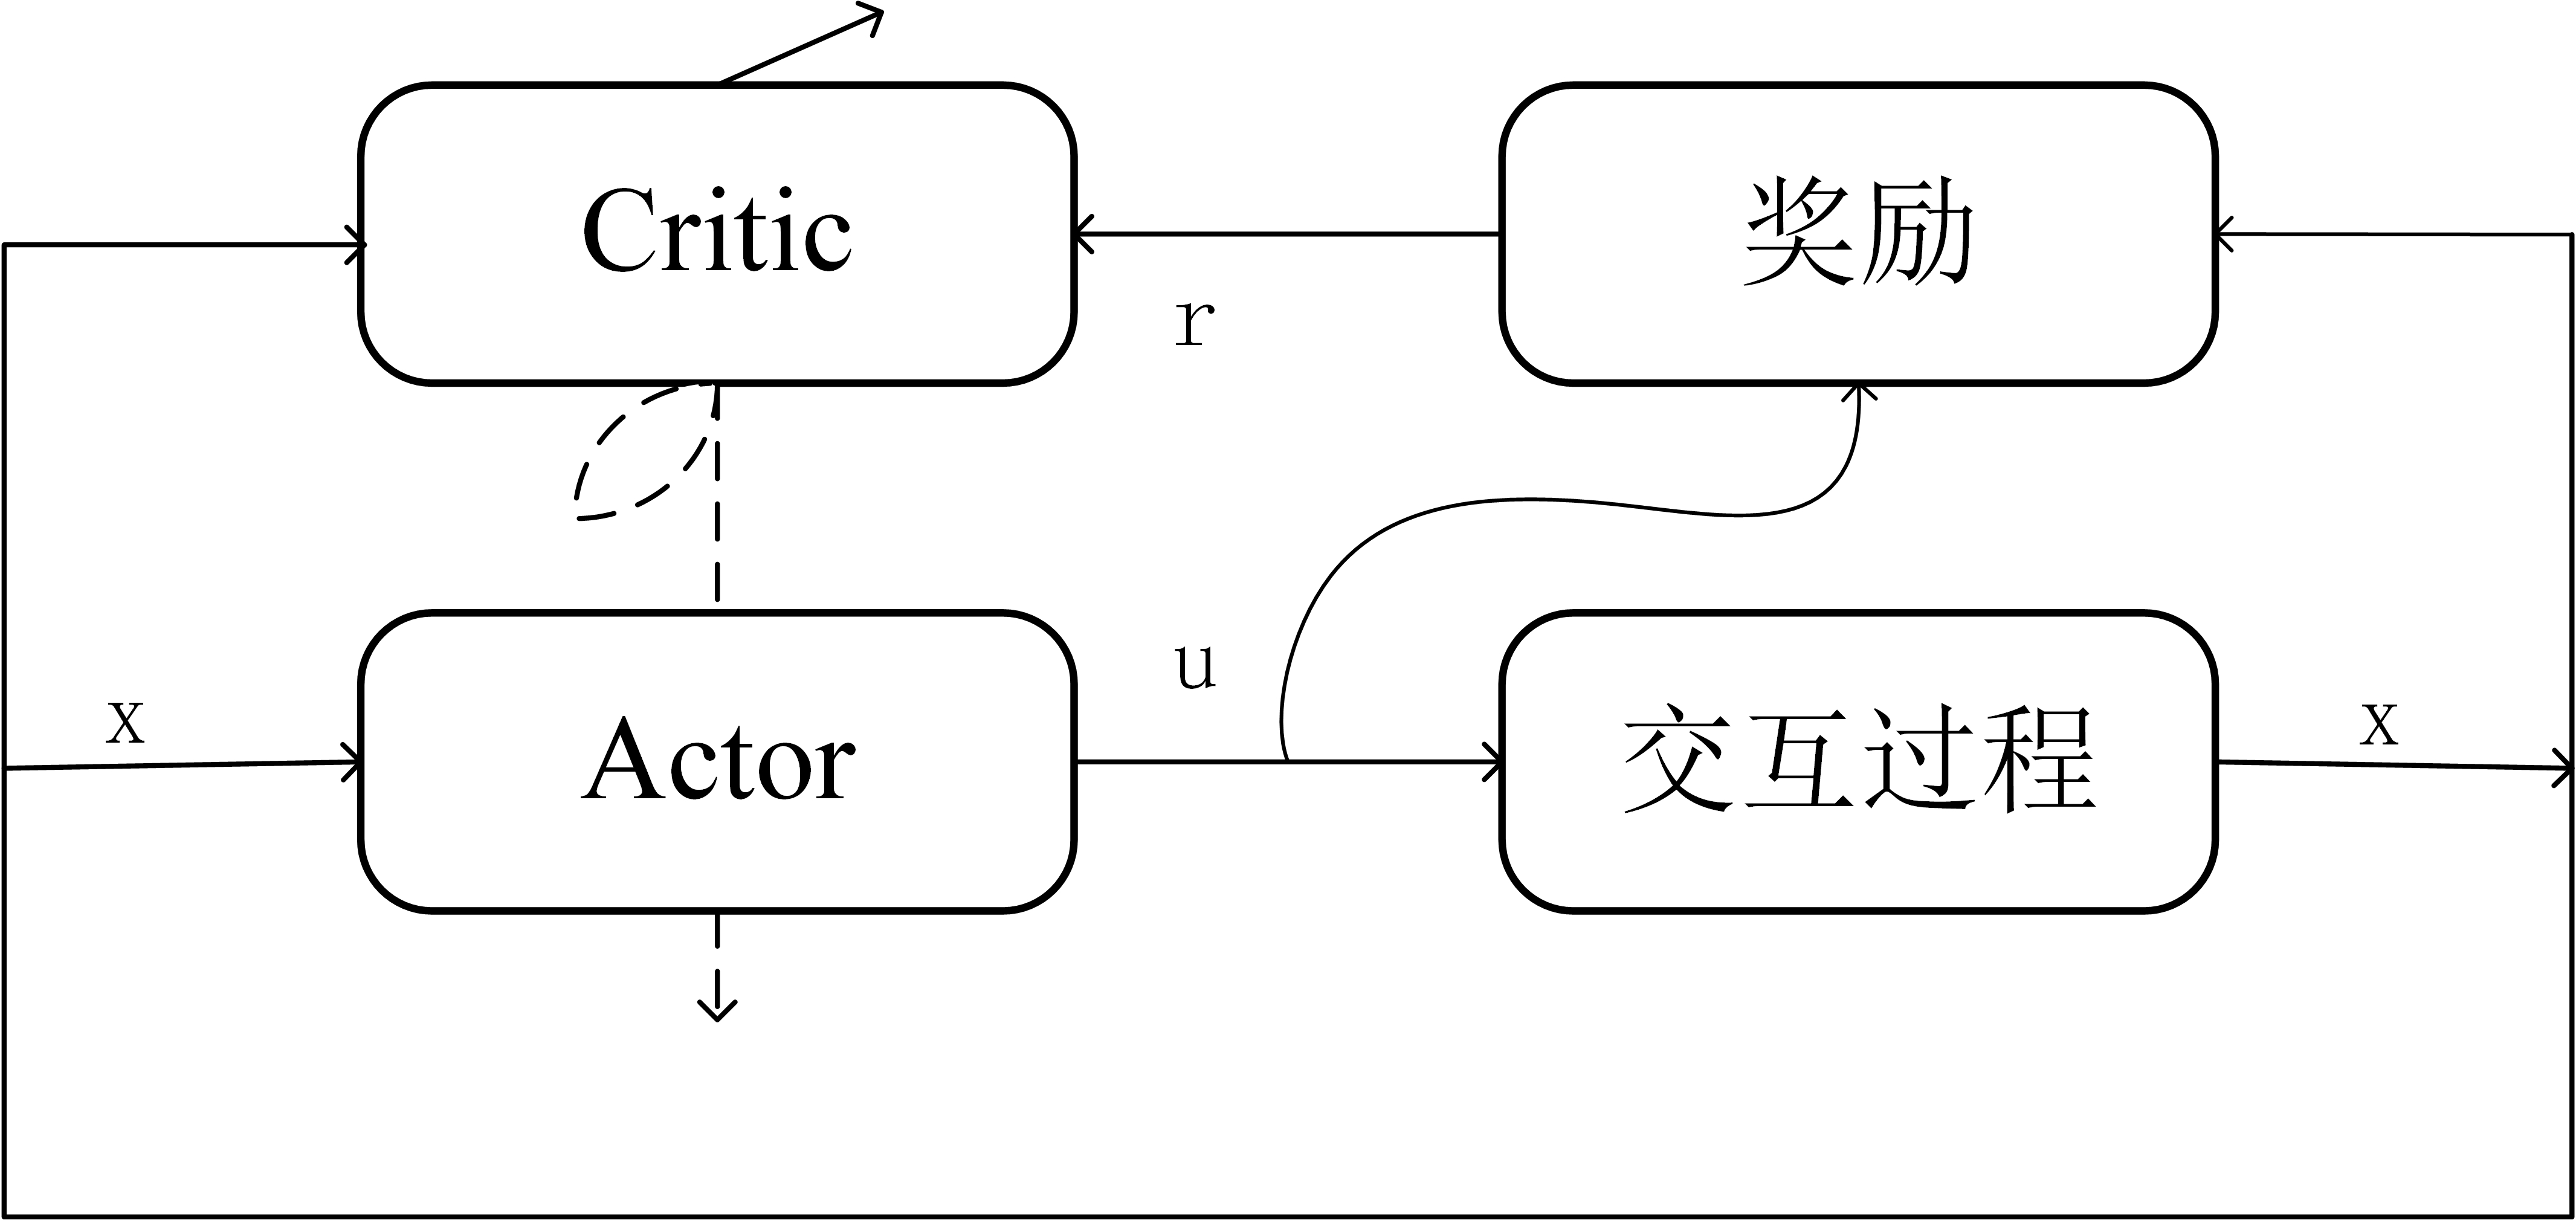
\includegraphics[width=\hsize]{example/ac.jpg}
	\bicaption[Actor-Critic策略梯度算法更新过程]
	{Actor-Critic策略梯度算法更新过程}
	{Actor-critic policy gradient algorithm update process.}
	\label{fig:ac}
\end{figure}
如图\ref{fig:ac}所示,Actor-Critic模型由两个部分组成:Actor基于动作概率选择下一步的动作,Critic根据当前的状态和Actor选择的动作获得的数据进行采样,逼近值函数进行打分,在下一次迭代中,Actor又会根据Critic打分值沿着最大化收益的方向改变动作概率输出。相对于传统的值函数更新,AC模型引入了策略梯度进行智能体策略的监督,使得训练更加稳定,同时AC模型利用TD方法进行优化函数的更新,弥补了蒙特卡洛策略梯度回合制更新方差大训练时间长的不足。AC模型的算法过程如算法\ref{algo:DQN}。
\begin{algorithm}[htbp]
	% \begin{algorithm}[H] % 强制定位
	\caption{Actor-Critic策略梯度算法}
	\label{algo:DQN}
	\begin{algorithmic}[1] %每行显示行号
		\State 初始化策略网络参数和价值网络参数
		\For {回合数从1到$ M $}
		\State 初始化状态$ {s}$
		\For {动作步数从1到时刻$ T$}
		\State 根据当前最新的状态$ {s}$作为策略网络的输入,策略网络的输出为动作概率分布,依概率选择一个动作$ a_t $
		\State 执行$a_t $,获取最新的奖励$ r_t+1 $,到达新的状态$ {s'}$
		\State 计算TD误差${\delta _\pi } = r + \gamma {V_\pi }(s') - {V_\pi }(s)$
		\State 更新状态价值网络:${\theta _v} \leftarrow {\theta _v} + \beta \delta {\nabla _{{\theta _v}}}V(s;{\theta _v})$,其中,$\beta$ 为学习率
		\State 更新策略网络:$\theta  \leftarrow \theta  + \alpha \delta {\nabla _\theta }\log \pi (A|s;\theta )$,其中,$\alpha$ 为学习率
		\State 更新状态:$ s \leftarrow s'$
		\EndFor
		\EndFor
	\end{algorithmic}
\end{algorithm}

\section{本章小结}
本章第一部分首先介绍了强化学习了理论基础知识,与监督学习和无监督学习进行了对比,接下来介绍了强化学习基本的组成,强化学习中智能体和环境的交互过程,对于马尔可夫过程的求解,有两种方式,一种是回合更新制的蒙特卡洛算法,一种是单步更新的差分算法。根据强化学习动作选择的依据又可以分为基于值函数的强化学习和基于策略梯度的强化学习。基于值函数更新的强化学习算法主要基于状态值函数或者状态动作值函数对当前时刻状态进行评分,然后确定下一步动作的选择。常用的值函数更新的强化学习包括在线学习的Sarsa算法和离线学习的Q-learning算法。基于策略梯度更新算法,主要根据当前状态输出可行动作的概率值,对于连续型决策任务尤为有效,传统的基于策略梯度更新的强化学习中主要为REINFORCE算法,对于单步更新和多步更新的过程文中都有相应介绍。本章的第二部分引入了深度强化学习的概念,深度强化学习结合了深度学习的感知和特征提取能力和强化学习的决策能力,这一部分主要介绍了两种深度强化学习的算法:DQN算法和Actor-Critic算法。DQN在Q-learning算法的基础上,把传统的Q表替换为深度学习网络,深度学习作为函数的逼近器具有更强的泛化能力和函数拟合的能力,数据经验池的引用消除了数据时间上的关联性,同时增加了数据的利用效率。Actor-Critic策略梯度算法结合了值函数更新算法可以准确估计当前状态评分和策略梯度下降法能够有效使用TD算法进行连续快速更新的优势。
本章在介绍强化学习基础知识后详细介绍了5种常用的算法并剖析不同算法的利弊,为后续章节奠定了理论基础。

%# -*- coding: utf-8-unix -*-
% !TEX program = xelatex
% !TEX root = ../thesis.tex
% !TEX encoding = UTF-8 Unicode
%%==================================================
%% chapter01.tex for SJTU Master Thesis
%%第三章
%%==================================================
\chapter{有监督信号的WGAN网络对数据的扩充}
生成式对抗网络(Generative adversarial networks,GAN)\cite{Goodfellow2017NIPS}是深度强化学习应用在数据生成上的成功案例。近年来生成式对抗网络在很多领域有了良好的应用,如:图像合成,图像修补,图像着色,视频预测,文字图像生成,等等。但是生成式对抗网络在其他非图像类领域应用的场景有待发展,其次生成式对抗网络由于损失函数本身是极小极大化的过程,因此纯在训练不稳定,生成样本覆盖不均的缺点。本章将分别介绍原始生成式对抗网络及其发展,并针对特定数据和现有问题提出改进算法原理及方案。
\section{引言}

众所周知,机器学习模型可以根据其学习到的数据形式分为生成式模型(Genenrative Model)和判别式模型(Discriminative Model)。判别式模型是基于决策函数$Y = f(X) $ 或者条件概率分布$ P(Y|X)$进行建模的,判别模型关心的是对于给定的输入$X$ 应该预测出什么样的输出$Y$,输入的数据是原始特征信息,输出的是每条样本对应的标签值。生成式模型由数据学习联合概率分布$P(X,Y)$,然后求条件概率分布$P(Y|X)$作为预测模型,也就是$P(Y|X) = \frac{{P(X,Y)}}{{P(X)}}$,生成式模型可以同时产生样本的特征值及其对应的标签信息\cite{Generative or discriminative? getting the best of both worlds}。典型的判别模型包括:K近邻法\cite{Hartigan1979Algorithm},感知机,决策树,逻辑斯谛回归模型,最大熵模型,支持向量机,提升方法,和条件随机场,等等。在这里我们研究的是小数据集样本的数据扩充,所以用到的是生成式模型,利用极大似然估计算法的深度生成式模型根据其表示或估计似然的方式不同,有很多分类方法\cite{bibid}如图\ref{fig:生成式模型分类树状图}所示。根据似然估计过程基于的函数类型可以将生成模型分为显示密度函数和隐式密度函数,基于显示密度函数的经典算法有PicelRNN\cite{Oord2016Pixel}和变分自编码器\cite{Kingma2013Auto},基于隐式密度函数经典算法有马尔科夫链和生成式对抗网络等等。

\begin{figure}[htpb]
	\centering
	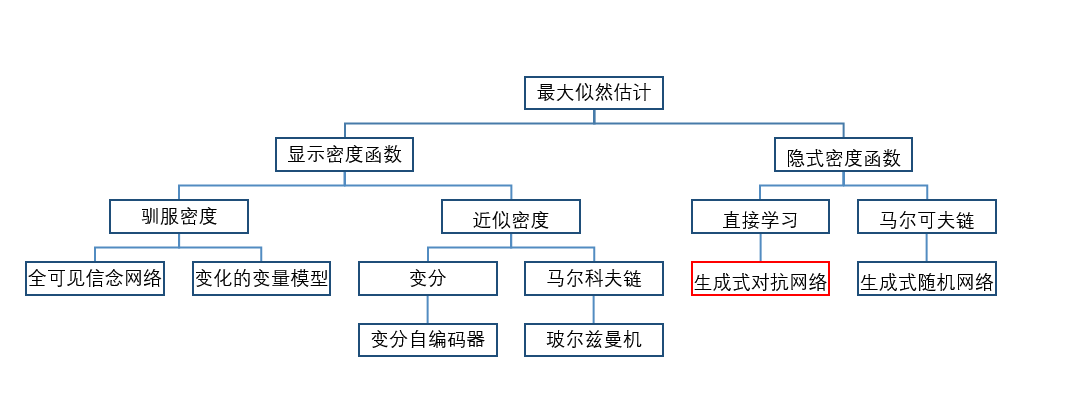
\includegraphics[width=15cm]{example/generate.png}
	\bicaption[这里将出现在插图索引]
	{生成式模型分类树状图}
	{Generated model classification tree graph}
	\label{fig:生成式模型分类树状图}
\end{figure}

在实际问题中,大量样本数据往往很难获得或获取成本较高,而通常情况下在深度学习领域模型又是依赖于大量样本进行学习的,因此对于小样本数据集要想更好的学习数据分布的规律,就需要进行数据增强,在图像领域,常用的数据扩充方法有图像的翻转,旋转,尺度尺度变换,随机抠取,色彩抖动等等,在机器学习领域,常用的方法有Fancy PCA\cite{Holdt2010Genome},监督式抠取,以及我们接下来主要研究的生成式对抗网络的生成方法。数据增强一方面通过增加更多的数据提供信息提高了模型的泛化能力,另一方面引入了更多的噪声数据,能提高模型的鲁棒性。如果数据的分布可以用过模型利用概率统计的方式表达出来,那么产生更多的符合该概率分布的数据就达到了数据增强的目的。本章节主要介绍了生成式对抗网络的基本原理及改进算法,并针对实验数据类型对网络模型引入了监督信息,提高了模型的有效性。
\section{GAN算法}
\subsection{GAN基本框架}
生成式对抗网络于2014年被蒙特利尔大学的Goodfellow Ian首次提出, 由于其出色的表现,引起了业界学者的广泛关注。当强化学习的任务是对样本进行增强时,是通过生成式对抗网络进行实现的。作为Actor-Critic框架下的一员,生成式对抗网络主要有两个部分组成:生成器(Generator)和判别器(Discriminater)。生成器是生成式模型,主要学习数据的联合概率分布,图\ref{fig:生成式模型分类树状图}示意了GAN两个组成部分之间的关系。

\begin{figure}[!htp]
	\centering
	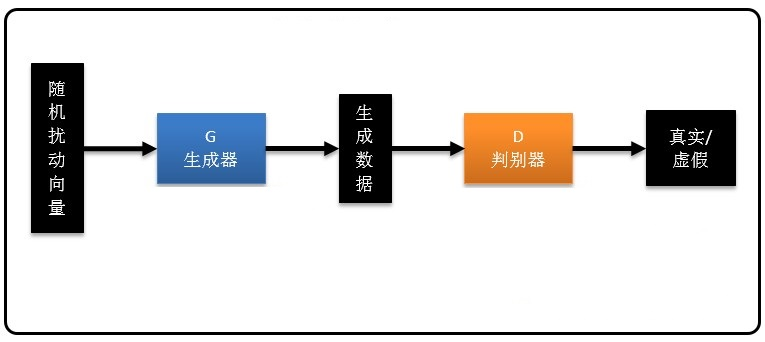
\includegraphics[width=10cm]{example/GAN1.jpg}
	\hspace{1cm}
	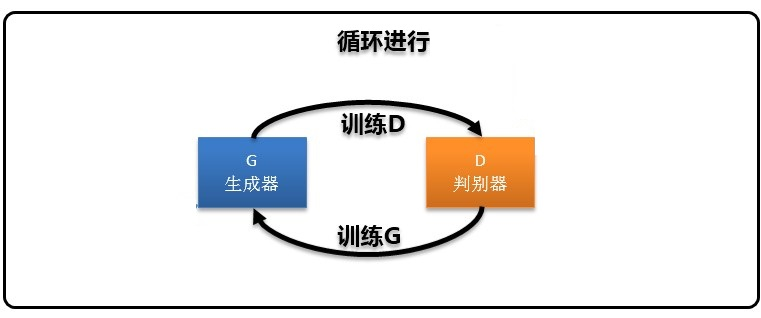
\includegraphics[width=10cm]{example/GAN2.jpg}
	\bicaption[这里将出现在插图索引中]
	{GAN结构示意图}
	{Framework of GAN}
	\label{fig:GAN1}
\end{figure}
其输入的数据为任意形式的噪声,输出的数据为学习到的假样本,判别器相当于一个二分类模型,其输入的数据为原始真实数据和生成器生成的假数据,输出的是输入样本属于真实样本的概率,概率值越大,代表该样本是真实样本的概率越大。生成式利用零和博弈模型把生成式模型和判别式模型整合在了一个框架下。对应于强化学习,GAN里面的生成器相当于智能体,生成器生成的数据就是智能体进行的动作,判别器相当于环境反馈的奖励,当生成的数据越接近真实数据,奖励值越大,生成器会向着该方向更新参数,反之当生成的数据离真实样本分布越远,奖励越小,生成器参数向反方向更新。在这里面,生成器和判别器可以是任何框架下的模型,通常在应用中都使用深层神经网络进行生成器和判别器的构造。

\subsection{GAN算法介绍}
GAN作为生成式模型,求联合概率密度函数离不开极大似然估计,似然估计函数如式\ref{eq:EM}:

\begin{equation}
\label{eq:EM}
\max \limits_{\theta\in R^{d}}\frac{1}{m} \sum_{i=1}^m \log P_{\theta}(x^{(i)})
\end{equation}
在这里,$P_{\theta}$ 是密度函数的参数, $\{x^{(i)}\}^{m} _{i=1}$是从真实数据中采样得到的采样数据。
生成式对抗网络的优化目标函数可以用\ref{eq:22}函数描述。
\begin{equation}
\label{eq:22}
G^{*}=\arg \min \limits_{G} \max \limits_{D} V(G,D)
\end{equation}
这里:
\begin{equation}
\label{eq:33}
V=E_{x\sim P_{data}} [\log D(x)]+E_{x\sim P_{G}}[\log (1-D(x))]
\end{equation}
其中,$P_{data}$代表真实数据的分布,$P_{G}$ 代表生成器学习 $G$得到的假的数据的分布。 $D$ 代表判别器。当我们确定生成器和判别器都是神经网络时,用${\theta _g}$和${\theta _p}$ 分别代表生辰器和判别器的网络结构参数。生成器是可微的。定义输入的噪声数据为$ {p_z}(z)$,可以用${\rm{G(z,}}{\theta _g}{\rm{)}}$表示生成器对数据从噪声分布到学习到数据分布的映射关系。$D(x,{\theta _d})$输出单变量代表概率值。\ref{eq:33}整理为:
\begin{equation}
\label{eq:44}
\mathop {\min }\limits_G \mathop {\max }\limits_D v(D,G) = {E_{x \sim {p_{data}}(x)}}[\log D(x)] + {E_{z \sim {p_z}(z)}}[\log (1 - D(G(z)))]
\end{equation}
 这是一个极小极大化的损失函数,对于一个固定的$G$,对$D$求解其最优函数:
 \begin{equation}
 \label{eq:34}
 {D^*}(x) = \frac{{{p_{data}}(x)}}{{{p_{data}}(x) + {p_g}(x)}}
\end{equation}
 类似地,对于固定的$G$,求$D$的目标是最大化损失函数
\begin{equation}\label{eq:36}
\begin{split}
v(G,D) =& \int_x {{p_{data}}(x)\log (D(x))}\mathrm{d}x + \int_z {{p_z}(z)\log (D(z))}\mathrm{d}x  \\
=&  \int_x \bigg( {{p_{data}}\log ({\rm{D}}(x)) + {p_g}(x)\log (1 - D(x))\bigg)}\mathrm{d}x 
\end{split}
\end{equation}
所以\ref{eq:33},\ref{eq:22}可以整理为:
\begin{equation}
\label{eq:35}
\begin{split}
\mathop {\max }\limits_D v(G,D) =& {E_{x \sim {p_{data}}}}[\log {D^*}_G(x)] + {E_{x \sim {p_g}}}[\log (1 - {D^*}_G(x))] \\
=& {E_{x \sim {p_{data}}}}[\log \frac{{{p_{data}}(x)}}{{{p_{data}}(x) + {p_g}(x)}}] + {E_{x \sim {p_g}}}[\log \frac{{{p_{data}}(x)}}{{{p_{data}}(x) + {p_g}(x)}}]
\end{split}
\end{equation}
整理后得到:
\begin{equation}
\label{eq:37}
\mathop {\max }\limits_D v(G,D) =  - \log 4 + KL({p_{data}}||\frac{{{p_{data}} + {p_g}}}{2}) + KL({p_g}||\frac{{{p_{data}} + {p_g}}}{2})
\end{equation}
其中$KL$ 项表示$KL$散度\cite{joyce2011kullback},是衡量两个数据分布之间距离的函数。整理成$ JS $ 散度衡量变成:
\begin{equation}
\label{eq:38}
\mathop {\max }\limits_D v(G,D) =  - \log 4 + 2JSD({p_{data}}||{p_g})
\end{equation}

可以证明当生成器和判别器的有足够的泛化拟合能力时,对于固定的生成器,判别器都可以达到最优,然后最大化$\mathop {\max }\limits_D v(G,D) = {E_{x \sim {p_{data}}}}[\log {D^*}_G(x)] + {E_{x \sim {p_g}}}[\log (1 - {D^*}_G(x))]$ 求最优的生成器。最后$P_g$将收敛于$p_data$。这样,损失函数可以理解为判别器希望生成的假数据和原始数据分布之间的距离越大越好,而生成器希望两个数据之间的分布越接近越好。GAN训练过程的示意图如\ref{fig:train}所示。

\begin{figure}[htpb]
	\centering
	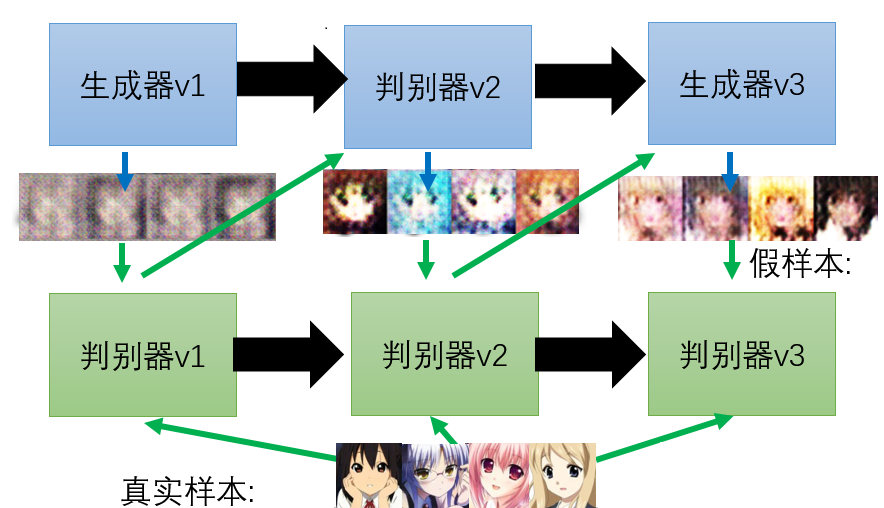
\includegraphics[width=15cm]{example/GAN3.png}
	\bicaption[这里将出现在插图索引]
	{GAN训练过程图示}
	{Generated model classification tree graph}
	\label{fig:train}
\end{figure}

先随机初始化生成器和判别器参数,生成器$v1$生成初始版本假数据连同真实数据一起作为判别器$V1$的输入,判别器$v1$把判别结果送给$v2$生成器,给$v2$生成器打分指导其参数更新的方向。然后$v2$生成器生成新的一批假数据,在这里给真实数据打标签为1,假数据打标签为0,两种数据一起作为判别器$v2$训练的样本数据,循环以上过程,直到整个网络达到一个相对稳定的状态。
算法描述如下:

\begin{algorithm}[!h]
	\caption{GAN 算法}% Ëã·¨±êÌâ
	\begin{algorithmic}[1]%Ò»ÐÐÒ»¸ö±êÐкÅ
		%\Require {The number of critic iterations per generator iteration $n_{critic}$,the batch size $m$, training iteration is $K$.}
		%\Require ~~ \\
		\Require
		对于生成器每次更新,判别器更新的次数$n_{critic}$,批训练样本大小$m$,训练迭代次数为 $K$
		\For{$t=1$ to $K$}
		\For{$i=1$ to $n_{critic}$}
		\State 从噪声数据$Z$中采样$m$个数据:${z^{(1)},...,z^{(m)}}$
		\State
		从真实数据$X$中采样$m$个数据:${x^{(1)},...,x^{(m)}}$ 
		\State 利用随机梯度上升法更新判别器网络参数:
		\begin{equation*}
			{\nabla _{{\theta _{\rm{d}}}}}\frac{{\rm{1}}}{m}\sum\limits_{i = 1}^m {[\log D({x^{(i)}}) + \log (1 - D(G({z^{(i)}})))]} 
		\end{equation*}
		\EndFor
		\State 从噪声数据$Z$中采样$m$个数据:${z^{(1)},...,z^{(m)}}$
		\State
		从真实数据$X$中采样$m$个数据:${x^{(1)},...,x^{(m)}}$ 
		\State 利用随机梯度下降法更新生成器网络参数:
		\begin{equation*}
		{\nabla _{{\theta _g}}}\frac{{\rm{1}}}{m}\sum\limits_{i = 1}^m {\log (1 - D(G({z^{(i)}})))}
		\end{equation*}
		\EndFor
	\end{algorithmic}
\end{algorithm}

\section{WGAN算法}
由于原始的GAN算法存在以下三个难以解决的问题\cite{12}:
\begin{enumerate}
	\item 模式崩溃(Mode collapse),也是GAN算法最大的不足。模式崩溃指生成器更倾向于生成具有较高概率密度的数据,对于出现次数较少的数据生成器缺少对其学习表征的能力。因此导致模型生成的数据过于单一不能完整覆盖到所有样本集。
	\item 梯度消失问题。是指由于判别器学习的速度大于生成器,因此很容易区分真假数据,经过神经网络的层层传递导致梯度消失或爆炸,导致网络无法正常更新。
	\item 无法实时的评价生成数据的质量。这是由于衡量数据分布的函数是JS散度,当两组数据在空间中完全不相交时,JS散度为定值,不能直接反映出两个数据的接近程度。
\end{enumerate}
针对以上问题,WGAN\cite{arjovsky2017wasserstein}算法提出了以下两点改进:
\begin{enumerate}
\item  利用Wasserstein距离(Earth-Mover (EM) distance or Wasserstein distance )代替原来的JS散度来衡量两个数据分布的距离。
\item 为了满足判别器符合一阶利普西茨(1-Lipschtiz)条件,对两组数据连线的中点进行采样。
\end{enumerate}

Wasserstein距离的定义如下:

\begin{equation}
\label{eq37}
W(P_{data},P_{G})= \inf \limits_{\gamma \sim \prod (P_{data},P_{G})} E_{(x,y)\sim\gamma}[\mid\mid x-y\mid\mid]
\end{equation}
其中${ \prod (P_{data},P_{G})}$代表所有以 $P_{data}$ 为 $P_{G}$为边缘概率分布的联合分布$\gamma(x,y)$ 的集合。Wasserstein距离直观意义是数据从一个分布变成另一个分布所需要的最小代价,当数据分布的支撑集位于低维流形,在这里Wasserstein距离是处处连续可导的,Wasserstein距离要优于JS散度或者KL散度,这是因为后者或大或小,而前者始终是平滑的。根据Kantorovich-Rubinstein对偶性,式\ref{eq37}整理为:
\begin{equation}
\label{eq38}
W(P_{data},P_{G})= \frac{1}{K} \sup \limits_{\| f \| _{L} \leq K} E_{x\sim P_{data}}[f(x)]-E_{x\sim P_{G}}[f(x)]
\end{equation}
WGAN优化的损失函数为:
\begin{equation}
\label{eq39}
V= \max \limits_{D\in 1- Lipschitz} E_{x\sim P_{data}}[D(x)]-E_{x\sim P_{G}}[D(x)]
\end{equation}
这里 $D$ 是满足一阶利普西茨条件的函数,可以看出来WGAN相对于GAN算法去掉了原来的log函数,从机器学习的角度可以解释为把原来网络结构的sigmoid函数去掉并加上了利普西茨限制条件。为了满足一阶利普西茨条件,目标函数可以用以下公式表达:
\begin{equation}
\label{eq10}
\begin{aligned}
L=&\mathop{E}_{\tilde{x} \sim P_{G}}[D( \tilde{x})]- \mathop{E}_{x \sim P_{data}}[D(x)]+ \\&\lambda \mathop{E}_{\hat{x}\sim P_{ {penalty}}} [(\| \nabla _{  \hat{x}} D(\hat{x}) \|_{2} - 1)^{2}]
\end{aligned}
\end{equation}

在这里,$\hat{x}\sim P_{ {penalty}}$被定义为从真假数据各随机采样一个数据,他们之间连线的中点所构成的数据分布。这种利用penalty方法的WGAN成为提升WGAN(Improved WGAN)用Wasserstein距离的好处是无论生成数据和原始数据是否有相交部分,判别器都能持续给生成器提供梯度。此外,WGAN另一个显著优势是,其值函数与生成数据分布与原始数据分布之间的差异直接相关,而GAN并非如此。
图\ref{fig:train}展示了提升WGAN相对于传统的DCGAN,LSGAN,WGAN 在图像生成上取得的效果对比。在这里生成器和判别器可以用全连接层,也可以用CNN。可以看出在没有经过批归一化的网络或者没有经过适当调参的网络上提升WGAN表现要好于其他三种算法。因此WGAN相对而言要容易收敛。
\begin{figure}[!htp]
	\centering
	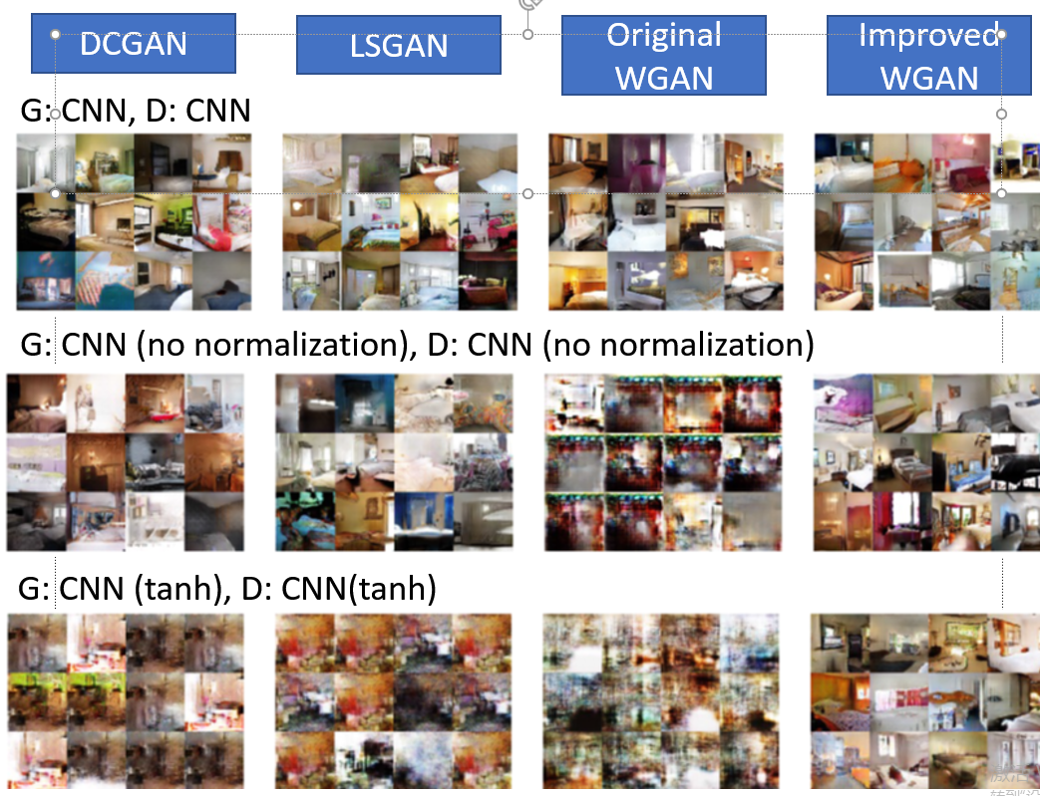
\includegraphics[width=10cm]{example/WGAN1.jpg}
	\hspace{1cm}
%	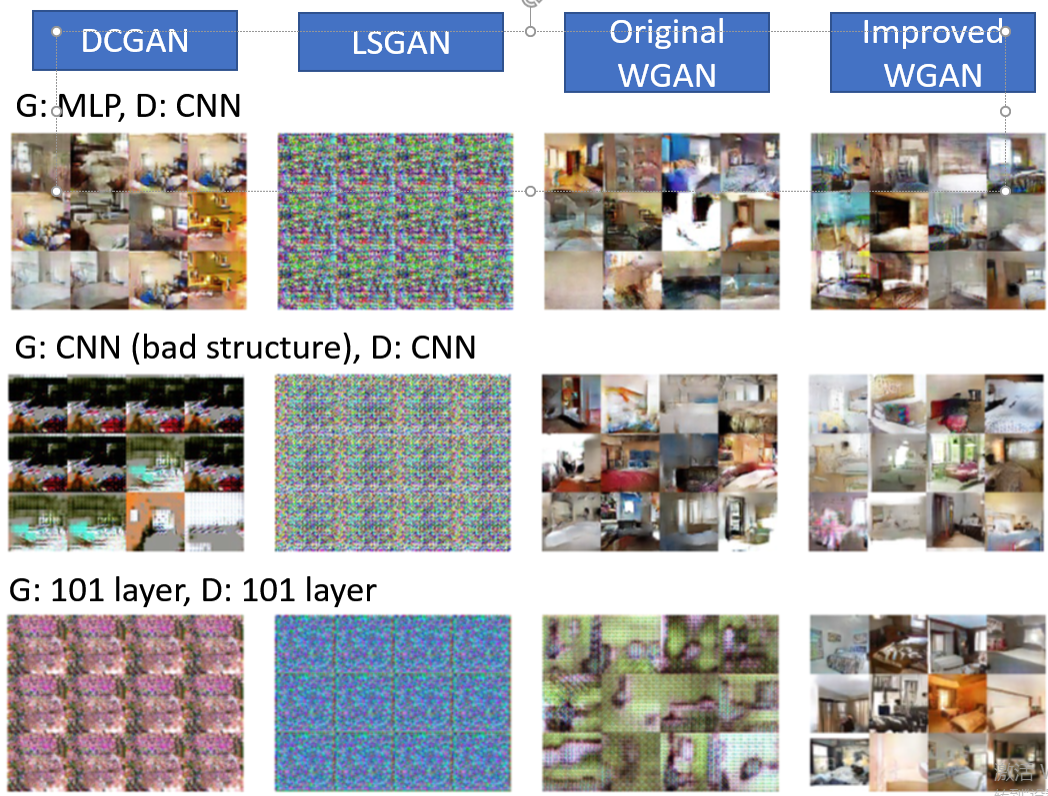
\includegraphics[width=10cm]{example/WGAN2.png}
	\bicaption[这里将出现在插图索引中]
	{GAN结构示意图}
	{Framework of GAN}
	\label{fig:GAN1}
\end{figure}

\section{改进的有监督信号的WGAN算法}
如前面内容提到的,GAN现在主要应用于图像视频领域,对于非图像类数据还没有良好的应用效果。在这一节,将详细介绍改进的WGAN算法。WGAN主要结合了自动编码机(Auto-Encoder,AE)模型学习隐向量的表征能力和WGAN提供持续梯度的优势。通过自动编码机模型引入监督信号,把原来没有监督信息的生成模型变成了利用重构误差衡量其模型好坏的方案。
\subsection{引入监督信息}
监督学习模型因为其优化的目标函数具有规则的几何形状,所以可以有效解决模型梯度消失的问题。\cite{11}。真实的样本可以通过输入隐式空间向量来重建一个性能良好的模型,这样就给生成模型提供了有监督的信号。也就是说,GAN中的生成器可以作为解码器把经过自动编码机编码后的隐向量进行解码操作,把压缩后的特征还原到原始特征空间$X$。在这种有监督的训练过程中,隐向量可以看作是低维空间$Z$中固定的先验分布。因此,先验知识由AE获得,这种方法在机器学习领域的编码工作中得到了广泛的应用。与VAE相比,AE没有额外的隐向量分布的限制。监督信号的优化目标可以描述为:  $ G(E(X))\rightarrow X $。最优的生成器可以最小化$ G(E(X))$和$X$之间的差异。在随机噪声数据的输入中加入规则信息,避免了大量的盲试过程。能够加快模型的收敛速度,提升模型的学习能力。
\subsection{变分GAN}
VAEGAN将在GAN鉴别器中学习到的特征表示作为VAE的基础。其结合方式如图\ref{figVAEGAN}所示。

\begin{figure}[!htp]
	\centering
	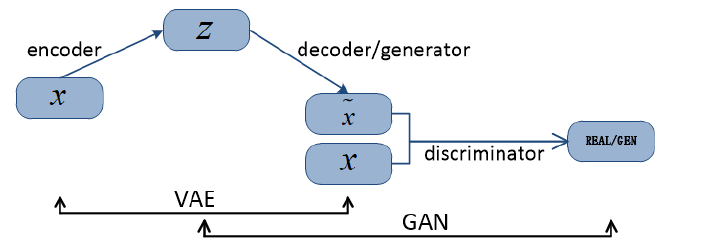
\includegraphics[width=\hsize]{example/VAEGAN.png}
	\bicaption[这里将出现在插图索引]
	{VAEGAN 结构示意图}
	{The Structure Diagram of VAEGAN}
	\label{figVAEGAN}
\end{figure}

与原始的VAE相比,VAEGANs将元素误差替换为特征误差,以更好地捕获数据分布,同时提供不变量\cite{7}。VAE的理论是概率变分界\cite{16},即:

\begin{equation}
\label{eq18}
p(x)\geq E_{q(x\mid z)}[log p (x\mid z)]- KL(q(z\mid x)\parallel P (z))
\end{equation}

然而,由于VAE的结构,VAEGAN不得不遵循这样的假设:潜在变量可以通过分解高斯分布很好地拟合,而高斯分布只有一种模式。在上述约束条件下,编码器将实际样本转化为潜在空间,使生成的潜在向量大致服从正态分布。编码器的输出是加到高斯噪声中的隐藏变量的均值和方差。VAEGAN的解码器与GAN的鉴别器具有相同的参数,即原始VAE的解码器被GAN的鉴别器所替代,这样做的好处是可以更好的了解潜在的特征。

VAEGAN使用GAN的鉴别器作为一种学习相似性度量,但没有利用GAN强大的生成能力。在数据的重构和修复上有很好的效果,但是在数据增强表现一般。VAE是基于潜伏期向量可以近似为高斯分布的假设。然而,对于单模态下不能拟合出潜在空间的GAN,这种假设是不必要的。

虽然WGAN解决了梯度消失的问题,并提供了生成样本的直接评价准则,但是没有对象能够保证遍历所有模式的样本。模态崩溃仍然是一个主要问题。发生器的输入是高斯噪声,其随机性导致训练过程不稳定,收敛缓慢\cite{17}等问题,这种现象在训练初期尤为明显。

到目前为止,所有的VAEGAN和WGAN实验都是基于CIFAR-10、LSUN睡房数据集和MNIST等图像数据,取得了显著的效果。GAN的应用领域还没有扩展到非图像的机器学习领域。

\subsection{改进的WGAN算法描述}
改进的WGAN的具体实现过程为:
除了高斯噪声,隐式特征向量也一起作为输入数据传给生成器,作为数据生成的额外附加信息,隐向量携带着数据本身的一些信息。将AE与WGAN相结合,可以在编码器中使用学习到的特征表示作为WGAN生成目标的基础。改进算法的框架如图~\ref{fig2}所示。

\begin{figure}[!htp]
	\centering
	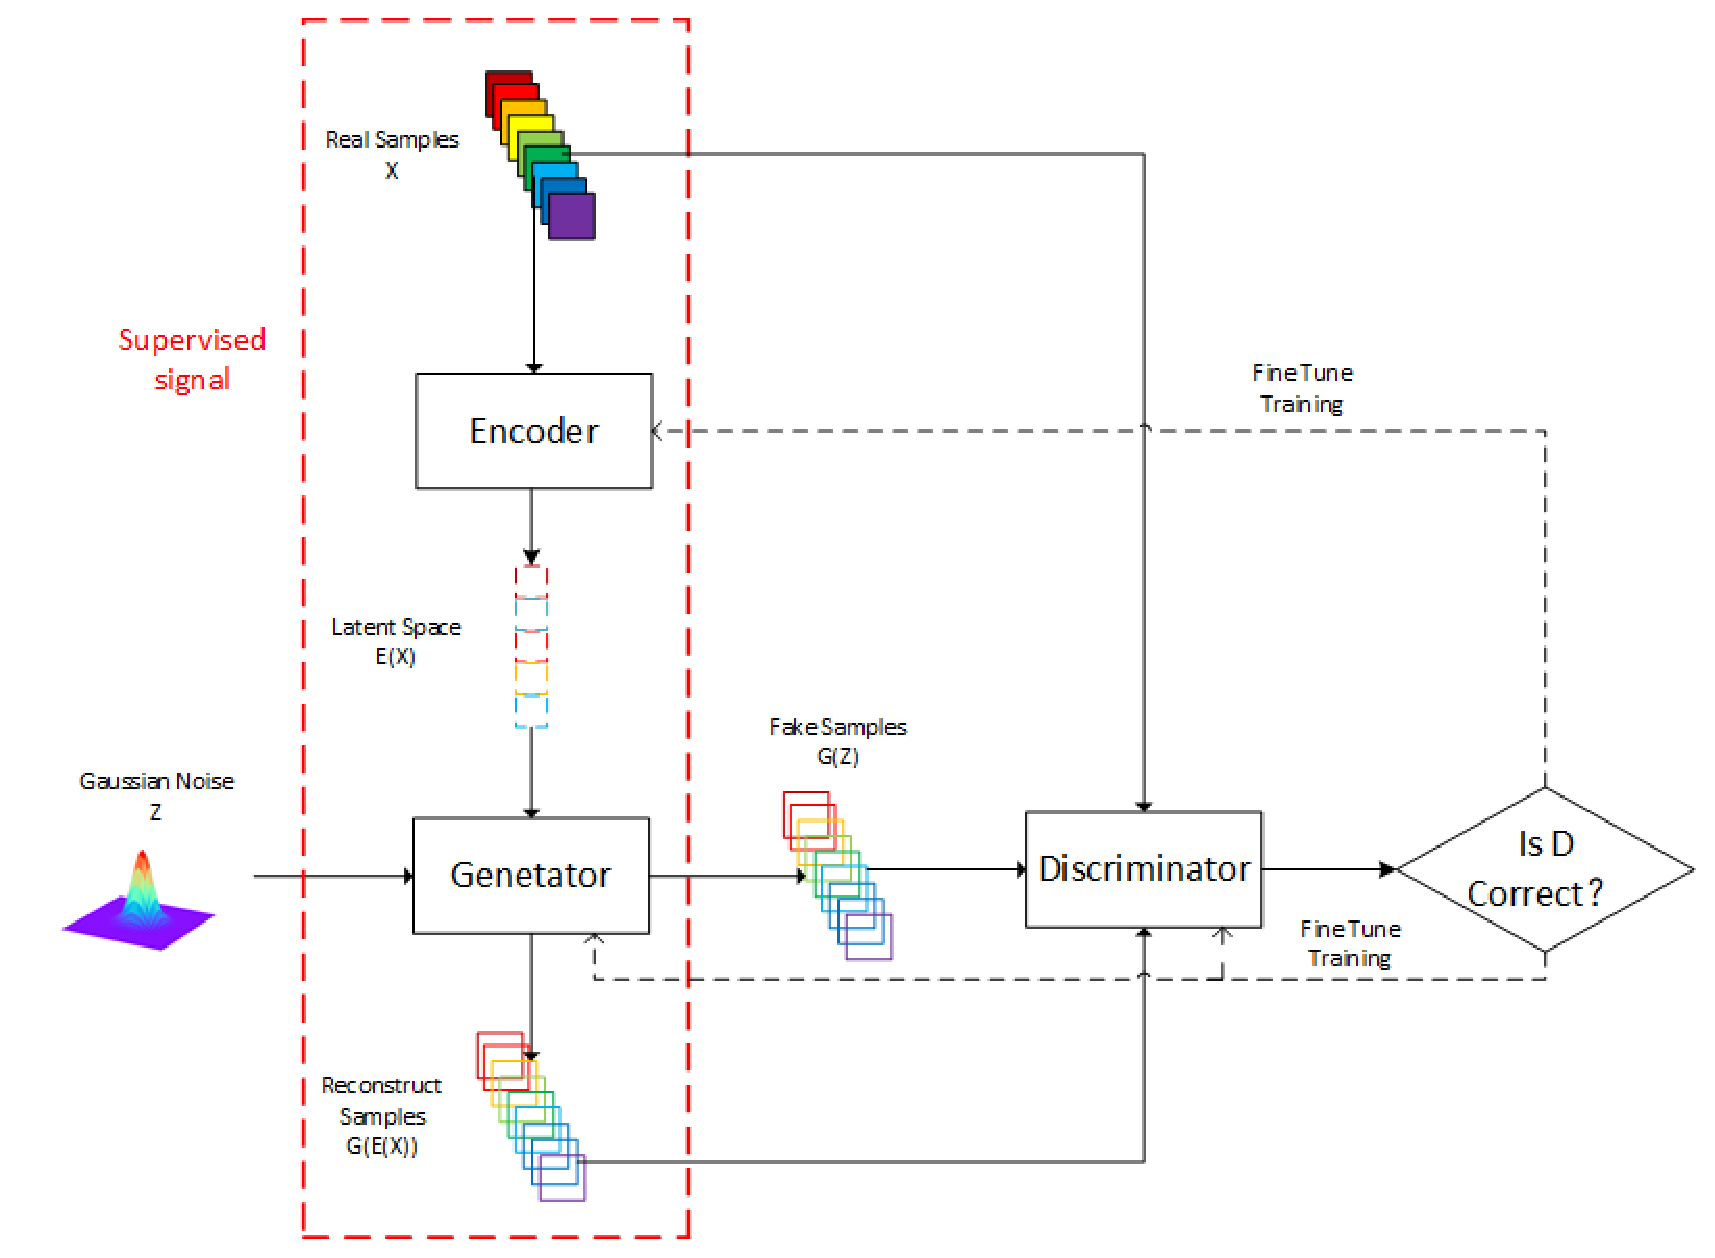
\includegraphics[width=\hsize]{example/2.eps}
	\bicaption[这里将出现在插图索引]
	{带监督信号的WGAN流程图}
	{Flowchart of WGAN with Supervised Signal}
	\label{fig2}
\end{figure}

图~\ref{fig2}中的所有样本都是一维非图像类数据集。可以看到除噪声数据外,还将自动编码机获得的隐向量数据表示形式输入到生成器中。生成器将隐藏变量转换为重构样本,优化的目标是期望重构样本尽可能接近真实样本。判别器通过最大限度地提高真样本和假样本的差异,从假样本、重构样本和真样本中获取信息。同时,生成器的目标是产生判别器无法区分的伪样本。判别器和生成器的训练过程是对抗性的。因为带监督信息的编码机能够遍历所有的原始样本,在原始数据中所有的分布都可以被模型学习到。有监督信号有助于学习到的概率密度函数能够均匀的分布在所有有原始样本的空间,从而为模态崩溃提供了有效的解决方案。这样生成的样本类型就不会过于单一。元素方向误差是在原有特征方向误差的基础上提高整体结构稳定性的一种方法。

在这里,编码器用于获取数据潜在的特征数据,通过最小化像素级别的误差 $ L ^ { 2 } $距离来提供更多信息:

\begin{equation}
\label{eq11}
T_{encoder} = D_{reconstruction}=\parallel X-G(E(X))\parallel^{2}
\end{equation}

这么做的好处是生成器可以将噪声样本$Z$和潜在样本$E(X)$分别转化为伪样本和重构样本,并从判别器那里获得较高的置信度系数。和原来的WGAN类似,这里我们仍旧使用Wasserstein距离作为统计标准来衡量两个数据分布的接近程度。这样经过引入了监督信号,新的算法优化目标函数变为:
\begin{equation}
\label{eq12}
T_{G} = -D(G(Z))-D(G(E(X)))+\parallel X-G(E(X))\parallel^{2}
\end{equation}

这里面$Z$ 是从简单的噪声分布中采样得到的数据,噪声的分布可以是均匀分布或者是高斯分布。对于判别器,$X$ 是真实的数据,因此应该能够得到较高的置信度。$G(Z)$ 和 $G(E(X))$都是假样本,应该从判别器那里得到比较低的打分值。这个过程的优化目标函数可以描述为:

\begin{equation}
\label{eq12}
T_{D} = D(X)-D(G(E(X)))-D(G(Z))
\end{equation}

整个算法的流程如下所示:

\begin{algorithm}[htpb]
	\caption{有监督信号的WGAN}% Ëã·¨±êÌâ
	\begin{algorithmic}[1]%Ò»ÐÐÒ»¸ö±êÐкÅ
		\Require ~~ \\
		对于生成器每次更新,判别器更新的次数$n_{critic}$,批训练样本大小$m$,训练迭代次数为 $K$.
		\For{$t=1$ to $K$}
		\For{$i=1$ to $n_{critic}$}
		\State 从噪声数据$Z$中采样$m$个数据:${z^{(1)},...,z^{(m)}}$
		\State 从真实数据$X$中采样$m$个数据:${x^{(1)},...,x^{(m)}}$ 
		\State 利用随机梯度上升法更新判别器网络参数:
		\begin{equation*}
		\nabla_{\theta_{d}}\frac{1}{m}\sum_{i=1}^m[D(x^{(i)})-\lambda {\rm{D(G(E(x^{(i)})))}}-D(G(z^{(i)}))]  
		\end{equation*}
		\EndFor
		\State 从噪声数据$Z$中采样$m$个数据:${z^{(1)},...,z^{(m)}}$
		\State 从真实数据$X$中采样$m$个数据:${x^{(1)},...,x^{(m)}}$
		\State 利用随机梯度下降法更新生成器网络参数:
		\begin{equation*}
		\nabla_{\theta_{d}}\frac{1}{m}\sum_{i=1}^m[-D(G(z^{(i)}))-\lambda {\rm{D(G(E(x^{(i)}))}}+\parallel x^{(i)}-G(E(x^{(i)})\parallel^{2}]
		\end{equation*}
		\State 利用随机梯度下降法更新自动编码器网络参数:
		\begin{equation*}
		\nabla_{\theta_{d}}\frac{1}{m}\sum_{i=1}^m[\parallel x^{(i)}-G(E(x^{(i)})\parallel^{2}]
		\end{equation*}
		\EndFor
	\end{algorithmic}
\end{algorithm}
\section{模型性能分析}
在本节将就改进模型的有效性和在标准数据集下不同参数中的表现进行分析,确定合理的参数方案。
\subsection{模型有效性分析}
由于数据的分布很难直观的观察到,为了可视化数据,首先生成一维概率密度分布已知的数据,从中采样得到相应的真实样本数据,把这些真实样本数据作为GAN网络的输入数据,然后绘制输出学习到的数据分布。观察生成数据和原始真实数据的吻合程度。

首先假设原始数据分布为两个高斯分布的叠加,第一个高斯分布为$\mu=4,\sigma=0.5$,第二个高斯分布为$\mu=0,\sigma=0.3$。原始数据分布形式如下:
\begin{figure}[!htp]
	\centering
	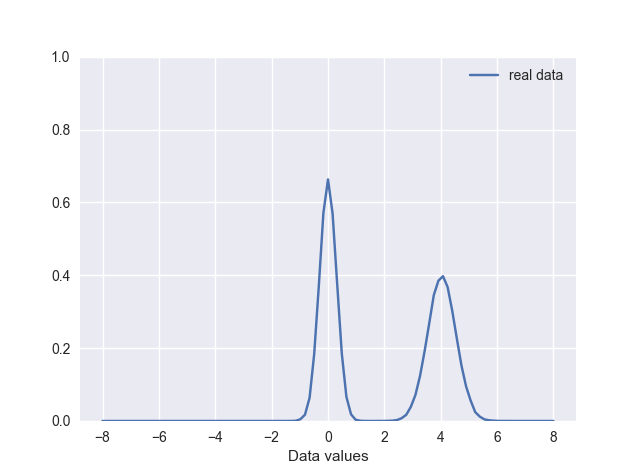
\includegraphics[width=\hsize]{example/yuanshi.png}
	\bicaption[这里将出现在插图索引]
	{原始高斯分布}
	{Flowchart of WGAN with Supervised Signal}
	\label{figyuanshi}
\end{figure}
对比WGAN,VAEGAN和改进的GAN算法,使用相同的网络结构,扩充数据量都为10000条,绘制扩充后的数据和原始数据的概率密度对比图如下:

\begin{figure}[!htp]
	\centering
	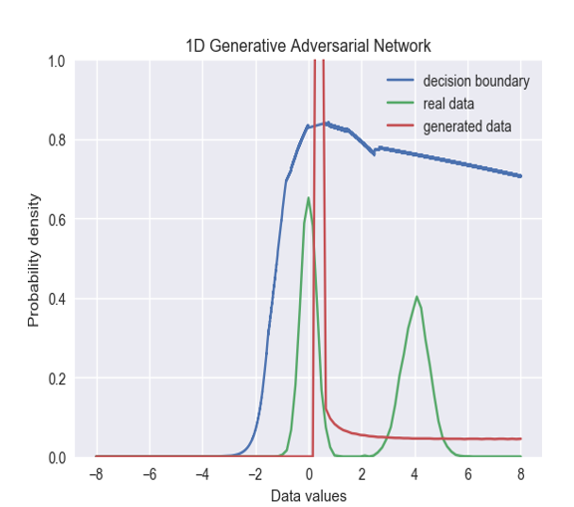
\includegraphics[width=10cm]{example/tu1.png}/
	\hspace{2cm}
	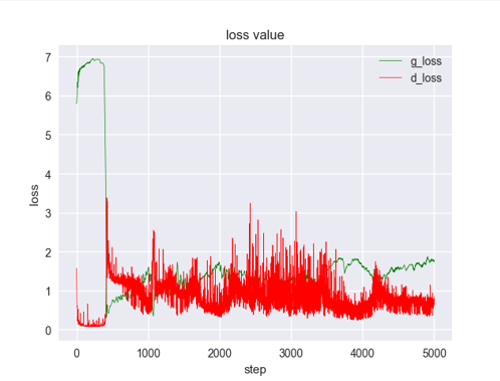
\includegraphics[width=10cm]{example/loss1.png}
	\bicaption[这里将出现在插图索引中]
	{WGAN 实验效果图}
	{Framework of GAN}
	\label{fig:al1}
\end{figure}
\begin{figure}[!htp]
	\centering
	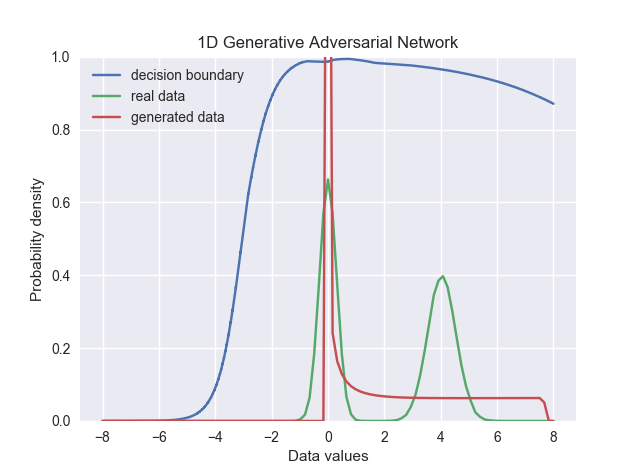
\includegraphics[width=10cm]{example/tu2.png}/
	\hspace{2cm}
	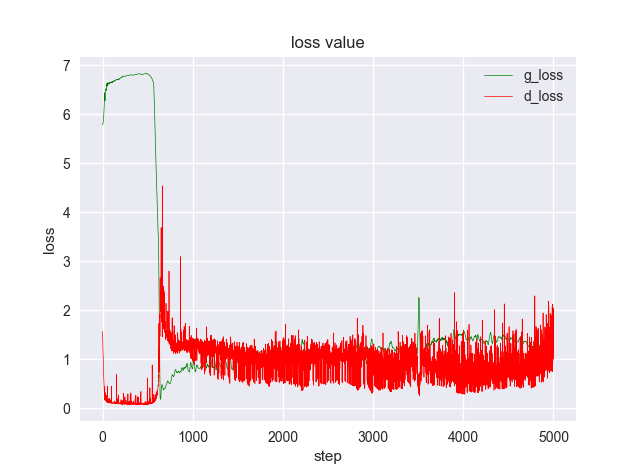
\includegraphics[width=10cm]{example/loss2.png}
	\bicaption[这里将出现在插图索引中]
	{VAEGAN实验效果图}
	{Framework of GAN}
	\label{fig:al2}
\end{figure}
\begin{figure}[!htp]
	\centering
	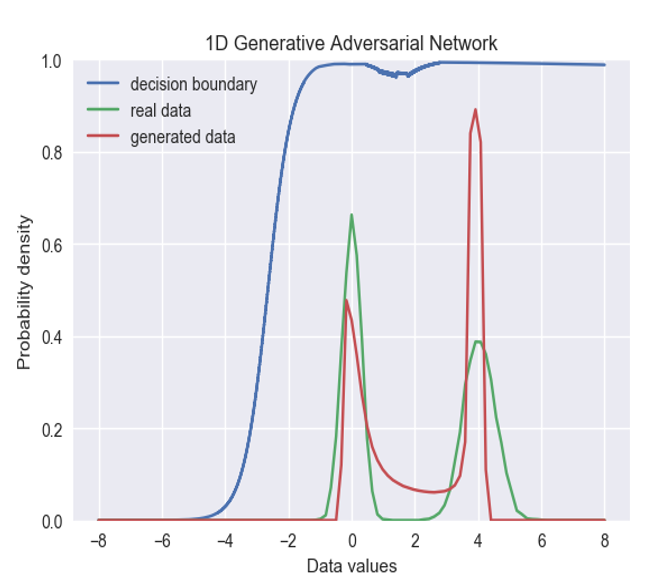
\includegraphics[width=10cm]{example/tu3.png}/
	\hspace{2cm}
	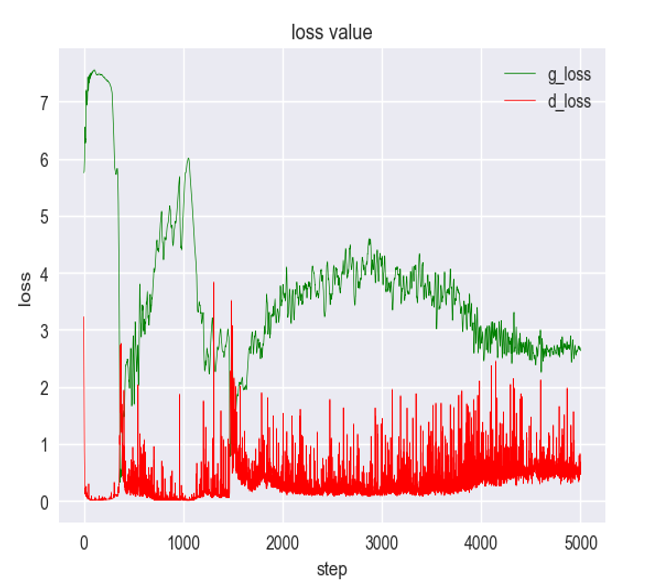
\includegraphics[width=10cm]{example/loss3.png}
	\bicaption[这里将出现在插图索引中]
	{改进WGAN实验效果图}
	{Framework of GAN}
	\label{fig:al3}
\end{figure}
可以看出,对于GAN算法,生成的数据只能学习到单高斯峰,而且生成的数据并不能准确描述$\mu=0,\sigma=0.3$的分布。判别器判别曲线还可能够判别出真假数据。从损失函数曲线上分析,两个网络始终没有达到相对稳定的状态。对于WGAN算法,仍然不能很好描述所有数据分布,但是由于引入了Wasserstein距离,损失函数曲线相比于GAN更加稳定,生成数据能相对准确的描述其中一个高斯分布,对于改进的WGAN算法,生成器已经能学到两个高斯分布,并且效果比前两种算法有所改善。对于损失函数生成器的损失函数大体呈下降趋势。通过对一维数据进行可视化,可以看出改进的算法在一定程度上改善了学习数据分布不全面,损失函数下降困难的问题。
\subsection{参数分析}
本节将结合标准数据集中联合循环发电厂(Combined Cycle Power Plant, CCPP)数据集讨论不同$\lambda$参数对实验结果带来的影响。该数据集包含了一个联合循环电厂在6年(2006-2011)的全负荷运行中收集到的9568个数据点。特征包括小时平均环境变量温度(T)、环境压力(AP)、相对湿度(RH)和排气真空(V),用于预测工厂的净小时电能输出(EP)。
数据集的描述如下:
\begin{table}[!hpb]
	\centering
	\caption{CCPP数据集描述}
	\label{tabccpp}
	\begin{tabular}{llll} \toprule
		属性名   & 描述 & 数据类型&数据范围  \\  \midrule
		Temperature&温度&浮点型(连续性)&$1.81^\circ C$, $37.11^\circ C$\\
		Ambient Pressure&环境压力&浮点型(连续性)&992.89, 1033.30 milibar\\
		Relative Humidity&相对湿度&浮点型(连续性)& 25.56$\%$, 100.16$\%$ \\
		Exhaust Vacuum&排气真空度&浮点型(连续性)&25.36, 81.56 cm Hg\\
		Hourly electrical energy output&每小时电能输出&浮点型(连续性)&420.26, 495.76 MW\\ \bottomrule
	\end{tabular}
\end{table}

原始数据量为9568个,用改进的WGAN算法扩充100000个,加入原始数据中观察数据扩充效果。设定生成数据量的大小都为选用的衡量指标是均方误差,通过设置不同$lambda$参数,平衡损失函数中数据生成和数据解码之间的关系。

为了评价新算法生成的样本质量,把所有数据归一化后,采用SVR模型进行回归,这里SVR使用径向基核函数。更多的拟合先验分布的伪样本可以改善回归结果。均值平方误差(Mean squared error, MSE)是一种反映SVR回归准确率的评价标准,用于间接检验数据增强实验的有效性。MSE的定义可以用公式\ref{eq14}表示:

\begin{equation}
\label{eq14}
MSE=\frac{\sum \limits_{i=1}^m (y^{i}-\bar{y})^{2}}{m}
\end{equation}

在这里 $y^{i}$ 是SVR预测的标签值,$\bar{y}$ 是原始数据的真实标签,测试数据集中有$m$样本,MSE值越小,误差越小,得到的生成样本越好。

图\ref{figCCPP}为CCPP数据集在不同$\lambda$参数下面的性能表现。
\begin{figure}[!htp]
	\centering
	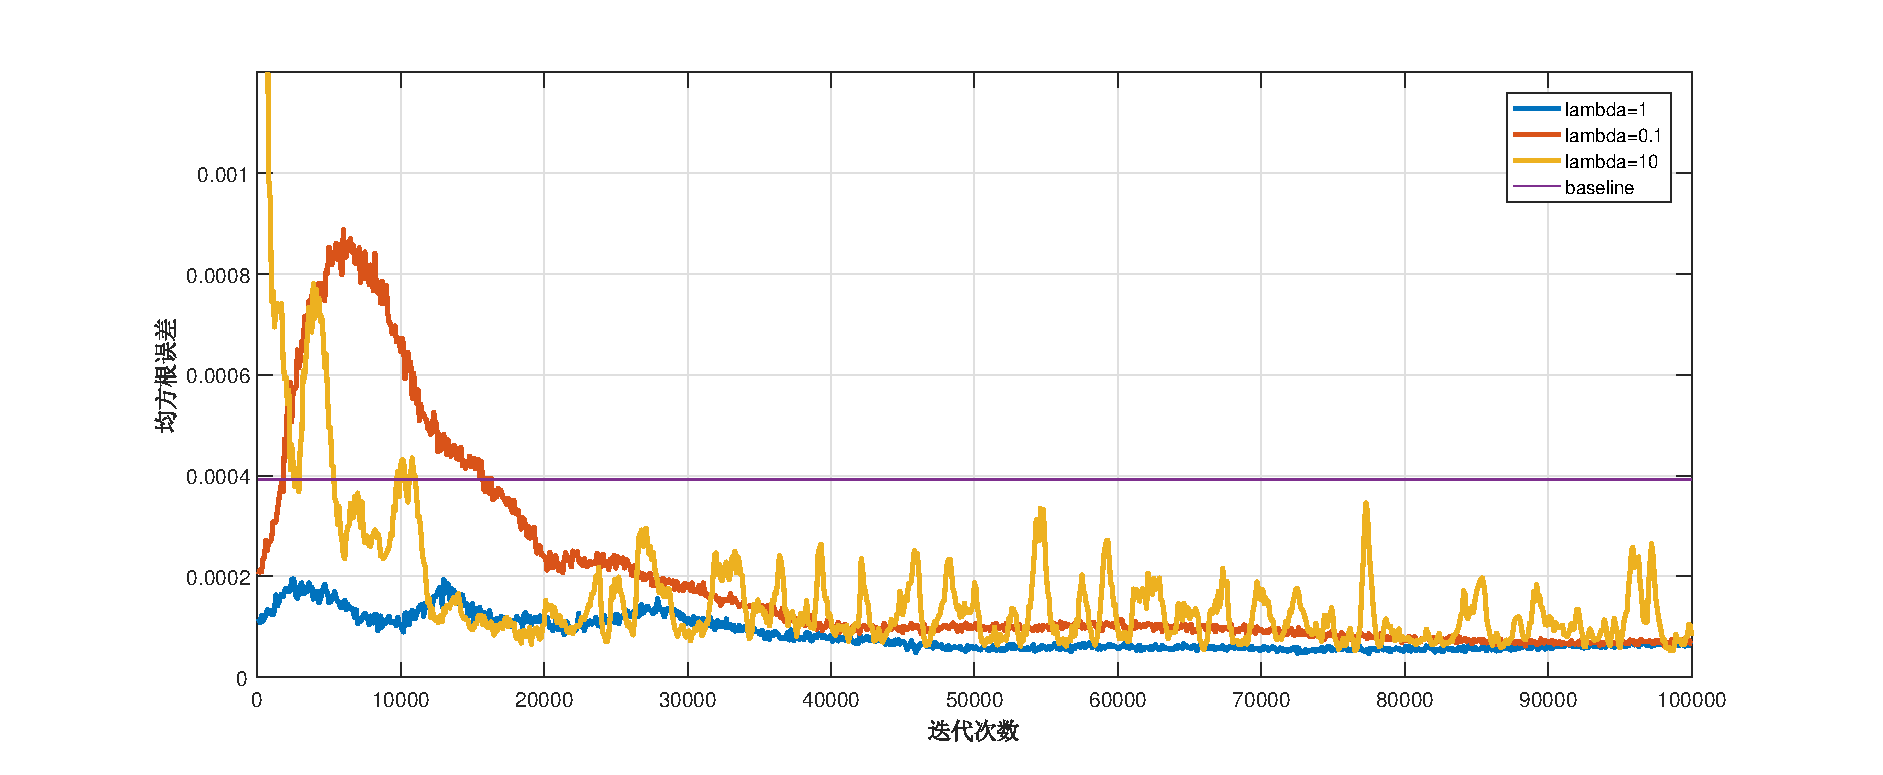
\includegraphics[width=\hsize]{example/CCPP.eps}
	\bicaption[这里将出现在插图索引]
	{CCPP数据实验结果}
	{Flowchart of WGAN with Supervised Signal}
	\label{figCCPP}
\end{figure}

可以看出,当$\lambda=10$时,改进的模型AE解码作用占比重相对较大,整个算法回归效果在前期并不理想,后期也存在严重的抖动问题。当$\lambda=0.1$,AE模型占比相对较小,无法知道GAN生成数据的方向,前期生成网络随机生成大量假样本,干扰了数据的质量,$\lambda=1$相对合理的平衡了生成模型和AE模型的权重,在网络的初始阶段曲线相对稳定,生成数据的质量相对较高,到后期随着迭代次数增加,MSE呈缓慢下降趋势。可以看出在迭代次数80000次后,曲线呈上升趋势,分析这是由于深度学习网络过拟合造成的,解决方案就是采用监控损失函数曲线,当发现loss呈上升趋势进行早停处理。


\section{实验结果及分析}
本节将给出实际的仿真结果和相应的结论。现有的GAN训练实验大多基于图像数据或视频数据。本文将改进后的新算法应用于一维数据的扩展。在这一部分,首先介绍评价数据扩充的标准,为了验证改进算法的可行性,分别对所测电子设备参数和5个指数股票序列数据集进行了实验,通过对比改进WGAN和传统算法进行数据扩充的结果进行分析。


在这里 $y^{i}$ 是SVR预测的标签值,$\bar{y}$ 是原始数据的真实标签,测试数据集中有$m$样本,MSE值越小,误差越小,得到的生成样本越好。

\subsection{电子设备参数实验}

本节数据集来自洛阳电子对抗基地。特征值的个数为10,输出响应变量为二维。另外,数据样本有72个,其中选择60个数据样本进行训练,选择12个样本进行测试。将改进算法应用于电子设备参数,验证了算法的稳定性。为了进行对照实验,也使用了VAEGAN和WGAN。对于编码器、解码器、生成器和判别器,所有对比模型都具有相同的架构。模型使用RMSProp优化算法进行训练,学习率为0.0003,批大小为24。表\ref{tab3}中列出了网络架构。

\begin{table}[hpb]
	\centering
	\caption{网络结构参数}
	\label{tab3}
	\begin{tabular}{lll} \toprule
		编码器   & 生成器 & 判别器  \\  \midrule
		12 fully-connected, ReLU &12 fully-connected, ReLU&12 fully-connected, ReLU\\
		24 fully-connected, ReLU&24 fully-connected, ReLU&24 fully-connected, ReLU\\
		24 fully-connected, None&24 fully-connected, ReLU&24 fully-connected, ReLU\\
		&12 fully-connected, None&1 fully-connected, None\\ \bottomrule
	\end{tabular}
\end{table}

训练迭代次数相同:选择60000次,生成的数据样本个数为25000个。通过生成的数据对测试数据进行回归,MSE值在迭代过程中发生变化,如图~\ref{fig3}所示。

\begin{figure}[htpb]
	\centering
	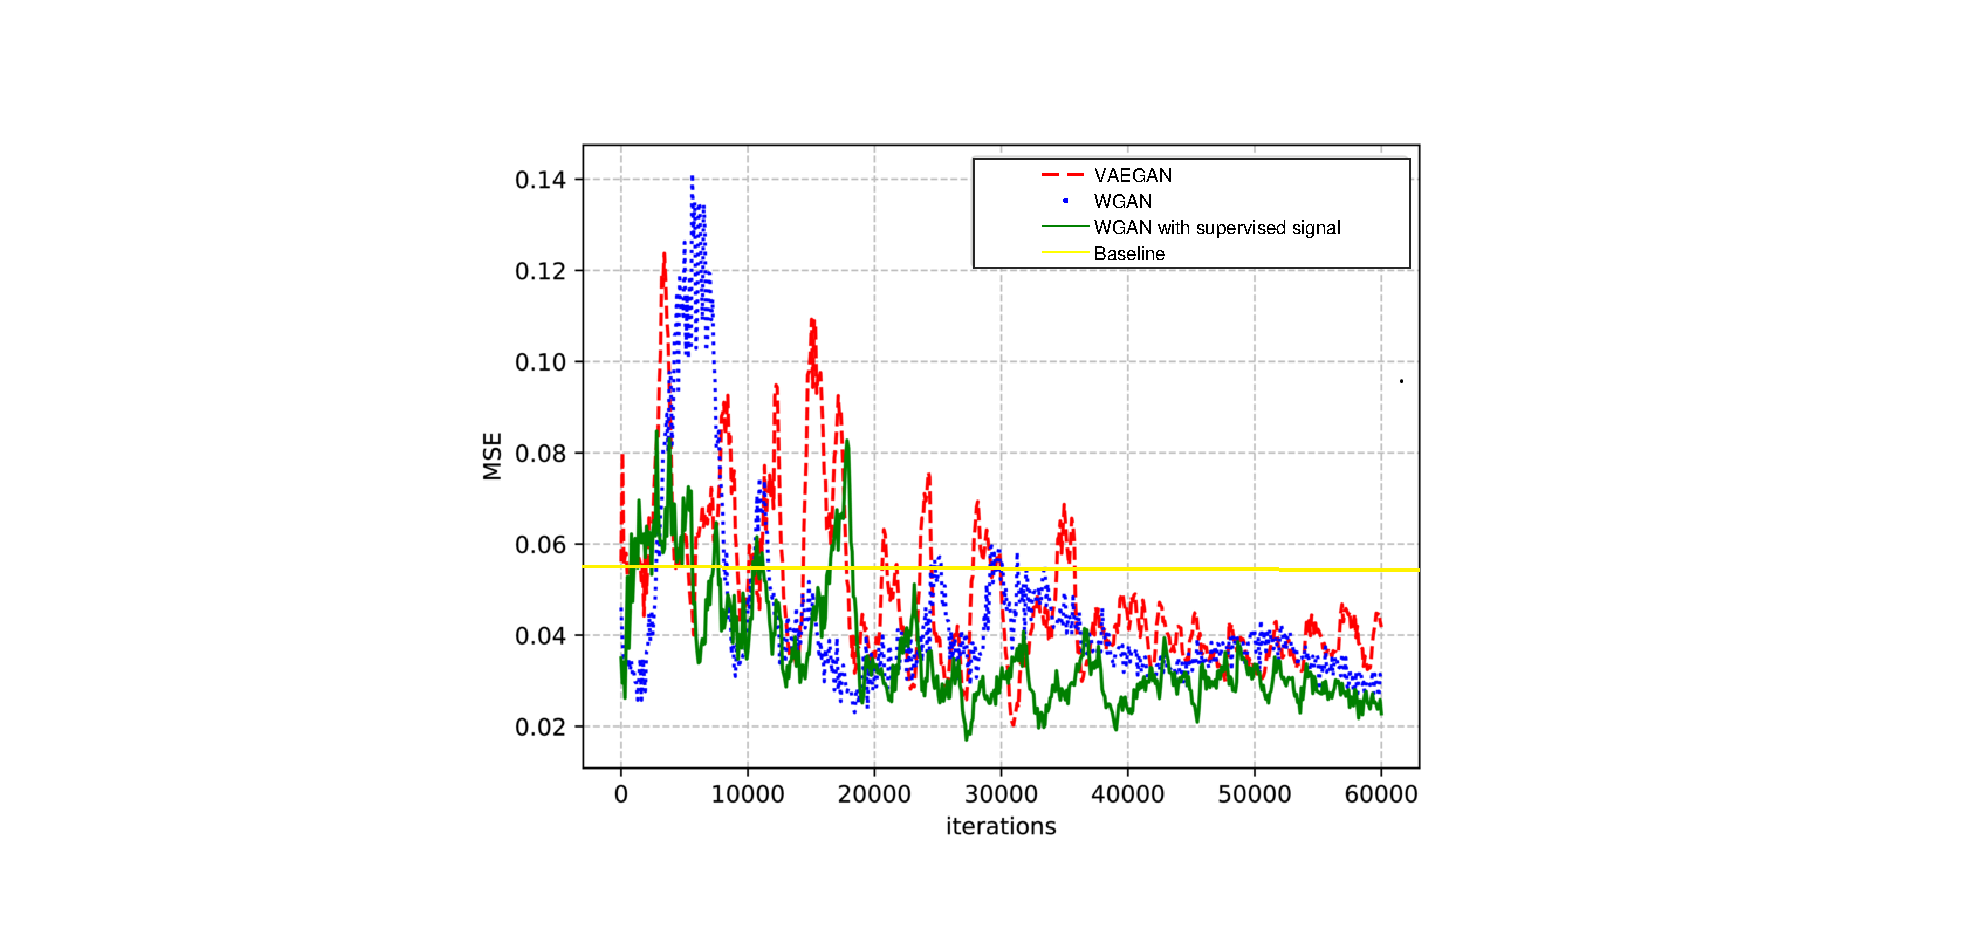
\includegraphics[width=\hsize]{example/GANsuanfaduibi.eps}
	\bicaption[这里将出现在插图索引]
	{不同模型生成数据进行回归MSE曲线图}
	{Mean squared error of different algorithms}
	\label{fig3}
\end{figure}

如图~\ref{fig3}所示,改进算法与VAEGAN和WGAN相比收敛速度更快,回归效果更好,反映了改进算法生成的样本更接近原始数据分布。在30000次迭代中,改进算法达到了稳定。由于有监督信号具有固定的先验分布,改进算法在训练初期的MSE明显低于其他算法。

\subsection{对于股票数据的回归}

为了消除实验的偶然性,我们分别对5个股票指数序列数据集进行了算法检验。与第4.1款设计的架构相同。表~\ref{tab1}给出了五种主要的股票价格指数,并使用了代码名。

\begin{table}[hpb]
	\centering
	\caption{股票数据详情}
	\label{tab1}
	\begin{tabular}{lll} \toprule
		股票价格指数   & 代码名称 &  数据区间  \\  \midrule
		All ordinaries   & AORD&  01/01/2016 to 01/09/2017 \\
		Dow Jones Industrial Average   & DJI&01/01/2016 to 01/09/2017\\
		Hang Seng Index   & HSI&   01/01/2016 to 01/09/2017\\
		KOSPI   & KS11& 01/01/2016 to 01/09/2017\\
		Nikkei Stock Average   &NK&   01/01/2016 to 01/09/2017\\
		\bottomrule
	\end{tabular}
\end{table}

这些数据来自雅虎财经网站\footnote{\url{https://finance.yahoo.com/}}。原始数据包括每天的开盘价、收盘价、最高价、最低价和成交量。选择增加收盘价。采用特征向量法\cite{18},利用最新的价格计算特征来处理序列数据。根据坐标延迟法,输入向量的维数为$m$,延迟时间为$d$,输入向量为$RDP_{1,d},…,RDP_ {m - 1 d}, EMA_{15}$和输出向量$RDP_ {d} $:

\begin{equation}
\label{eq16}
RDP_{i,d} = \frac{p(j)-p(j-i*d)}{p(j-i*d)}*100
\end{equation}


\begin{equation}
\label{eq17}
EMA_{15}  = p(j)-\bar{EMA_{15}(j)}
\end{equation}

\begin{equation}
\label{eq18}
RDP_{d} = \frac{\bar{p(j+d)}-\bar{p(j)}}{\bar{p(j)}}*100
\end{equation}


其中 $p(j)$ 是在时间点 $j$的价格。本文选择延迟时间$d=5$,输入向量维度$m=5$。分割前$80\% $的数据是训练数据,后$20\% $的数据是测试数据。分别利用VAEGAN、WGAN和我们算法对转换后的数据进行实验。回归结果如表\ref{tab2}:

\begin{table}[hpb]
	\centering
	\caption{股票数据回归结果}
	\label{tab2}
	\begin{tabular}{lllll} \toprule
		股票名称 & GAN &  VAEGAN & WGAN &Ours  \\ 
		\midrule
		AORD&0.01184 & 0.00667 & 0.00764 &\textbf{0.00622}   \\
		DJI &0.00816&0.00737&0.00769&\textbf{0.00643}  \\
		HSI&0.01762&0.01585&0.01612&\textbf{0.01409}  \\
		KS11&0.02655&0.02465&0.02621&\textbf{0.02413}\\
		NK & 0.07398& 0.03836& 0.04298&\textbf{0.03445} \\
		\bottomrule
	\end{tabular}
\end{table}

如表\ref{tab2}所示,利用带监督信号的WGAN实现非图像数据的增强是具有可行性的,对比于其他模型,表现出了更好的回归效果。本文提出的算法增加了有监督信号,该信号可以通过输入样本的潜在特征来约束生成器遍历所有真实样本。
改进后的算法有两个优点:
\begin{enumerate}
	\item 用自动编码机对数据编码的过程可以获得额外的学习知识,这使得生成器产生的伪样本很难被鉴别器识别。在有监督信号的情况下,生成的数据分布与之前的真实数据分布具有一对一的匹配关系,其对应关系保证生成的网络覆盖了真实数据的所有模式。
	\item 监督信号增强了WGAN输入的先验信息,避免了训练初期由于大量初始化参数而产生的随机样本,加快了训练过程,提升了生成样本的质量。
\end{enumerate}

\section{本章小结}

本章主要介绍了用强化学习模型进行数据增强的生成式对抗网络。在本章的第一部分介绍了GAN的背景意义,作为生成式模型的一种,GAN相对于传统的其他模型表现出了优良的性能。第二部分介绍了GAN的基本组成成为及算法的实现过程。GAN的生成器和判别器分别对应于强化学习Actor-Critic框架的Actor和Critic。在本章的第三部分介绍了GAN的优化算法WGAN,引入了Wasserstein距离的概念,并解释了为什么用Wasserstein来衡量数据分布的距离要优于其他度量参数。在本章的第四部分创新性的提出了引入监督信息的WGAN算法应用于非图像类数据的数据增强,其关键思想是在WGAN与编码器相结合时,通过输入样本的潜在特征来构造真实的样本。在描述改进算法的网络结构和优化的损失函数之后,文中给出了算法具体的实现过程。接着在文章的第五部分,针对改进的算法分别对实测的电子设备参数数据,和股票数据的回归问题上进行了实验,从理论上和实验上验证了新算法的可行性。

在训练初期,随着对原始参数的大量尝试的减少,改进的引入监督信息的WGAN收敛速度比其他两种算法都要快。新算法生成的数据更接近真实数据的分布。
%# -*- coding: utf-8-unix -*-
% !TEX program = xelatex
% !TEX root = ../thesis.tex
% !TEX encoding = UTF-8 Unicode
%%==================================================
%% chapter01.tex for SJTU Master Thesis
%%第四章
%%==================================================
\chapter{基于深度强化学习的棋盘类博弈策略}
计算机博弈经常被认为是人工智能领域面临的挑战之一,在现实应用中由博弈模型发展出的算法在很多领域都有成功的应用。在本章,将详细介绍博弈理论的基本知识,基于深度强化学习模型对单智能体一对一博弈策略的研究。
\section{引言}
作为人工智能的重要载体,机器博弈已经渗透到人类社会生活的各个领域:如利用博弈理论做用户数据分析\cite{吴诚2017基于博弈论的大用户直购电双边决策研究},网络防御系统的搭建\cite{许晓燕2018基于博弈模型的网络防御},电力需求侧分析\cite{刘晓峰2018博弈论在电力需求侧的应用研究综述},房产土地竞标\cite{朱传军2011基于模糊测度与模糊积分的房地产评估方法与应用},等等。

常见的博弈模型分为完备信息的博弈模型,和非完备信息的博弈模型。完备信息是指博弈双方都已知当前的局面状态并能感知历史信息,非完备信息博弈是指博弈双方无法感知状态信息或者只能感知部分状态信息进行相互博弈。根据博弈双方最后取胜目标又可以分为零和博弈和非零和博弈。零和博弈是指博弈的双方最后获取的总奖励和为零,当一方获胜的同时必然会导致另一方的失败。零和博弈是一种非合作式的博弈模型,与之相对的是非零和博弈,即博弈的双方奖励不会因为对手奖励增加而变少。根据玩家采取动作的时效性可以分为范式博弈(Form Game)和扩展式博弈(Extensive Form Game),范式博弈是指玩家双发同时做出动作,或即使有动作有先后顺序在本回合结束之前也看不到对方当前的动作,扩展式博弈是指玩家双方交替轮流进行动作,后手玩家能够感知先手玩家所做的动作。在这里,我们主要讨论完备信息下的两人零和扩展式博弈模型起到抛砖引玉的作用。典型的完备信息零和棋盘类博弈模型有德州扑克,象棋,五子棋,围棋,等等。Alpha Go的问世更是将深度强化学习在零和博弈模型的应用推到了巅峰,Alpha Go 的算法是由蒙特卡洛搜索树,深度学习网络,强化学习Actor-Critic框架组合而成,下面将详细介绍算法的基本技术背景,整个算法框架的组成,本文结合实际应用进行的改进以及实验仿真结果。
\section{AlphaGo和AlphaZero技术背景}
围棋博弈面临的最大挑战就是其庞大的搜索空间和特征平面难以完全建立。传统的下围棋的方法有利用完全遍历的蒙特卡洛树搜索的方法和利用监督学习训练,模型的方法。然而对于一些状态空间过于庞大的系统来说,完全遍历所有可能是难以实现的,大量人工棋谱获取数据成本很高,监督信号是最后一步的胜负,中间的过程很难被监督模型学习到。对于这种具有时间延迟的监督信号,研究者开始把方案转换到了强化学习上。Alpha go 一诞生就来势汹汹:自2016年1月由谷歌DeepMind团队提出Alpha Go 成果以来,2016年3月与世界围棋冠军李世石的对弈中以4:1取得胜利,2016年,该算法在中国棋类网站注册账号和数十位中日韩围棋高手对决连续60局无一败局,接着在2017年5月的中国乌镇举办的围棋峰会上,与世界第一围棋冠军柯洁对战,以3:0获胜,等级高于世界最高水平。其成功的背后离不开以下几个基本算法的应用:基于监督学习网络的预训练。蒙特卡洛搜索树的价值评估网络训练,基于深度学习强大的拟合能力,以及基于强化学习框架的self-play形式的数据扩充。
\subsection{蒙特卡洛树}
双人零和博弈过程可以用简单描述为对于互为对手的黑方和白方,他们的奖励分别为$R^1$和$R^2$,$R^1+R^2=0$ ,当黑方获胜时黑方的奖励最大化为$R^*$,白方的奖励最小化为$-R^*$。结合强化学习思想,双方都希望自己得到的奖励最大化,这里面奖励即为最后的结果,如式\ref{eq:minmax}:
\begin{equation}
\label{eq:minmax}
{v_*}(s) = \mathop {\max }\limits_{{\pi ^1}} \mathop {\min }\limits_{{\pi ^2}} {v_\pi }(s)
\end{equation}
这里面,${v_\pi }(s) = {E_\pi }[{G_t}|{S_t} = s]$
基于完全信息的博弈问题都可以通过建立树模型来模拟对弈过程。对于棋类游戏所有对战的过程都可以用一颗树完整的表示出来。树的根节点代表输入的状态,叶节点返回最终的结果。对于简单的问题,尤其是双人对战的零和博弈问题,可以用博弈树来描述整个过程,如图\ref{fig:tree}
\begin{figure}[!htp]
	\centering
	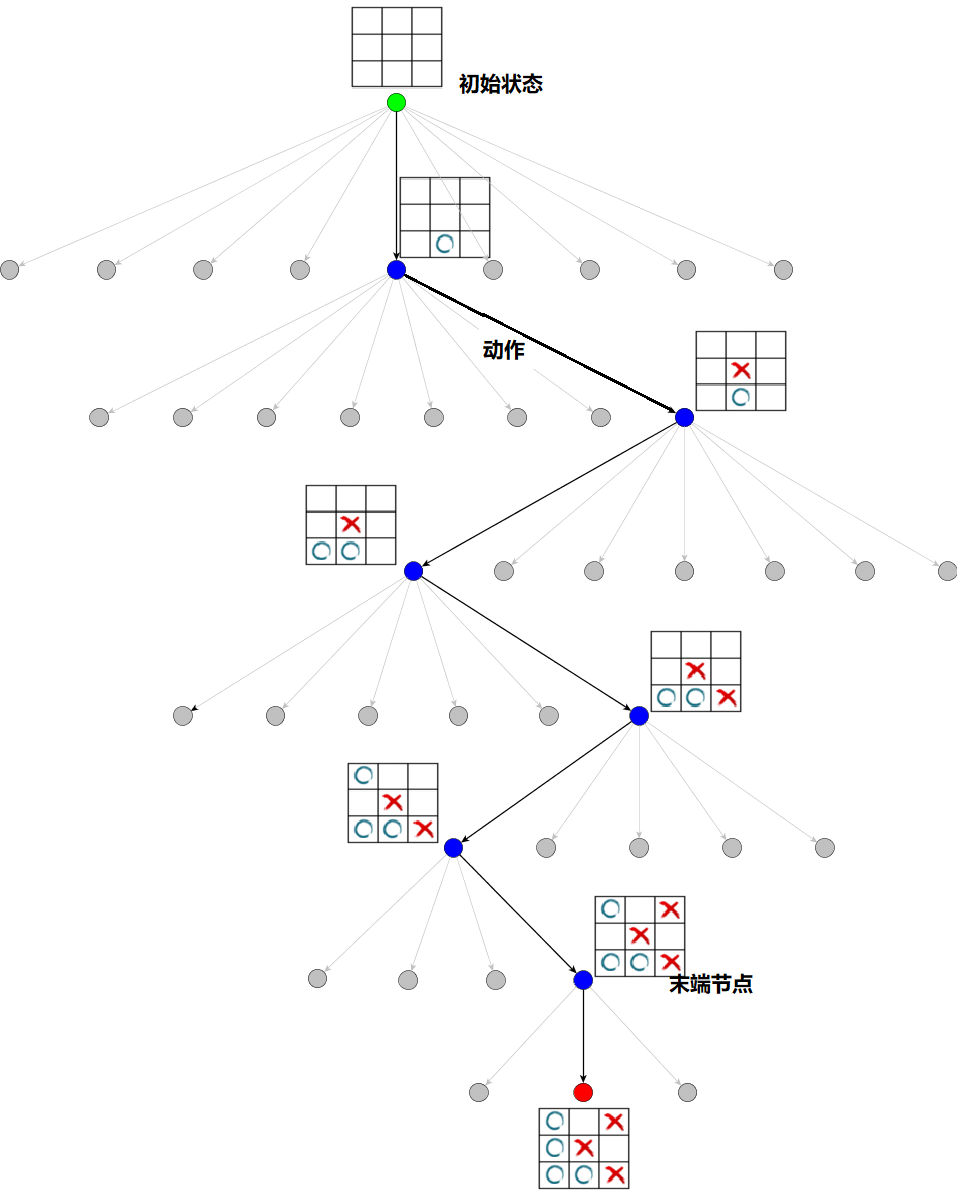
\includegraphics[width=\hsize]{example/tree.png}
	\bicaption[这里将出现在插图索引]
	{博弈树示意图}
	{The Diagrammatic Drawing of Minmax Search Tree}
	\label{tree}
\end{figure}

在博弈树中根节点代表了起始状态信息,从一个节点到其子节点的过程称为动作,节点的子节点数称为分支因子,博弈树的末端节点是博弈无法继续进行的节点,携带了游戏结束的奖励信息。博弈树是一种递归的数据结构,在每次进行一次行动后,根节点的子节点又作为下一状态信息的根节点进行进一步搜索工作。对于选择动作的方案最简单的想法就是建立一颗极小极大搜索树,其示意图如下:

\begin{figure}[!htp]
	\centering
	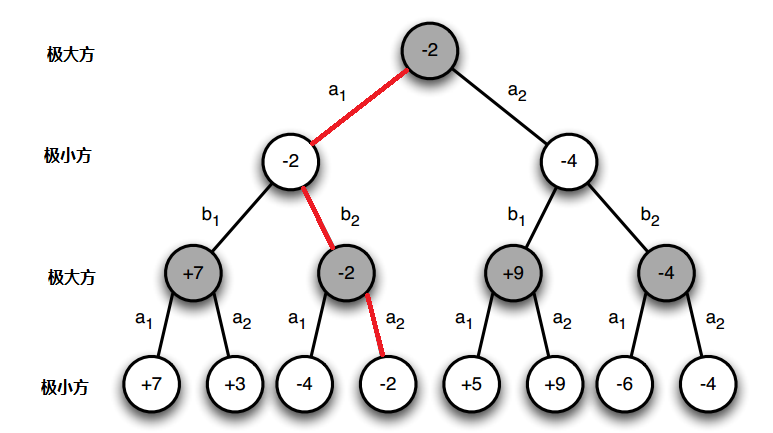
\includegraphics[width=\hsize]{example/minmax.png}
	\bicaption[这里将出现在插图索引]
	{极小极大搜索树}
	{The Diagrammatic Drawing of Minmax Search Tree}
	\label{极小极大搜索树}
\end{figure}
极小极大树提出的核心是在损失尽量小的前提下增加本方的收益,对于示意图来说,在第一步黑方是极大方,在动作选择的过程中会选择尽可能大的收益-2,对于白方来说是极小方,在第二层动作选择时会选择第二层为-2 的子节点-2,图中红色的线代表当前状态的搜索路径。这样一直循环进行选择知道游戏结束,就可以知道当前棋局下所有动作的好坏,越接近最后一步奖励的动作越被鼓励选择。但是对于搜索空间比较大的情况,遍历所有的可能是不现实的,这就需要建立更加高效的搜索树。考虑到深度网络有强大的拟合能力,可以用神经网络拟合最后的输出结果代替真实结果$v(s,w) \approx {v_*}(s)$,这样能提高搜索树的效率。此外由于会存在大量低质量的子树分支,如何在优良分支进行更多扩展,砍掉不需要的子树分支也是另一个难点。
为了解决搜索树过于庞大的问题,蒙特卡洛树应运而生,蒙特卡洛树的思想是从当前给定状态开始,随机采样后续棋局模拟,得到模拟结果,经过多次随机采样将结果的平均值返回该节点作为评估成功率的信息。一般来说节点的数据结构包括以下三个部分${Q,N,W}$,其中$Q(v)$ 为经过该节点s所获得的总评分,N为该节点及其子节点被访问的次数,W为总的奖励收益。
一个完整的蒙特卡洛树包括四个步骤如图\ref{fig:treesearch}:

\begin{figure}[!htp]
	\centering
	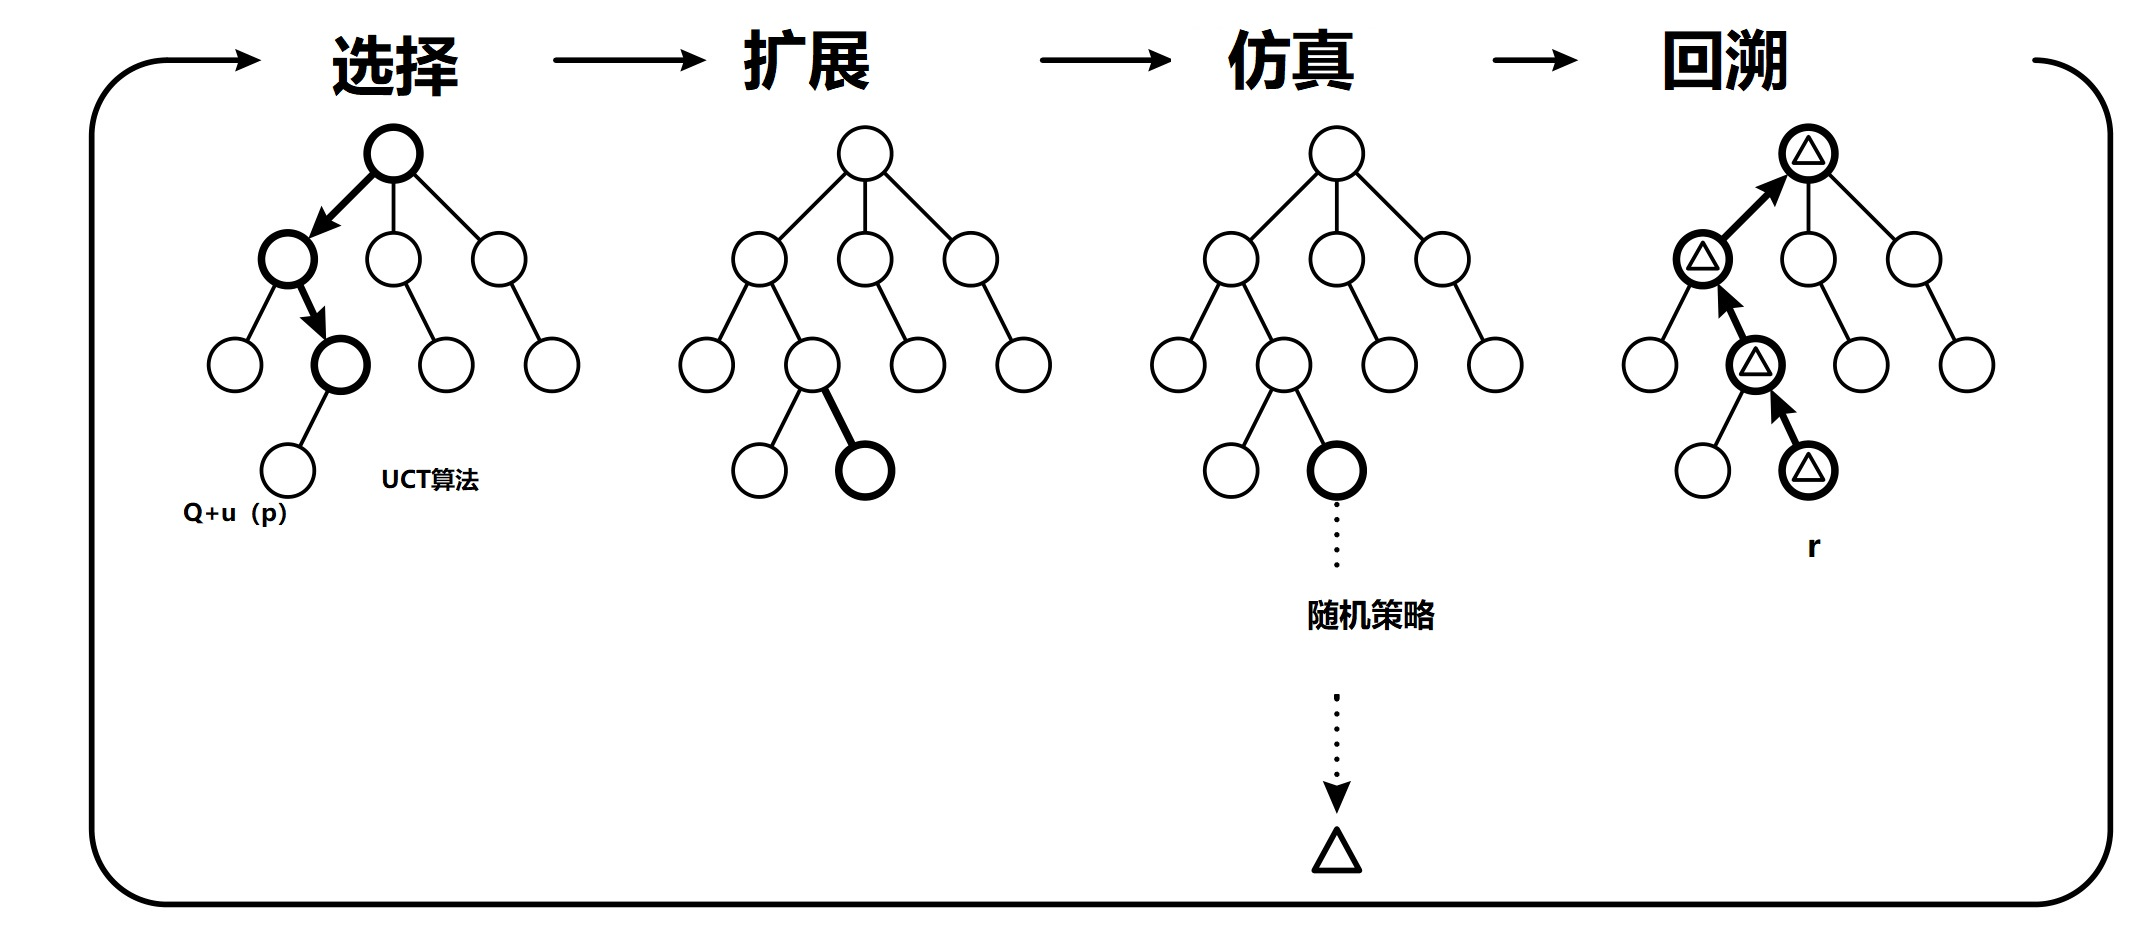
\includegraphics[width=\hsize]{example/treesearch.jpg}
	\bicaption[这里将出现在插图索引]
	{搜索树搜索示意图}
	{The Diagrammatic Drawing of Minmax Search Tree}
	\label{搜索树搜索示意图}
\end{figure}
\begin{enumerate}
	\item 选择(Selection):对于已经建立好的搜索树从根节点向下扩展到子节点选择路径的方案。
	\item 扩展(Expansion):对于没有建立好的树节点部分,在抵达叶节点其分支结构不是终止的叶子节点,在这个叶节点下建立新的叶节点。
	\item 模拟(Simulation):在上一步新建立的叶节点开始,为了评估其选择动作的好坏,随机的进行一系列动作直到结束,建立结果${\rm{R = }}\left\{ {\begin{array}{*{20}{c}}
		{{\rm{1,win}}}\\
		{{\rm{ - 1,loss}}}
		\end{array}} \right.$
	\item 回溯(Backpropagation):利用最终奖励值,把结果返回给从$C$到根节点的连边信息:$Q \leftarrow \frac{W}{N},W \leftarrow W + R,N \leftarrow N + 1$
\end{enumerate}

下面分别介绍这几个步骤的具体实现过程

在选择过程,通常利用到UCT函数,UCT算法相对于传统真正随机的模拟过程减少了前期大量的尝试探索过程,通过迭代的构建子树,能够在每一步进行选择的时候考虑到之前所获取的先验函数信息。
在蒙特卡罗树搜索树遍历过程中,要遵循节点UCT最大化。UCT函数的定义为:
\begin{equation}
UCT({v_i},v) = \frac{{Q({v_i})}}{{N({v_i})}} + c\sqrt {\frac{{\log (N(v))}}{{N(vi)}}} 
\end{equation}

在这里$v$代表当前节点,$ v_i$ 代表其子节点,UCT算法一定程度解决了强化学习算法中最大的问题,即探索和利用的平衡问题。公式的左边是利用部分(exploitation component),用总模拟奖励除以总访问次数可以被理解为一个赢/输的比率,右边的探索部分(exploration component)有效的避免了动作选择陷入局部最优解,让树能够有效的遍历更多未被访问或者访问次数很少的节点,为其提高更大的概率。简单来说就是一个节点的信息由奖励和访问次数构成,具有较高平均奖励的节点值得访问,具有较低访问次数的节点也鼓励被开发。这里$c$是控制探索和利用平衡关系的参数。
扩展过程中由rollout选中的策略并不认为是已展开的节点,只有当搜索到达当前节点,并真实进行动作才认为当前节点被展开。
在模拟过程:为了得到最后的得分结果,当访问到之前没有访问过的节点时,需要进行模拟过程得到预计的奖励,也就是rollout函数。模拟相当于是一个随机过程,通常用服从均匀分布的随机采样得到。在这里rollout是根据专家数据利用浅层网络训练出来的。
这样一个完整的蒙特卡洛搜索过程就得到了,但是由于搜索空间很大,使得搜索速率会下降,Alphago 结合了深度学习模型和强化学习模型完善了蒙特卡洛搜索树的搜索过程。

\subsection{AlphaGo算法原理}
AlphaGo成功的把监督学习网络和强化学习原理结合在一起,其主要思路是利用专家数据作为先验知识指导强化学习算法中的动作选择和评估方案。具体体现在蒙特卡洛搜索树搜索方式中。
AlphaGo由两种网络共四个神经网络系统组成:利用专家数据的监督学习网络和用自我博弈方式产生数据的强化学习网络。如图\ref{fig:net}所示。

\begin{figure}[!htp]
	\centering
	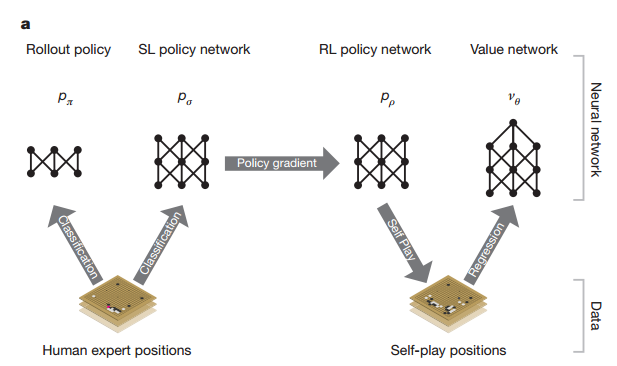
\includegraphics[width=\hsize]{example/net.png}
	\bicaption[这里将出现在插图索引]
	{深度学习网络组成}
	{Neural network training pipeline}
	\label{fig:net}
\end{figure}
首先利用人类专家数据进行训练如下两个网络:基于快速走子策略的${\rho _\pi }$网络,这是一个浅层的快速网络用来给蒙特卡洛搜索树的模拟阶段提供评估信息,相当于是一个多分类的问题。其输入是当前局面信息,输出是各个位置的落子概率。基于监督学习的深层网络${\rho _\sigma }$,相对于rollout policy网络这个网络更加深层,拟合能力更强,相对速度更慢,这个网络是为后面前后学习策略网络初始化参数信息,同时为蒙特卡洛搜索树中在动作选择时提供先验的动作概率。
接着基于强化学习原理,建立两个网络,一个是基于策略的${\rho _\rho }$网络,和历史经验池中的网络进行相互博弈,最大化自己的奖励输出。一个是基于状态价值的${v_\theta }$网络,这个是基于前面博弈数据利用回归的原理进行建立的。在这里,策略网络和价值网络输入都是原始的棋盘信息,策略网络输出的是每个可以落子位置的概率,概率越大代表当前选手得分越高,这个网络也相当于是一个多分类网络,通过不断和自己经验池中的其他网络进行自我博弈来提升效果。价值网络输出是当前状态的评分,相当于一个回归网络。这两个网络分开进行训练如图\ref{fig:policyandvalue}
\begin{figure}[!htp]
	\centering
	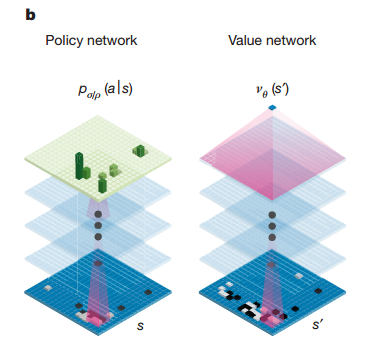
\includegraphics[width=10cm]{example/policyandvalue.png}
	\bicaption[这里将出现在插图索引]
	{策略网络和价值网络结构}
	{Neural network training pipeline}
	\label{fig:policyandvalue}
\end{figure}
\subsection{AlphaZero算法原理}
AlphaZero的出现巅峰了传统机器学习依赖大量数据的需求。根据白板理论,用专家数据学习到的结果并不一定都是可靠的,因此AlphaZero认为数据的产生不一定需要依赖人类专家数据,事实证明,这个理论效果好的超出预期:在只有8个小时的训练时间里击败了AlphaGo,又在4个小时的训练后击败了顶级国际象棋引擎Stockfish,又经过2个小时的训练后击败了日本Elmo引擎。不利用人类数据却得到了比专家方案更好的解决方案,人工智能又上了一大步。
Alphazero 相比于AlphaGo做了如下改进:
\begin{enumerate}
	\item 首先在特征的提取上面,Alphazero不再使用经过人工处理的特征,而选择原始的棋盘信心作为系统的输入,真正实现了端到端。特征提取工作直接由深度学习网络进行。
	\item 在蒙特卡洛树快速走子策略的时候,不再使用随机走子,或者利用专家数据训练快速走子策略,而直接使用强化学习策略梯度网络进行快速走子。这样提高了蒙特卡洛树预估结果的准确性。
	\item 在网络结构层面,简化了网络形式,由于不再使用监督数据,和快速走子网络,主体网络只有策略网络和价值网络。这两个网络前期特征提取工作大同小异,所以对网络进行了合并操作,大大降低了网络的复杂度。这样以轻微增加策略网络的预测错误率为代价大大降低了价值网络预测的误差。
\end{enumerate}

。Alphazero对UCTS进行了改进,每次动作选择最大化上限置信区间:
\begin{equation}
{\rm{Q(}}\mathop s\limits^ \to  {\rm{,}}\mathop a\limits^ \to  {\rm{) + U(}}\mathop s\limits^ \to  {\rm{,}}\mathop a\limits^ \to  {\rm{)}}
\end{equation}
其中,${\rm{U(}}\mathop s\limits^ \to  {\rm{,}}\mathop a\limits^ \to  {\rm{)}} \propto \frac{{P(\mathop s\limits^ \to  ,\mathop a\limits^ \to  )}}{{1 + N(\mathop s\limits^ \to  ,\mathop a\limits^ \to  )}}$。Q是定义的叶子节点的值,将会在下面提到。

叶子节点扩展的方式也不再是基于监督学习网络得到的先验概率,而是依据强化学习网络端策略网络输出的策略概率。每个叶子节点存储了以下信息:先验概率$P(\mathop s\limits^ \to  ,\mathop a\limits^ \to  )$,访问次数$N(\mathop s\limits^ \to  ,\mathop a\limits^ \to  )$,行动价值$Q(\mathop s\limits^ \to  ,\mathop a\limits^ \to  )$。
在模拟过程,每遍历一条边更新统计数据,访问次数${N(\mathop s\limits^ \to  ,\mathop a\limits^ \to  )} +=1$,更新行动价值:$Q(\vec{s},\vec{a})=\frac{1}{N(\vec{s},\vec{a})}\sum_{\vec{s}'\vert \vec{s},\vec{a}\Rightarrow \vec{s}'}V(\vec{s}')$, 其中$\vec{s}'\vert \vec{s},\vec{a} \Rightarrow \vec{s}'$表示模拟过程中从$\vec{s}$走到$\vec{s}'$的所有落子行动$\vec{a}$。
在回溯的阶段,
根据UCT算法向下遍历叶子节点,直到得到最后的结果,进行回溯操作。
在网络结构上,使用一分为二的形式,即前期特征提取部分使用相同的网络结构,因为策略网络输出的是多分类问题,所以最后一层用全连接加softmax函数,损失函数为交叉熵。而价值网络是回归问题,最后一层用sigmoid函数,损失函数为均方误差损失函数。拟合的数据就是前期蒙特卡洛搜索树搜索得到的结果。
把蒙特卡洛树和深度学习网络组合在一起的示意图如下\ref{fig:Alphazero1}:

\begin{figure}[!htp]
	\centering
	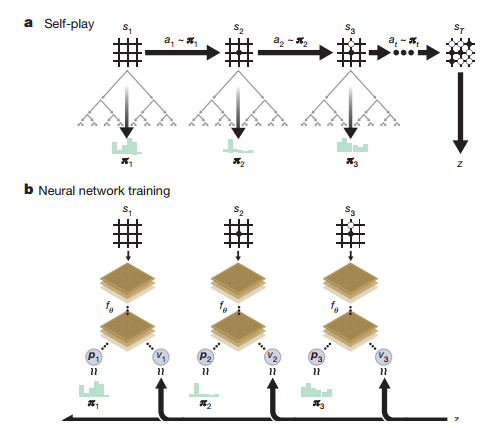
\includegraphics[width=10cm]{example/Alphazero1.png}
	\bicaption[这里将出现在插图索引]
	{AlphaZero 模型示意图}
	{Neural network training pipeline}
	\label{fig:Alphazero1}
\end{figure}
通过蒙特卡洛树得到每个状态下的$({s_t},{\pi _t},{z_t})$,其中$s_t$表示$t$时刻的状态信息,$\pi_t$表示$t$时刻蒙特卡洛搜索树的动作分布,定义为:
\begin{equation}
\label{eq:fenbu}
{\pi _{\rm{t}}}(a|{s_t}) = \frac{{N({s_{\rm{t}}},a)}}{{\sum\nolimits_b {N({s_t},b)} }}
\end{equation}
最后神经网络拟合的损失函数如下:
\begin{equation}
l = {(z - v)^2} - {\pi ^T}\log p + c{\rm{||}}\theta {\rm{|}}{{\rm{|}}^2}
\end{equation}
其中$v$和$p$分别是策略价值网络输出的评分值和动作概率值。
\section{一种改进的AC强化学习算法}
正如经典算法提到,强化学习面临的主要问题是探索和利用的平衡问题,当探索能力越强,对应的搜索树的宽度越深,利用能力越强,树的深度越深,最后结果可能会陷入局部最优解。在AlphaZero中利用了UCTS算法进行动作的选择,算法主要思想就是指导动作选择的概率。在本章对UCTS动作选择部分进行了改进,引入随机噪声,鼓励动作选择更多没有访问的节点,避免陷入局部最优的可能性。同时在神经网络的拟合部分结合训练结果用到自适应学习率的方法,加快网络前期的训练过程,在越接近最优解时缩小学习率。
算法整体示意图如图\ref{fig:ACgaijin}所示。
\begin{figure}[!htp]
	\centering
	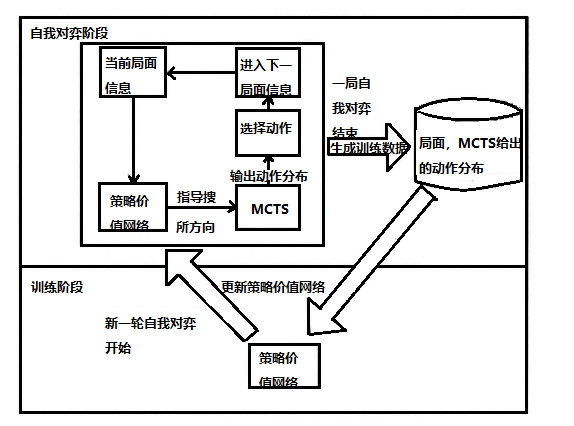
\includegraphics[width=10cm]{example/Alphazero.png}
	\bicaption[这里将出现在插图索引]
	{改进AC算法工作示意图}
	{Neural network training pipeline}
	\label{fig:ACgaijin}
\end{figure}
可见数据流的流向是先由蒙特卡洛树搜索得到相应的动作概率以及得分数据,然后把数据传向深度学习网络。由于自对抗生成式数据生成过程比较缓慢,提高样本利用率,有效平衡探索和利用的关系对于模型的效果有重要的作用。本节提出了两点改进,一是在神经网络学习阶段用自适应学习率的方法适应数据前期不稳定,后期接近标签奖励明确的特点,二是在统计蒙特卡洛搜索树信息中引入温度常数和噪声系数,促进前期探索后期利用的学习过程。
\subsection{基于交叉熵信息的自适应学习率}
在原来的Alphazero论文算法中,学习率的算法是根据迭代次数进行调整,寻求最优解的方式为异步随机梯度下降法,初始化的学习率为$\alpha$,当迭代次数为$T$时递减一半,为$2T$时再次递减,直到寻得最优解,这样学习率$\alpha$以及时间$T$都需要人为进行选取,当参数选取不合适很容易导致梯度不稳定过拟合或欠拟合现象的出现。而且迭代次是并不一定能直接反应出网络梯度更新效果的好坏,调参负担重导致结果容易出现崩溃的现象。这里我们选取能够直接反应网络更新前后变化量大小及效果的距离度量--相对熵作为衡量是否需要调整步长的指标。相对熵的定义如下:
\begin{equation}
{\rm{D}}(P{\rm{||Q}}){\rm{ = }}\sum\limits_{x \in X} {p(x)\log \frac{{P(x)}}{{Q(x)}}} 
\end{equation}

这里根据相对熵的变化自适应调整学习率,由于交叉熵能够直接反映出网络结构对策略拟合能力的好坏,当相对熵变化大于一定阈值后,说明更新前后的网络有了较大的改变,通常我们希望网络能够缓慢逐步向需要更新的方向进行改变,这时候可以适当减小学习率,反之,当交叉熵变化小于一定的阈值说明网络更新梯度过于平稳,为了提高收敛速度,可以适当加大学习步长。结合强化学习网络,定义前后差距为:
\begin{equation}
\label{eq:dist}
dist =  - \sum\limits_{i = 1}^{|A|} {{p_{\bar \theta }}(s)(\log ({p_\theta }(s)) - \log ({p_{\bar \theta }}(s))} )
\end{equation}

这里,$p_{\bar \theta}$代表状态更新前的网络参数,$p_\theta $代表状态更新后的网络参数,式\ref{eq:dist}代表了网络更新前后的变化程度相对于原来网络的变化程度。因此可以根据这个变化程度自适应调整学习率:
\begin{equation}
\label{eq:r}
r = \left\{ {\begin{array}{*{20}{c}}
	{r/\lambda ,dist > threshold\_up}\\
	{r,others}\\
	{r*\lambda ,dist < threshold\_down}
	\end{array}} \right.
\end{equation}
其中,$\lambda$代表每次更新学习率放缩的比例,$threshold\_up$和$threshold\_down$分别代表了上限阈值和下限阈值。
\subsection{引导式对弈探索}
为了进一步解决强化学习探索和利用的平衡问题,式\ref{eq:fenbu}已经介绍了经过蒙特卡洛搜索树搜索后统计的状态动作概率值,考虑到动作选择的概率很大程度依靠于蒙特卡洛树多次模拟得到的统计结果,在网络训练初期,很多时候蒙特卡洛的动作选择是随机性的,对神经网络的拟合借鉴性不大,而在网络后期,越接近奖励的步骤目标越明确,这时候可以增大对应的借鉴比例。这里引入温度常量$\tau $,动作概率公式变为:
\begin{equation}
\label{eq:gailu}
{\pi _t}(a|{s_t}) = \frac{{{e^{N{{({s_t},a)}^{1/\tau }}}}}}{{{e^{\sum\nolimits_b {N{{({s_t},b)}^{^{1/\tau }}}} }}}}
\end{equation}
在这里${N({s_t},a)}$是在状态$s_t$时选择动作$a$的次数,${\sum\nolimits_b {N{{({s_t},b)}^{1/\tau }}} }$是在状态$s_t$时,选择所有动作的总次数,这里面温度常数$\tau>0$,是控制探索和利用平衡的指标,$\tau$越小,代表动作策略更倾向于选择访问次数多的动作,当$\tau$趋近于零时函数趋近于仅利用,$\tau$越大,动作概率趋近于选择更多未探索到的策略,$\tau$趋近于正无穷,策略趋近于仅探索。这里可以在开局把$\tau$设为一个较大的初值,鼓励智能体探索不同情况的动作,在训练的后期,令$\tau  \to 0$,当训练策略稳定后,智能体将选择访问次数较多的动作。
这里为了进一步增加探索的几率,对动作概率引入随机噪声:
\begin{equation}
\label{eq:zaosheng}
	P({s_t},a) = (1 - \varepsilon ){\pi _t}(a|{s_t}) + \varepsilon {\eta _a}
\end{equation}
其中,${\pi _t}(a|{s_t})$即为\ref{eq:gailu}中的动作概率值。${\eta _a} \sim {\rm{Dir}}(c)$中$c$为狄利克雷噪声(Dirichlet noise)中的常数,$\varepsilon$为平衡噪声和概率值的常数。
所以改进后的自适应学习率调整的算法流程如下:
\begin{algorithm}[!htpb]
	\caption{基于相对熵的自适应学习率强化学习算法}% Ëã·¨±êÌâ
	\begin{algorithmic}[1]
		\Require ~~ \\
		初始学习率$r_0$,上限阈值$threshold\_up$和下限阈值$threshold\_down$,调整率$\lambda$,网络初始参数$\theta_0$,以及温度常数$\tau$和狄利克雷常数$c$,平衡系数$\varepsilon $。
		\While {没有达到网络优化停止准则}
		\State 从经验池中采样m个样本${\rm{\{ }}{{\rm{x}}^{(1)}}{\rm{,}}{{\rm{x}}^{(2)}}{\rm{,}}...{\rm{,}}{{\rm{x}}^{(m)}}{\rm{\} }}$
		\State 根据式\ref{eq:gailu}统计在$t$时刻状态$s_t$下选择不同动作的概率。
		\State 根据\ref{eq:zaosheng}更新概率值。
		\State 当利用神经网络进行概率值拟合时,根据式\ref{eq:dist}计算网络参数更新前后相对变化量。
		\State 然后利用式\ref{eq:r}更新学习率。进行下一轮蒙特卡洛树的更新和神经网络参数的更新
		\EndWhile
	\end{algorithmic}
\end{algorithm}
\section{针对五子棋双人博弈场景进行模型性能分析}
在本章,主要针对上一节提出的两点改进算法进行模型参数性能的分析,根据分析曲线和具体的应用场景进行参数的选择。由于研究的是博弈式游戏策略,因此以五子棋为实验背景进行多组对比实验。

\subsection{数据及场景介绍}
五子棋是大家耳熟能详的简单棋类游戏,其游戏规则比较简单,在一个$n\cdot n$的棋盘里,黑手和白手交替进行一次落子,可落子的空间为全盘,所以在搜索树的每一层节点都有n*n种可能性。当玩家首先在棋盘中在横向纵向以及对角上连成连续的五个棋子即判定为获胜。
抽象成强化学习模型,为了表示黑白双方的位置信息,这里用4层的8*8的棋盘表示落子信息。第一层为当前玩家全部落子位置,有子的位置为1,没有子的位置为0,同样的,第二层表示对方玩家全部落子位置,第三层为对手最后一步落子的位置,在这一层特征中只有一个位置为1,剩下位置都为0。由于是极小极大化的过程所欲需要最后一层平面表示当前玩家是黑方还是白方,黑方为全1的矩阵,白方为全0的矩阵。在动作方式的建立上,由于棋盘可落子范围为全盘,所以初始化动作为8*8的概率矩阵,当某一位置以落子,将该位置从动作池中抽掉。由于五子棋是有严格胜负规则的游戏,所以奖励可以根据游戏的胜负规则来确定:如果进行到游戏的最后如果当前玩家获胜,奖励为+1,对手奖励为-1,反之如果当前玩家失败,奖励为-1,对手为+1,如果棋盘全满,双方无子可落,双方平局,奖励全部为0。
在利用深度学习网络进行前期特征提取时,所有实验都用4层卷积网络进行特征的提取工作,在输出中,策略网络看成多分类问题激活函数选用softmax函数,价值网络看成回归问题,输出函数用tanh函数。
每下一步用400次蒙特卡洛仿真,经过self-play形式进行博弈数据的生成,把数据放进经验池中,由于五子棋棋盘信息是严格对称的,而博弈数据的产生又是比较缓慢的,所以这里采用对期棋盘数据分别进行90度,180度,270度的翻转操作,这样有效进行了数据扩充,弥补了随机采样带来的样本利用率低的缺点。
\subsection{参数对模型效果影响曲线}
在这一节对比了不同温度参数,不同噪声系数对实验结果的影响。可以通过计算策略网络的信息熵反应策略网络决策的分布离散程度,当信息熵越小,代表策略越明确,当信息熵越大,代表决策过程越趋向于随机。同时监控了神经网络的损失函数随迭代次数变化曲前,当损失函数呈下降趋势说明网络是趋近于收敛的,下降的越平滑说明网络越稳定。
首先对比不同$r$值对各种参数的影响,如图所示:
%\begin{figure}[!htp]
%	\centering
%	\begin{subfigure}{2.5cm}
%		\centering
%		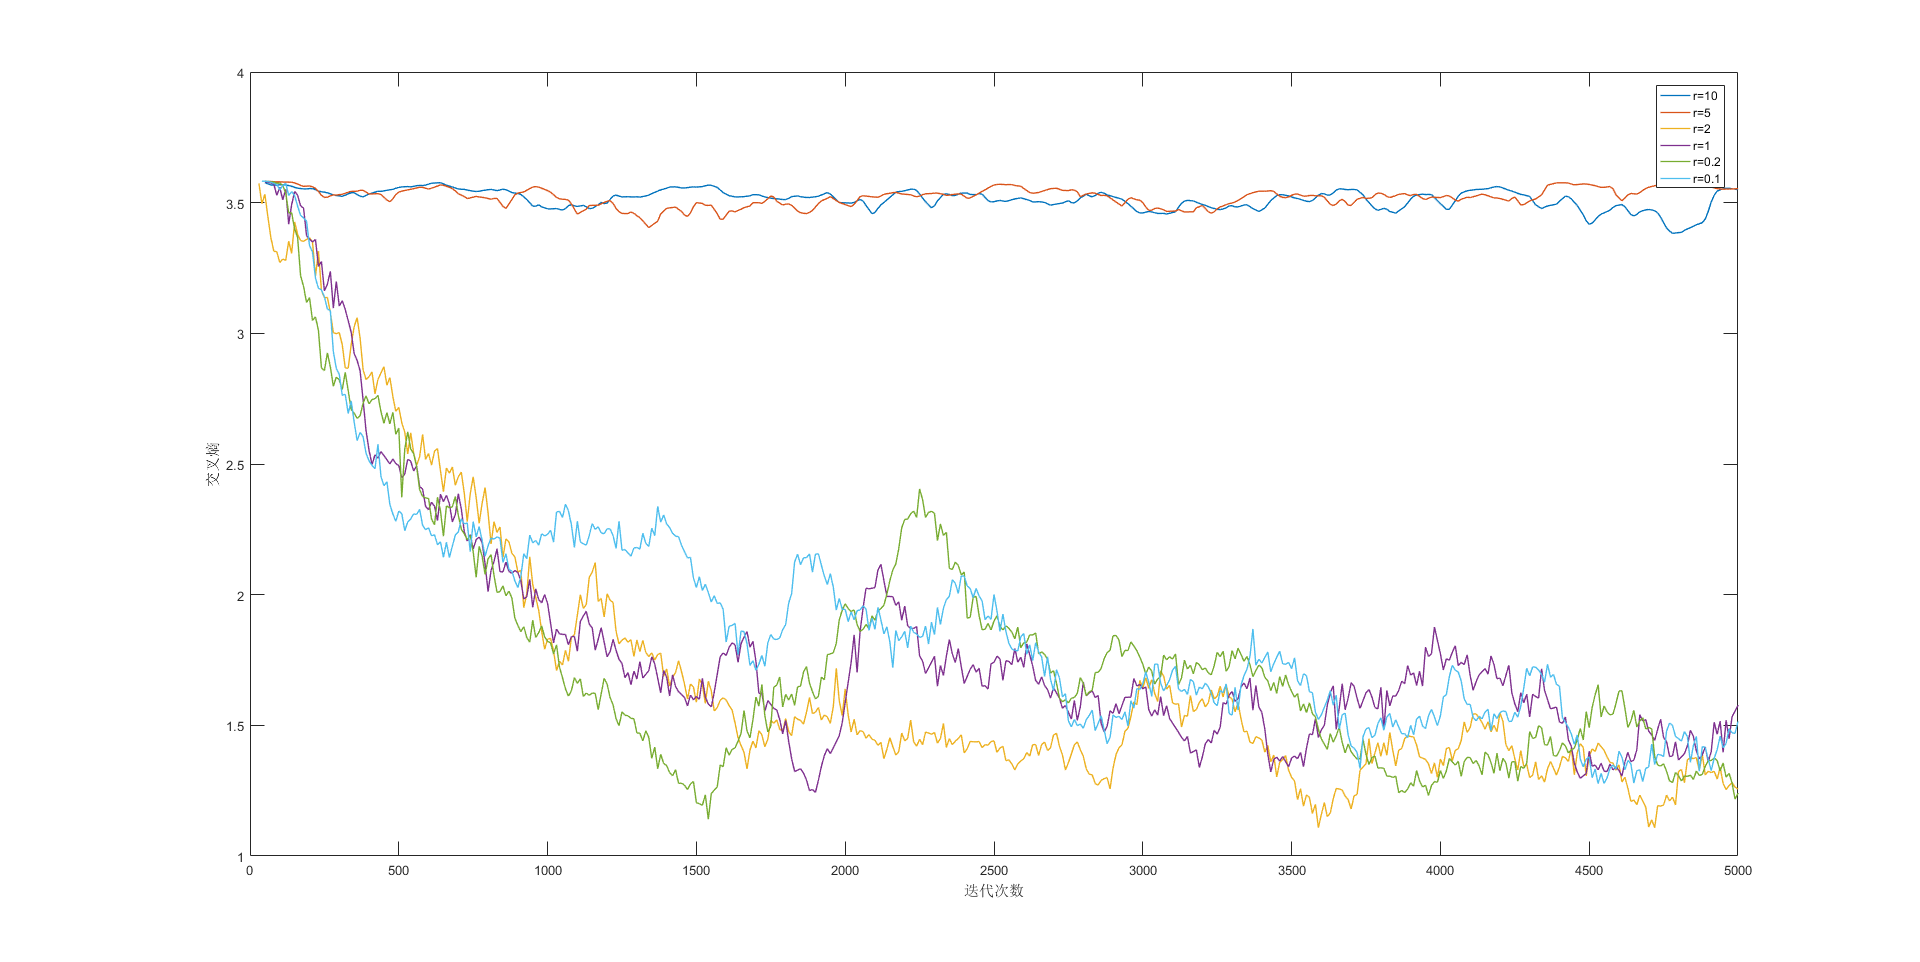
\includegraphics[height=5cm]{example/r-entropy.png}
%		\caption{学习率对交叉熵的影响}{}
%	\end{subfigure}
%	\hspace{4em}
%	\begin{subfigure}{2.5cm}
%		\centering
%		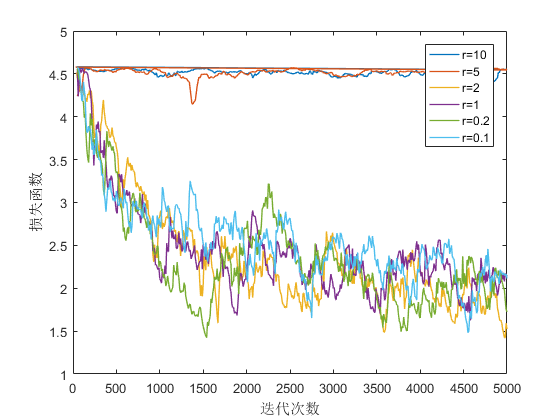
\includegraphics[height=5cm]{example/r-loss.png}
%		\caption{学习率对损失函数的影响}{}
%	\end{subfigure}
% 	\hspace{4em}
% 	
% 	\begin{subfigure}{2.5cm}
% 		\centering
% 		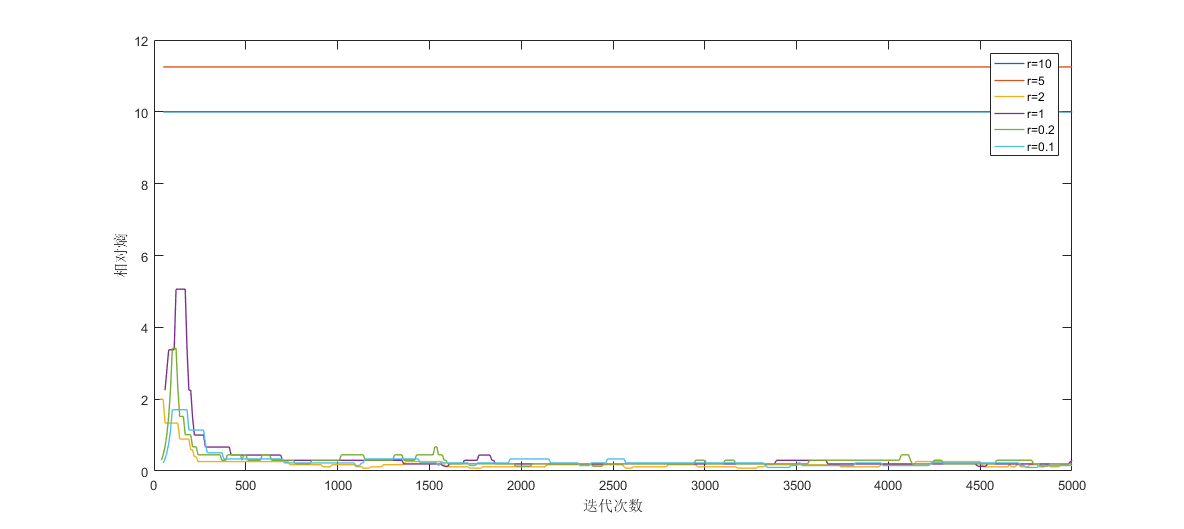
\includegraphics[height=5cm]{example/r-kl.png}
% 		\caption{学习率对相对熵的影响}{}
% 	\end{subfigure}
% 	\begin{subfigure}{2.5cm}
% 		\centering
% 		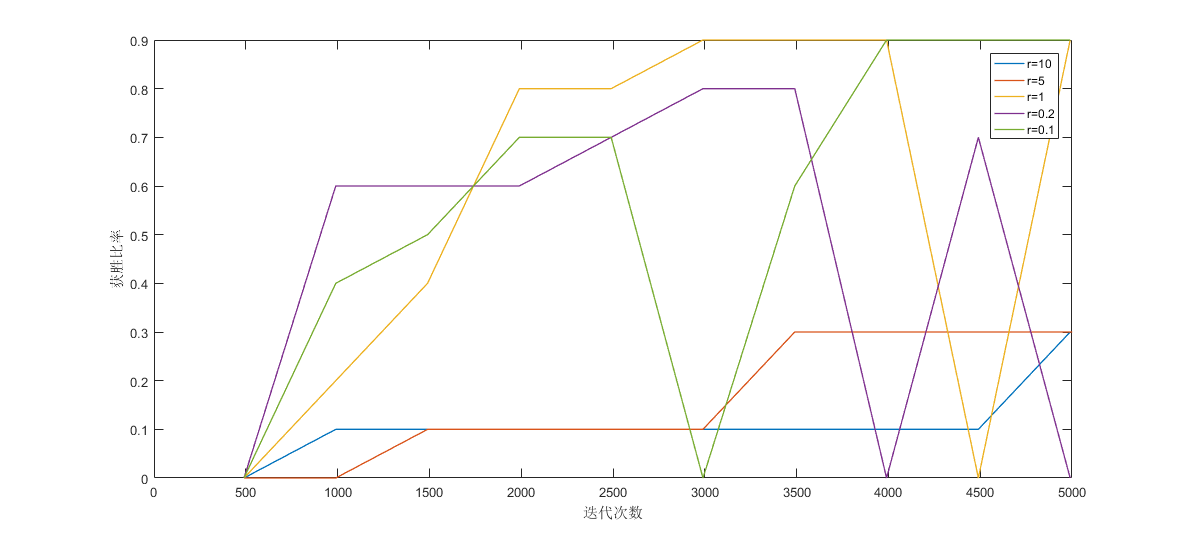
\includegraphics[height=5cm]{example/r-winratio.png}
% 		\caption{学习率对获胜率的影响}{}
% 	\end{subfigure}
%	\bicaption{学习率对不同参数的影响}{}
%	\label{fig:r}
%\end{figure}
%


\begin{figure}[t]
	\centering
	\subcaptionbox{学习率对交叉熵的影响\label{fig1:response:a}}
	{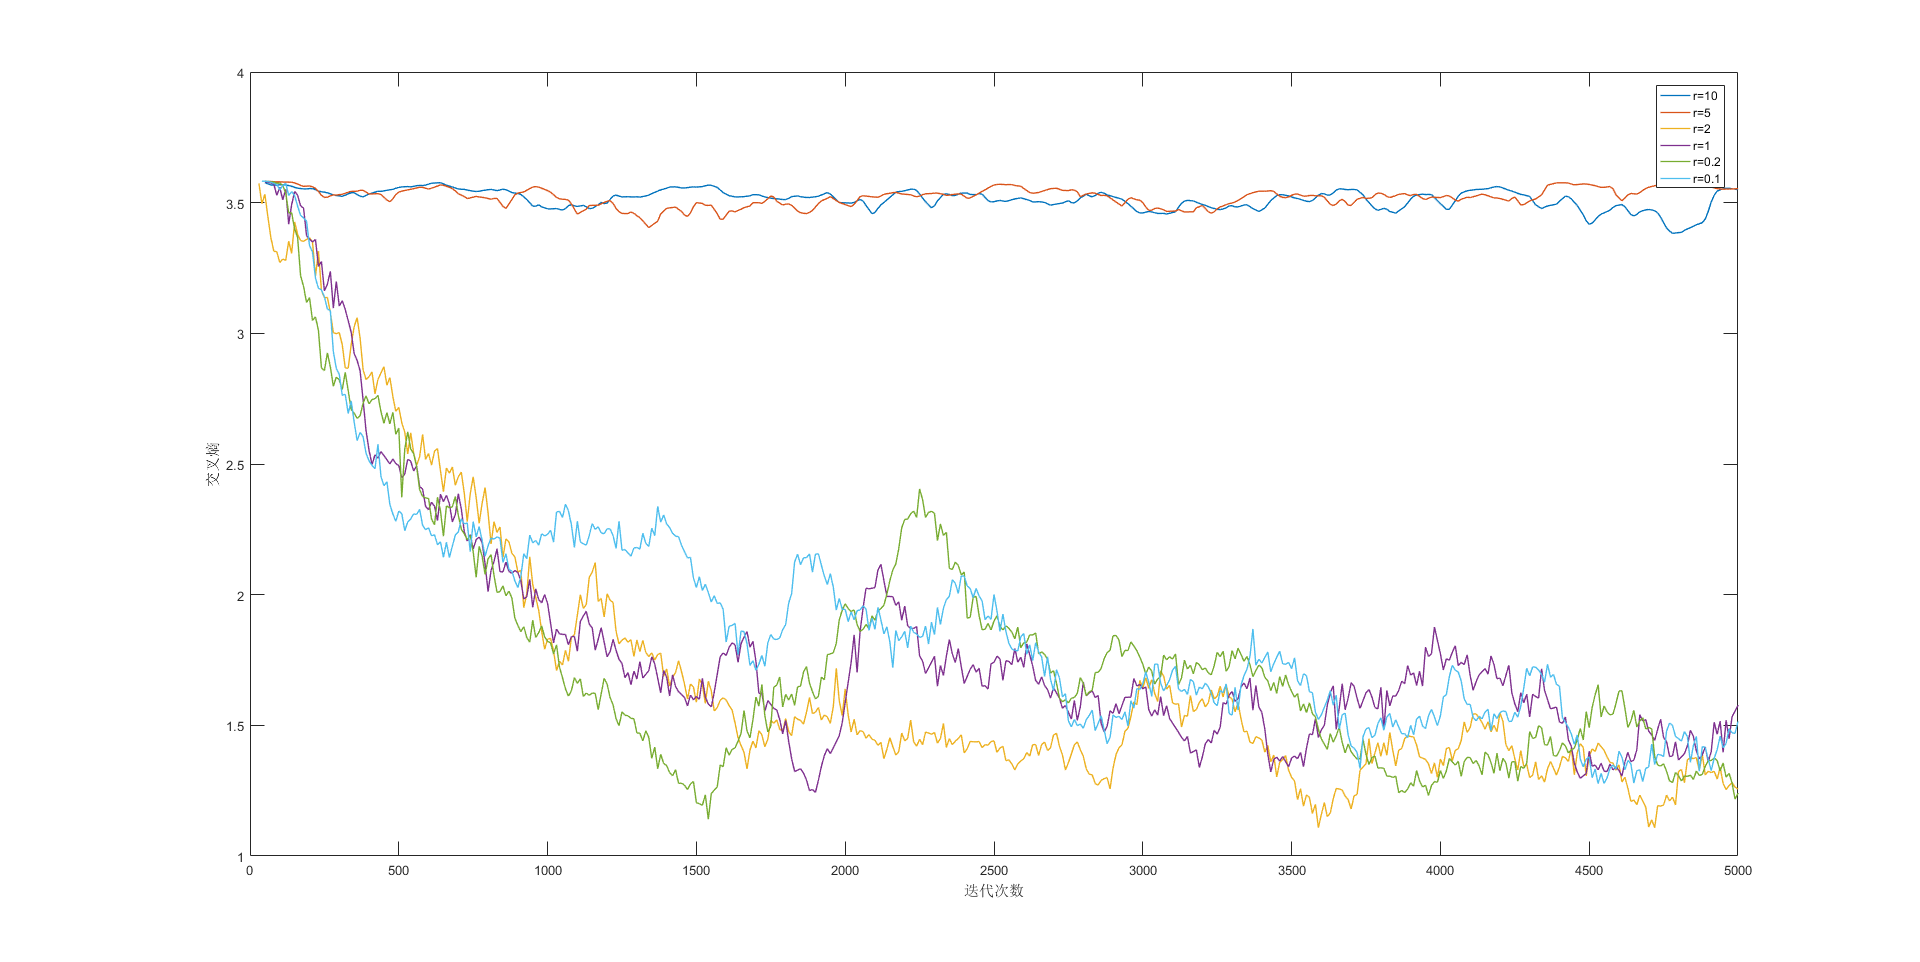
\includegraphics[width=0.45\hsize,height=0.45\hsize]{example/r-entropy.png}}
	\hspace{0.5em}
	\subcaptionbox{学习率对损失函数的影响\label{fig1:response:b}}
	{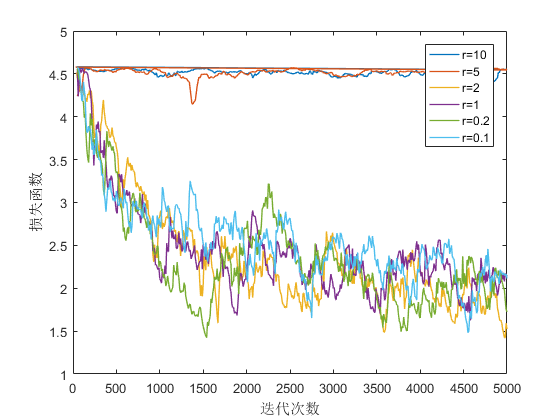
\includegraphics[width=0.45\hsize,height=0.45\hsize]{example/r-loss.png}}
	\newline
	\centering
	\subcaptionbox{学习率对相对熵的影响\label{fig1:response:c}}
	{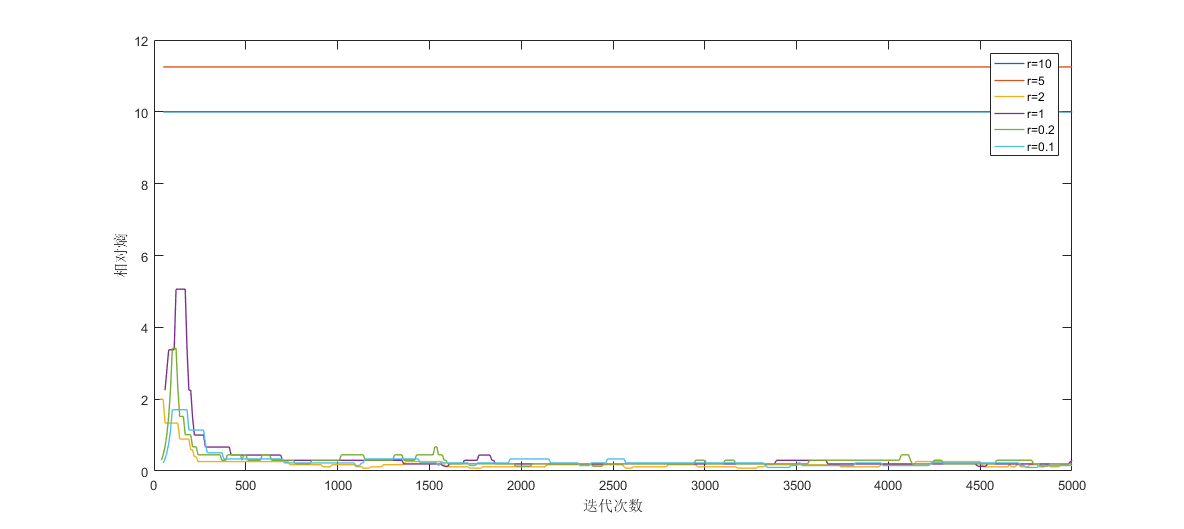
\includegraphics[width=0.45\hsize,height=0.45\hsize]{example/r-kl.png}}
	\hspace{0.5em}
	\subcaptionbox{学习率对获胜率的影响\label{fig1:response:d}}
	{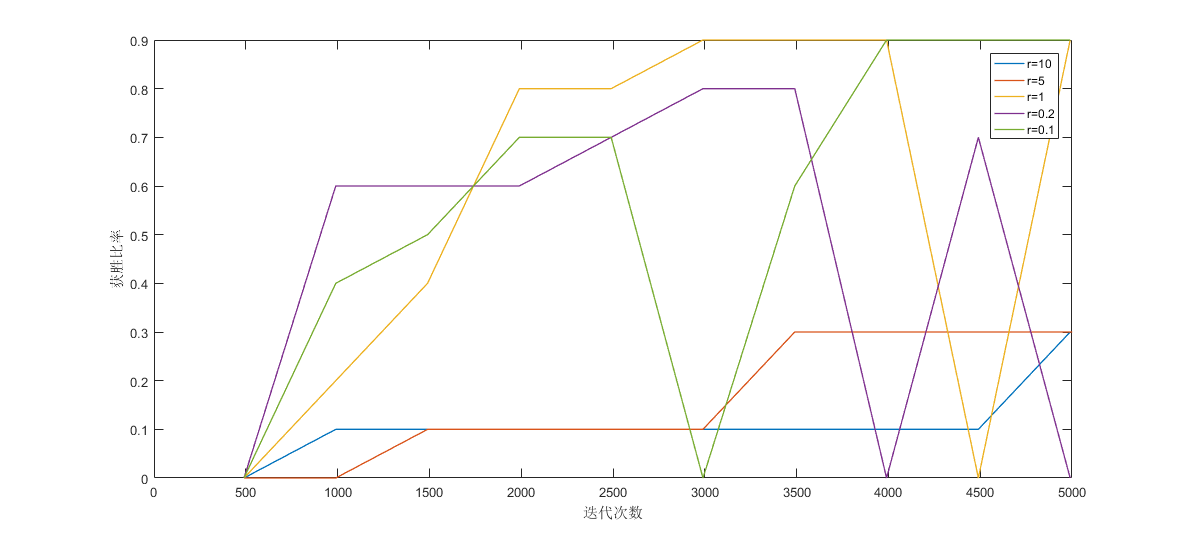
\includegraphics[width=0.45\hsize,height=0.45\hsize]{example/r-winratio.png}}
	\bicaption
	{学习率对不同参数的影响}
	{Examples of response maps during occlusions and not.The first row shows the original and response maps with no occlusions while the second row shows the maps with occlusions. The first column are the shots of sequence bear front in Princeton dataset. The color response maps are in the second column while the depth’s are in the third.}
	\label{fig1:response}
\end{figure}
图\ref{fig1:response:a}展示了不同学习率下策略网络的交叉熵,代表了策略的离散程度。图\ref{fig1:response:b}展示了损失函数随迭代次数的改变,损失函数包括策略网络损失函数和价值网络损失函数,损失函数越小代表网络拟合self-play数据效果越好。图\ref{fig1:response:c}代表了网络参数的相对变化情况,自适应调整学习率时,根据相对熵调整学习率移动方向,所以相对熵稳定在一个相对小值利用模型学习。图\ref{fig1:response:d}代表在训练过程中智能体和一个提前训练好的用rollout策略学习的智能体进行博弈的结果,网络每迭代500次进行一次评估,对战10回合统计获胜比率。
一个好的网络应该交叉熵随着迭代的进行呈下降趋势。当$r$过大时,交叉熵基本不变网络相当于随机输出动作,当$r=10$和$r=5$时可以看出智能体在随机输出动作,神经网络的损失函数没有呈下降的趋势,从获胜比例看获胜率相抵很低。固定迭代次数,交叉熵和损失函数随着学习率减小而减小。但并不是$r$越小越好,当$r=0.1$时从获胜比率看智能体模型并不稳定。

\begin{figure}[t]
	\centering
	\subcaptionbox{温度常数对交叉熵的影响\label{fig2:response:a}}
	{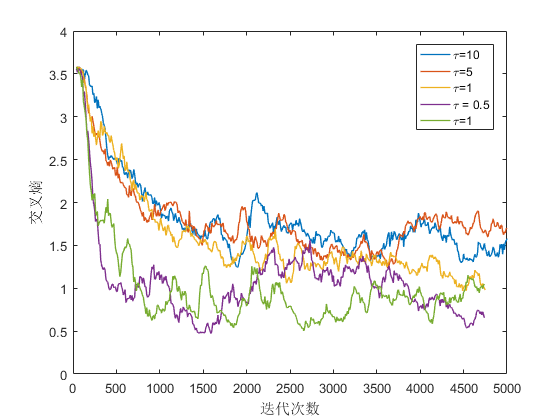
\includegraphics[width=0.45\hsize,height=0.45\hsize]{example/temp-entropy.png}}
	\hspace{0.5em}
	\subcaptionbox{温度常数对损失函数的影响\label{fig2:response:b}}
	{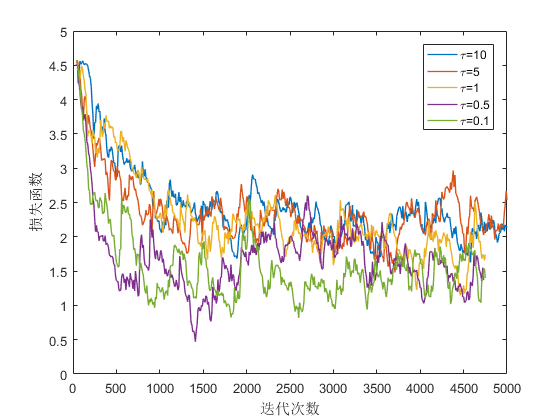
\includegraphics[width=0.45\hsize,height=0.45\hsize]{example/temp-loss.png}}
	\newline
	\centering
	\subcaptionbox{温度常数对相对熵的影响\label{fig2:response:c}}
	{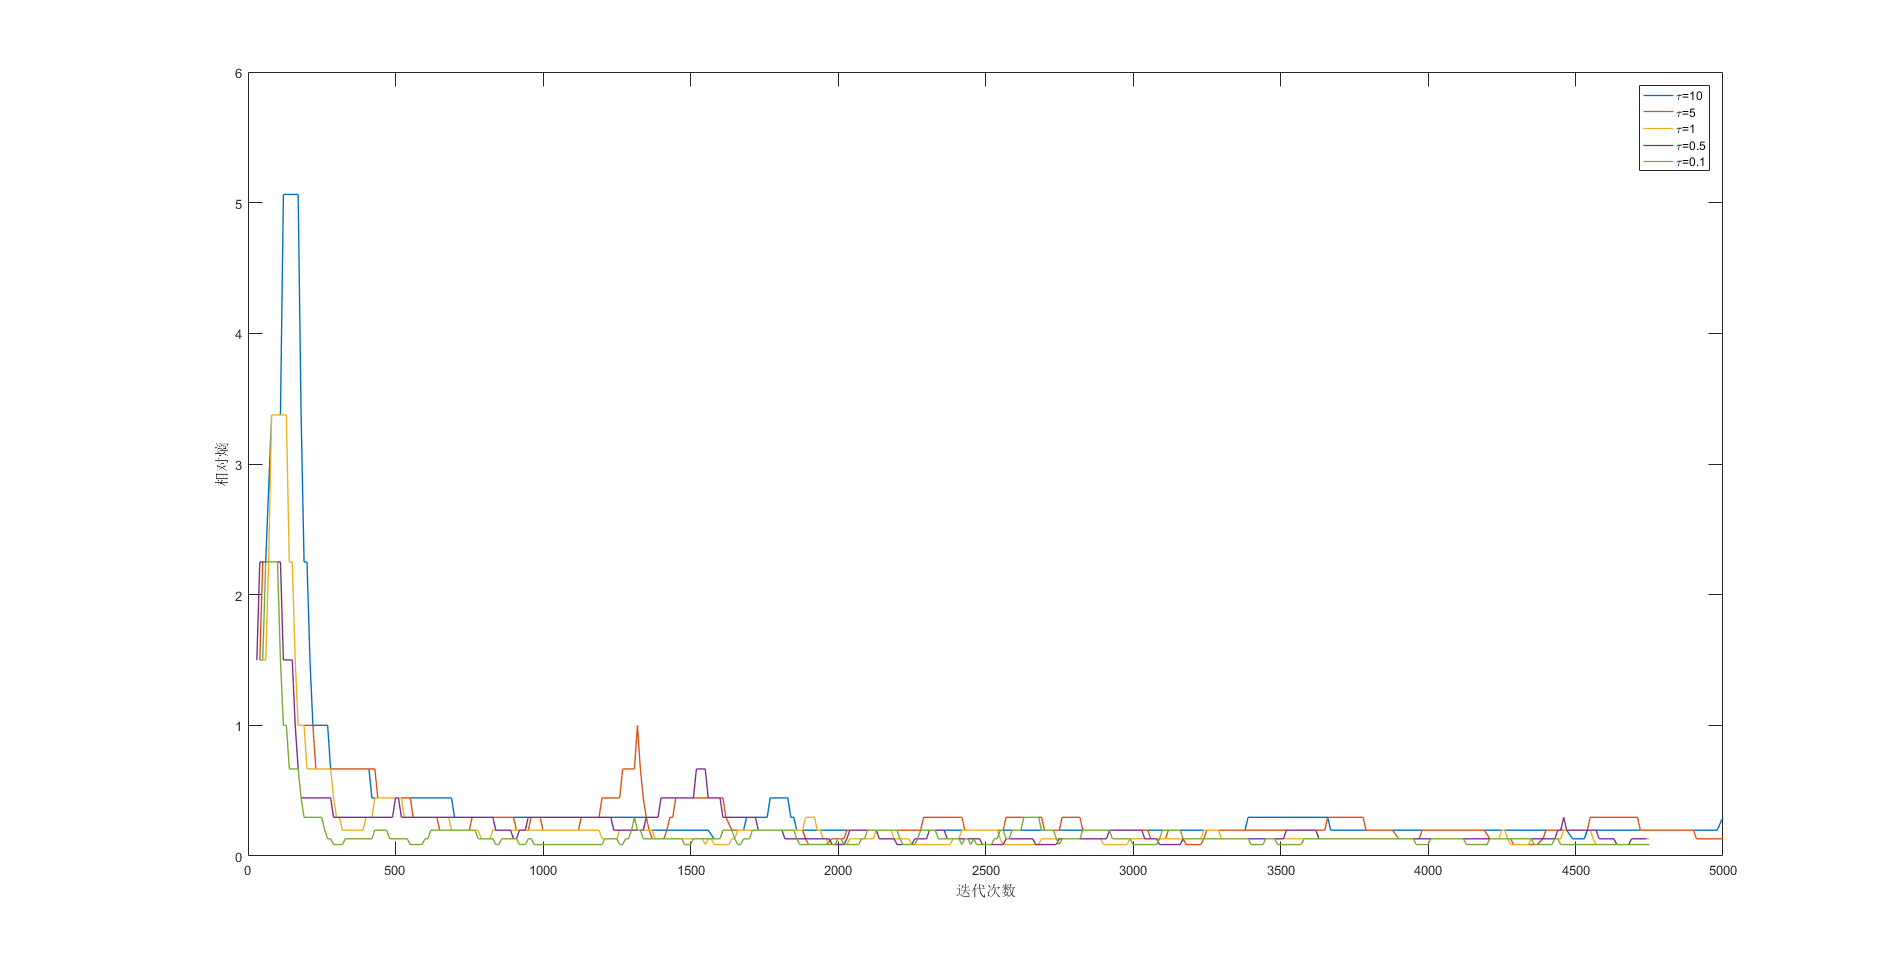
\includegraphics[width=0.45\hsize,height=0.45\hsize]{example/temp-kl.png}}
	\hspace{0.5em}
	\subcaptionbox{温度常数对获胜率的影响\label{fig2:response:d}}
	{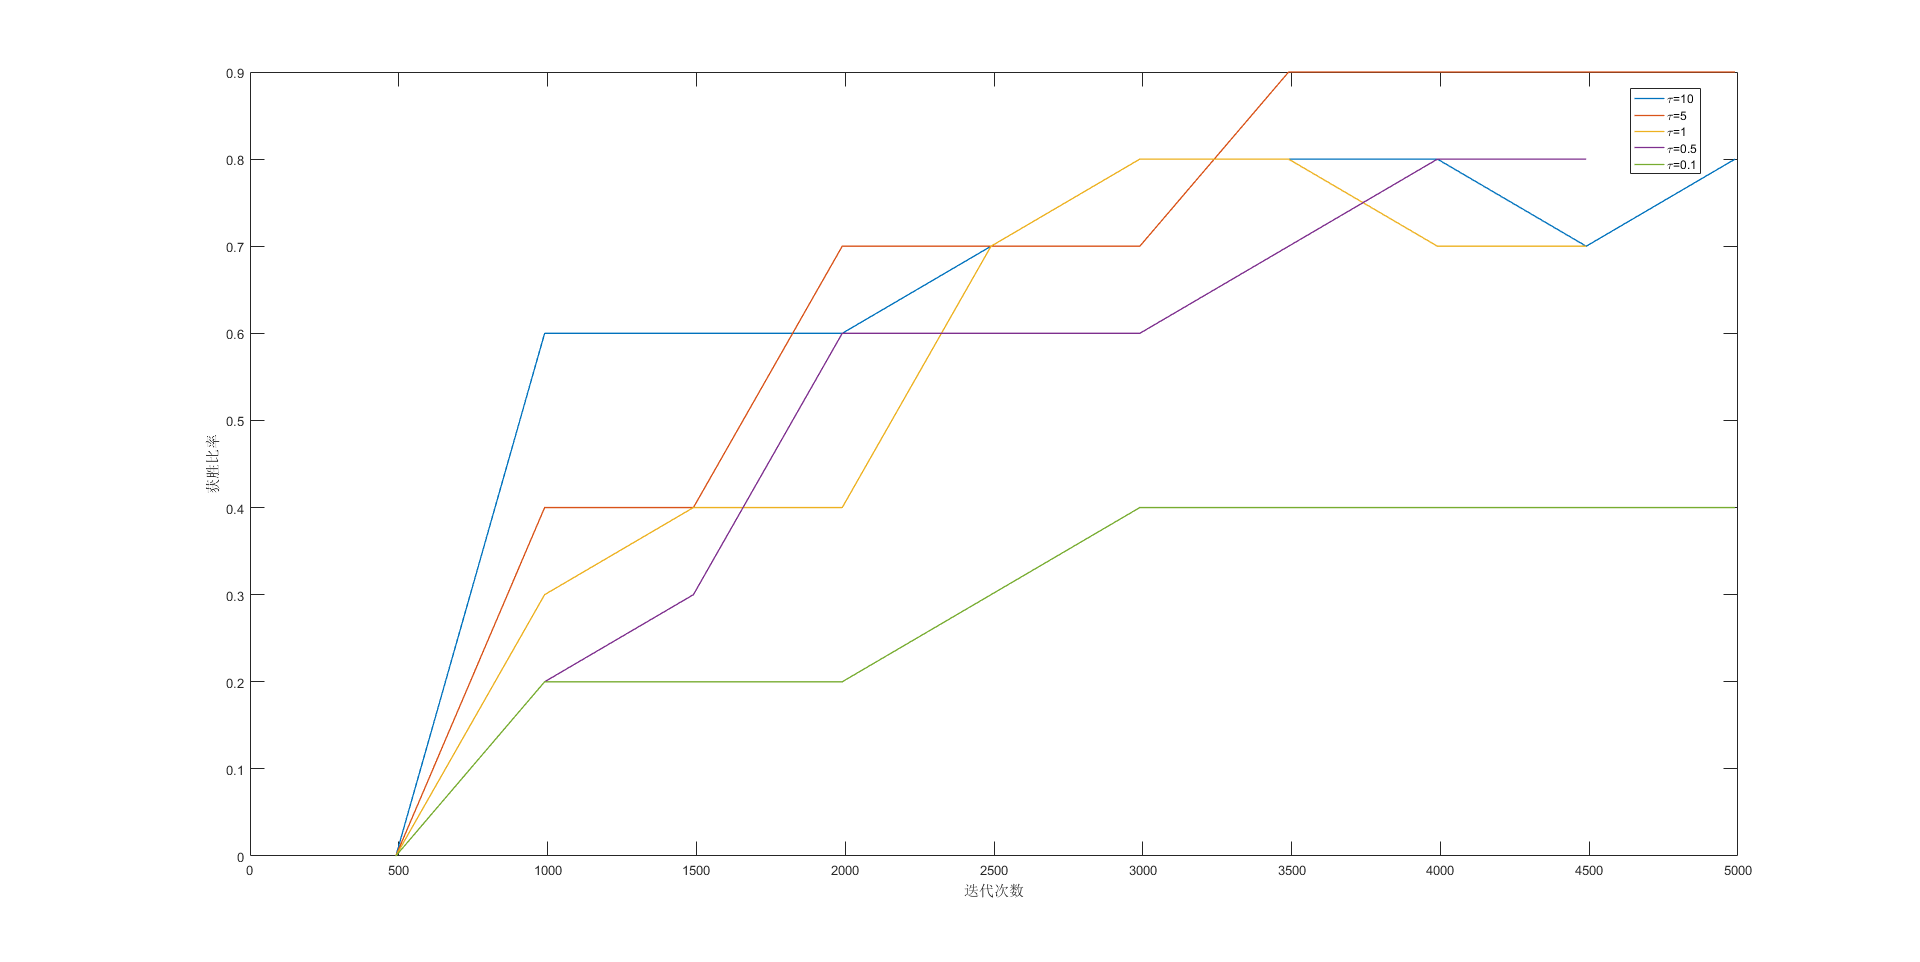
\includegraphics[width=0.45\hsize,height=0.45\hsize]{example/temp-winratio.png}}
	\bicaption
	{温度常数对不同参数的影响}
	{Examples of response maps during occlusions and not.The first row shows the original and response maps with no occlusions while the second row shows the maps with occlusions. The first column are the shots of sequence bear front in Princeton dataset. The color response maps are in the second column while the depth’s are in the third.}
	\label{fig2:response}
\end{figure}
图\ref{fig2:response}展示了温度常数对不同参数的影响,这里面仍以交叉熵,相对熵,损失函数和获胜比率进行对比。
可以看出来,$\tau$越大,策略网络趋向于探索策略,交叉熵下降缓慢,以$\tau=10$为例,从损失函数看,其损失函数下降缓慢,收敛较慢,从获胜率曲线看,其前期表现较其他参数快,因为前期蒙特卡洛搜索得到的结果并不可靠,单纯拟合网络并不是最好的结果,但是由于动作的不稳定性,随着迭代次数增加其获胜率上升比较缓慢。温度系数越小,策略越趋向于仅利用,损失函数下价格呢的会很快,交叉熵也下降的比较快,相当于贪心策略。但是从$\tau=0.1$曲线的获胜率来看,其后期表现很差。所以合理平衡探索和利用对于强化学习问题来说是很重要的。
\section{基于五子棋的单智体博弈实验}

在上一节参数选择经验的基础上,这里我们选取参数信息进行不同算法之间结果比较。本实验对训练过程中神经网络的损失函数信息,学习率,总损失,以及策略端损失和价值网络损失进行对比,证明算法的可行性。策略网络损失代表神经网络动作部分和蒙特卡洛树拟合值的偏差,价值网络代表神经网络和真实值之间回归的偏差,网络优化的总损失函数为策略损失和价值损失之和。这里具体把两个损失函数分开,看不同算法得到的网络模型效果对比。在这里参数信息如下:
\begin{table}
	\centering
	\caption{股票数据回归结果}
	\begin{tabular}{c|c}
		\hline 
		棋盘大小 & 8*8 \\ 
		\hline 
		自适应学习率参数 & 1.0 \\ 
		\hline 
		温度探索参数temp & 1.0 \\ 
		\hline 
		每次落子蒙特卡洛搜索次数 & 400 \\ 
		\hline 
		批训练样本大小 & 500 \\ 
		\hline 
		迭代次数 & 1500 \\ 
		\hline 
	\end{tabular} 
\end{table}


对比不同算法得到的结果:
(加不同算法的曲线图)

最后得到的五子棋模型效果如下:
在初始位置,神经网络对各个位置落子的概率如下:
可以看出,模型倾向于把初始落子位置放在中间,这也符合正常规则的五子棋的下法,第一步越靠近中间越有利。从这个角度说明了网络学习到参数的有效性。这里展示两组不同的对弈结果,下图分别是智能体自我博弈过程中的落子位置:
初始位置蒙特卡洛搜索得到的结果:

\begin{figure}[!htpb]
	\centering
	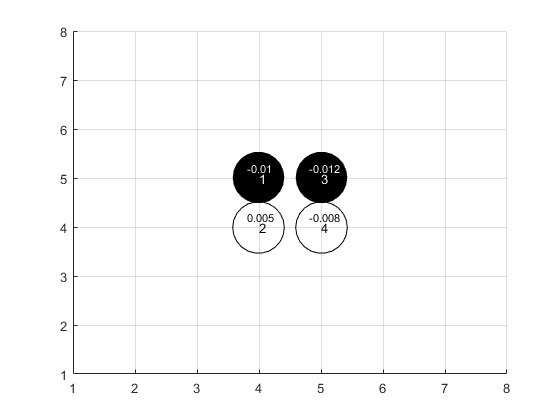
\includegraphics[width=6cm]{example/AVA1.png}
	\hspace{0.5cm}
	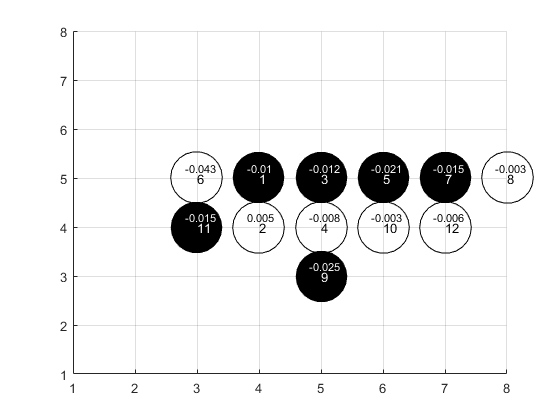
\includegraphics[width=6cm]{example/AVA2.png}
	\hspace{0.5cm}
	\includegraphics[width=6cm]{example/AVA3.png}
	\hspace{0.5cm}
	\includegraphics[width=6cm]{example/AVA4.png}
	\hspace{0.5cm}
	\includegraphics[width=6cm]{example/AVA5.png}
	\hspace{0.5cm}
	\includegraphics[width=6cm]{example/AVA6.png}
	\hspace{0.5cm}
	\includegraphics[width=6cm]{example/AVA7.png}
	\hspace{0.5cm}
	\includegraphics[width=6cm]{example/AVA8.png}
	\bicaption[这里将出现在插图索引中]
	{智能体自我博弈过程图示}
	{English caption}
	\label{fig:AIvsAI}
\end{figure}

在初始位置,神经网络对各个位置落子的概率如下:
\begin{table}[t]
	\centering
	\caption{股票数据回归结果}
\begin{tabular}{|c|c|c|c|c|c|c|c|}
	\hline 
	1.475e-4 & 1.060e-4 & 5.279e-5 & 1.107e-4 & 9.022e-5 & 4.170e-5 & 1.109e-4 & 1.193e-4 \\ 
	\hline 
	1.584e-4 & 6.658e-5 & 1.091e-3 & 5.847e-4 & 7.405e-4 & 8.547e-4 & 7.423e-5 & 8.784e-5 \\ 
	\hline 
	3.247e-5 & 7.867e-4& 4.690e-2 & 8.819e-3 & 7.429e-3&4.045e-2 & 8.091e-4 & 3.269e-5 \\ 
	\hline 
	9.957e-5& 5.741e-4 & 7.397e-3 & 0.184 & 0.198 & 0.011& 5.795e-4 & 7.367e-5 \\ 
	\hline 
	6.310e-5 &6.247e-4& 9.647e-3& 0.168 & 0.178 & 1.057e-2 & 7.635e-4 & 9.389e-5 \\ 
	\hline 
	3.174e-5 & 7.434e-4 & 4.978e-2 & 1.201e-2 & 1.064e-2 & 4.221e-2 & 6.999e-4 & 3.441e-5 \\ 
	\hline 
	1.170e-4 & 5.157e-5& 8.608e-4 & 7.298e-4 & 5.024e-4 & 9.605e-4 & 4.176e-05 & 8.261e-5\\ 
	\hline 
	1.148e-4 &7.760e-5 &  5.001e-5 & 1.053e-4 & 1.379e-4 & 2.526e-05 & 6.797e-05 & 1.110e-4 \\ 
	\hline 
\end{tabular} 
\end{table}

蒙特卡洛搜索得到的各个位置的概率:
\begin{table}[b]
	\centering
	\caption{股票数据回归结果}
\begin{tabular}{|c|c|c|c|c|c|c|c|}
		\hline 
		0& 0 & 0 & 0 & 0 & 0 &  0&  0\\ 
		\hline 
		0& 0 & 0 & 0 & 0 & 0 &  0&  0\\ 
		\hline 
		0 & 0 & 0.0125 & 0.005 & 0.0025 & 0.0125 & 0 & 0 \\ 
		\hline 
		0 & 0 & 0 & 0.1925 & 0.2425 & 0.01 & 0 & 0 \\ 
		\hline 
		0 & 0 & 0.0025 & 0.2075 & 0.265 & 0.01 & 0 & 0 \\ 
		\hline 
		0 & 0 & 0.01 & 0.005 & 0.0025 & 0.015 & 0 & 0 \\ 
		\hline 
		0 & 0 & 0 & 0 & 0 & 0 & 0 & 0 \\ 
		\hline 
		0 & 0 & 0 & 0 & 0 & 0 & 0 & 0 \\  
		\hline 
\end{tabular} 
\end{table}

可以看出,模型倾向于把初始落子位置放在中间,这也符合正常规则的五子棋的下法,第一步越靠近中间越有利。从这个角度说明了网络学习到参数的有效性。这里展示两组不同的对弈结果,下图分别是智能体自我博弈过程中的落子位置:

\begin{figure}[!htp]
	\centering
	\includegraphics[width=6cm]{example/AVH1.png}
	\hspace{0.5cm}
	\bicaption[这里将出现在插图索引中]
	{智能体自我博弈过程图示}
	{English caption}
	\label{fig:AIvsAI}
\end{figure}

在下一步蒙特卡洛树得到的统计概率为:

\begin{tabular}{|c|c|c|c|c|c|c|c|}
	\hline 
	0& 0 & 0 & 0 & 0 & 0 &  0&  0\\ 
	\hline 
	0& 0 & 0 & 0 & 0 & 0 &  0&  0\\ 
	\hline 
	0 & 0 & 0.0125 & 0.005 & 0.0015 & 0.0125 & 0 & 0 \\ 
	\hline 
	0 & 0 & 0 & 0.1925 & 0.3425 & 0.02 & 0 & 0 \\ 
	\hline 
	0 & 0 & 0.0015 & 0.205 & 0.245 & 0.01 & 0 & 0 \\ 
	\hline 
	0 & 0 & 0.01 & 0.0025 & 0.005 & 0.015 & 0 & 0 \\ 
	\hline 
	0 & 0 & 0 & 0 & 0 & 0 & 0 & 0 \\ 
	\hline 
	0 & 0 & 0 & 0 & 0 & 0 & 0 & 0 \\  
	\hline 
\end{tabular} 

可以看出策略很明确,下一步的落子信息为:

\begin{figure}[!htp]
	\centering
	\includegraphics[width=6cm]{example/AVH2.png}
	\hspace{0.5cm}
	\bicaption[这里将出现在插图索引中]
	{智能体自我博弈过程图示}
	{English caption}
	\label{fig:human2}
\end{figure}
接下来的落子信息为:
\begin{figure}[!htp]
	\centering
	\includegraphics[width=6cm]{example/AVH3.png}
	\hspace{0.5cm}
	\bicaption[这里将出现在插图索引中]
	{智能体自我博弈过程图示}
	{English caption}
	\label{fig:human3}
\end{figure}
当模型训练好后,AI的策略是选取蒙特卡洛搜索得到的最大值贪心的进行落子。图给出了接下来几步的落子信息:
\begin{figure}[!htp]
	\centering
	\includegraphics[width=6cm]{example/AVH4.png}
	\hspace{0.5cm}
	\includegraphics[width=6cm]{example/AVH5.png}
	\hspace{0.5cm}
	\includegraphics[width=6cm]{example/AVH6.png}
	\hspace{0.5cm}
	\includegraphics[width=6cm]{example/AVH7.png}
	\bicaption[这里将出现在插图索引中]
	{人机对弈过程图示}
	{English caption}
	\label{fig:AIvsHuman}
\end{figure}
%\begin{figure}[!htp]
%	\centering
%	\includegraphics[width=6cm]{example/AVH4.png}
%	\hspace{0.5cm}
%		\includegraphics[width=6cm]{example/AVH5.png}
%	\hspace{0.5cm}
%		\includegraphics[width=6cm]{example/AVH6.png}
%	\hspace{0.5cm}
%		\includegraphics[width=6cm]{example/AVH7.png}
%    \hspace{0.5cm}
%	\bicaption[这里将出现在插图索引中]
%	{智能体自我博弈过程图示}
%	{English caption}
%	\label{fig:human4}
%\end{figure}
\begin{figure}[!htp]
	\centering
	\includegraphics[width=6cm]{example/AVH8.png}
	\hspace{0.5cm}
	\bicaption[这里将出现在插图索引中]
	{智能体自我博弈过程图示}
	{English caption}
	\label{fig:human4}
\end{figure}

经过几轮对战后到达状态为图\ref{fig:human4} 第四幅图。智能体蒙特卡洛搜索得到的统计概率为:

\begin{tabular}{|c|c|c|c|c|c|c|c|}
	\hline 
	0& 0 & 0 &0  & 0 &0 0.2425 & 0 &0  \\ 
	\hline 
	0 & 0 & 0 & 0 & 0 & 0 & 0.615 & 0 \\ 
	\hline 
	0 & 0 & 0 & 0 & 0 & 0 & 0 & 0 \\ 
	\hline 
	0 & 0 & 0 & 0 & 0& 0 & 0 & 0 \\ 
	\hline 
	0 & 0 & 0.135 & 0 & 0.0025 & 0 & 0 & 0.0025 \\ 
	\hline 
	0 & 0 & 0 & 0 & 0 & 0 & 0 & 0 \\ 
	\hline 
	0 & 0 & 0 & 0 & 0 & 0 & 0 & 0 \\ 
	\hline 
	0 & 0 & 0 & 0 & 0 & 0 & 0 & 0 \\ 
	\hline 
\end{tabular}

选择概率最大的进行动作,得到如下状态:

\begin{figure}[!htp]
	\centering
	\includegraphics[width=6cm]{example/AVH9.png}
	\hspace{0.5cm}
	\bicaption[这里将出现在插图索引中]
	{智能体自我博弈过程图示}
	{English caption}
	\label{fig:human5}
\end{figure}

这时策略神经网络输出概率值信息为:

\begin{tabular}{|c|c|c|c|c|c|c|c|}
	\hline 
	4.364e-3 & 1.047e-3 & 7.525e-3 & 2.883e-3 & 6.946e-4 & 5.545e-3 & 0.057 & 0.309 \\ 
	\hline 
	3.495e-3 & 1.008e-2 & 9.739e-3 & 7.828e-05 & 1.271e-3 & 3.174e-05 & 7.719e-4 & 7.758e-4 \\ 
	\hline 
	5.235e-4 & 7.740e-3 & 6.412e-4 & 5.572e-05 & 1.263e-06 & 1.740e-4 & 3.681e-3 & 6.366e-4 \\ 
	\hline 
	7.379e-2 & 1.574e-2 & 6.703e-07 & 6.327e-06 & 3.206e-05 & 1.603e-05 & 5.863e-2 & 9.232e-3 \\ 
	\hline 
	2.077e-4 & 1.737e-05 & 1.134e-4 & 2.158e-05 & 2.920e-06 & 1.697e-4 & 5.049e-4 & 2.913e-2 \\ 
	\hline 
	9.056e-2 & 1.897e-2 & 3.469e-06 & 2.165e-3 & 2.638e-3 & 1.505e-3 & 1.165e-2 & 0.128 \\ 
	\hline 
	8.939e-4 & 2.178e-4 & 4.440e-4 & 8.316e-2 & 1.967e-3 & 8.452e-4 & 5.612e-4 & 4.942e-4 \\ 
	\hline 
	9.371e-4 & 6.839e-4 & 4.050e-3 & 3.668e-4 & 2.882e-2 & 3.848e-4 & 6.134e-4 &5.001e-4 \\ 
	\hline 
\end{tabular} 

蒙特卡洛树统计得到的概率信息为:

\begin{tabular}{|c|c|c|c|c|c|c|c|}
	\hline 
	0& 0 & 0 &0  & 0 &0  & 0.03 &0.625  \\ 
	\hline 
	0 & 0 & 0.0225 & 0 & 0 & 0 & 0 & 0 \\ 
	\hline 
	0 & 0 & 0 & 0 & 0 & 0 & 0.1 & 0 \\ 
	\hline 
	0 & 0 & 0 & 0 &0 & 0 & 0 & 0 \\ 
	\hline 
	0 & 0 &0& 0 & 0 & 0 & 0 & 0.07\\ 
	\hline 
	0 & 0 & 0 & 0 & 0.0575 & 0 & 0 & 0 \\ 
	\hline 
	0 & 0 & 0 & 0 & 0 & 0 & 0 & 0 \\ 
	\hline 
	0 & 0 & 0 & 0.0725 & 0 & 0 & 0 & 0 \\ 
	\hline 
\end{tabular}

这时观察当前状态对于黑方叶子节点预测奖励为0.97883,根据贪心策略选择概率最大的动作执行,得到下面的状态信息:

\begin{figure}[!htp]
	\centering
	\includegraphics[width=6cm]{example/AVH10.png}
	\hspace{0.5cm}
	\bicaption[这里将出现在插图索引中]
	{智能体自我博弈过程图示}
	{English caption}
	\label{fig:human6}
\end{figure}

最后黑方获胜,通过实验可知距离奖励越近策略越明确,在本实验中,观察策略网络输出的交叉熵可以看出智能体在训练过程中随着迭代的进行策略越接近于明确,损失函数不断下降。在人机博弈时,神经网络基本能准确输出各个位置获胜的概率,和蒙特卡洛树统计得到的概率基本一致。在游戏结束时,奖励越来越明确,智能体也能准确感知当前的状态信息并作出决策。在自我博弈过程中,连个智能体相互对抗直到和棋,说明训练出的智能体基本棋力相当,也证明了用自我博弈方式产生数据的有效性。由于棋盘过小,硬件资源有限,这里只给出了8*8的情况,又由于强化学习训练比较困难,稳定性不高,在本章只介绍了对于对称类棋盘博弈的相关实验,对于其他应用场景的拓展还有待开发。
\section{本章小结}
本章主要针对对称类双人棋盘博弈模型进行探索和研究。在文章的第一部分介绍了博弈模型的概念和类别,第二部分介绍了AlphaGo和AlphaZero的基本原理,其主要的组成部分有蒙特卡洛搜索树,深度学习网络和强化学习基本原理。首先利用蒙特卡洛搜索树建立两个智能体相互博弈的模型,在树的叶子节点选择过程中用到了强化学习最大化奖励函数的原理,在叶子节点扩展中需要结合深度学习网络进行动作和值函数的估计,然后把多次模拟的数据进行统计,作为深度学习网络的拟合标签,以更新后的深度学习网络为基础进行下一次树的建立。最后策略网络就是模型得到的最终结果。AlphaGo利用了人类监督数据进行网络的初始化处理以及搜索树的快速走子,AlphaZero则从无到有完全利用自我博弈数据进行深度学习网络的拟合。针对于强化学习探索和利用的平衡问题以及在深度学习网络更新中学习率难以选择的问题,在本章的第三部分提出了两点改进:受多臂老虎机模型的启发,这里用温度系数控制动作选择部分对探索和利用的平衡,避免因探索权重大带来的计算复杂度高和利用权重大带来模型陷入局部最优解的问题,为了进一步避免动作过于单一,在概率分布上加入随机噪声。用相对熵衡量策略网络输出参数的相对变化范围,根据网络参数的变化自适应调整学习率,在网络训练前期加快步长,在接近最优解时减小步长,既能提高训练效率又能避免局部最优。在文章的第四部分针对改进的方案结合五子棋模型原型讨论了在不同温度系数和不同学习率参数下网络损失函数和交叉熵的变化曲线,根据输出曲线合理选择网络的参数。在第五部分针对改进算法设计了五子棋实验,展示了人机对战结果和智能体之间自博弈结果。针对人机博弈过程详细展示了蒙特卡洛搜索树搜索结果和神经网络输出概率值,在结果上验证了改进算法的可行性。
%# -*- coding: utf-8-unix -*-
% !TEX program = xelatex
% !TEX root = ../thesis.tex
% !TEX encoding = UTF-8 Unicode
%%==================================================
%% chapter01.tex for SJTU Master Thesis
%%第五章
%%==================================================
\chapter{基于深度强化学习的飞机对抗策略}
\section{引言}
在上一章主要以双人棋盘类博弈策略进行描述,在本章将讨论非棋盘类单智能体对抗和二对二智能体对抗的问题。对于对称类棋盘游戏来说,其规则简单,并且可落子范围随着双方不断落子逐渐缩小,动作双方最多走满全盘步数即可或胜负,应用场景比较单一,对于其他应用场景还有待扩展,除此之外,现有的强化学习模型大多数针对单智能体游戏类的决策任务,对于两个以上智能体既有竞争又有合作的情况更加复杂,当对多智能体进行建模时,每一个智能体不仅需要感知外界环境,同时也需要及时获得其他智能体的信息,对于多智能体其动作空间和环境状态空间增大带来训练的困难。根据智能体之间的关系可以分为合作,竞争和既有竞争又有合作,对于这种比较复杂的模型,奖励的分配也是面临的难题之一。本章将介绍多智能体强化学习相关的理论算法基础后,设计一对一智能体相互对抗的实验场景,根据实际情况建立合理的状态动作以及奖励函数,并把实验场景拓展到二对二上,接着展示实验结果并进行分析。
\section{多智能体强化学习理论基础}
在多智能体研究中,智能体之间的关系可以是合作的、竞争的,也可以是两者兼而有之,许多算法都是为智能体特定的关系设立的。
如\cite{Lazaridou2017Multi}主要针对多智能体合作问题提出的,基于假设所有智能体的行为都是在提高集体奖励的基础上进行的。另一种方式是通过共享参数达到合作的目的\cite{Gupta2017Cooperative},这需要所有的智能体模型都相同,奖励也相同。这些算法一般不适用于竞争环境或混合环境。本章将就单智能体间的相互对抗拓展到多智能体间的组队形式的对抗,同队之间智能体是相互协作的,异队间智能体是相互对抗的,所有智能体的优化目标都是降低敌方奖励,增加本方奖励。
下面介绍常用的多智能体强化学习算法。
\subsection{Minimax-Q学习}
Minimax-Q\cite{Littman1994Markov}是一种适用于双人零和博弈的算法。其主要思想是两个智能体之间的奖励函数是互为相反数的,一方利益的最小化同时是另一方利益的最大化,所以两个智能体之间可以共享一个相同的奖励函数,是基于Q-learning算法进行实现的,Minimax-Q学习的值函数是Q值矩阵的最小最大化:
\begin{equation}
{{\rm{V}}^1}{\rm{(s) = }}\mathop {\max }\limits_{{\pi ^1} \in PD({A^1})} \mathop {\min }\limits_{{a^2} \in {A^2}} \sum\limits_{{a^1} \in {A^1}} {{Q_t}^1(s,{a^1},{a^2})} {\pi ^1}
\end{equation}
其中,${\pi ^1}$为第一个智能体的策略,在状态$S$下,当已知第二个智能体采取动作$a_2$,第一个智能体采取动作$a_1$时,其$Q$值函数为:

\begin{equation}
\begin{aligned}
Q_{t + 1}^1(s,{a^1},{a^2}) =& (1 - {\alpha _t})Q_t^1(s,{a^1},{a^2}) + {\alpha _t}[R_t^1(s,{a^1},{a^2}) \\& + \gamma\mathop {\max }\limits_{{\pi ^1} \in PD({A^1})} \mathop {\min }\limits_{{a^2} \in {A^2}} \sum\limits_{{a^1} \in {A^1}} {{Q_t}^1(s,{a^1},{a^2})} {\pi ^1} ]
\end{aligned}
\end{equation}
Minimax-Q学习具有很好的收敛性,但是适用场景相对单一只适用于两人零和博弈,不能应用于多智能体的协作和对抗。
\subsection{Nash-Q学习}
Nash-Q学习改进了Minimax-Q学习中对于零和博弈的局限,主要针对非零和的情况,其认为智能体最后的最优Q函数可以用Nash平衡解定义。假设所有智能体在某一状态$s$下的Nash平衡解为${\pi ^1}(s),...,{\pi ^n}(s)$,则第$i$个智能体的值函数定义为:
\begin{equation}
	{V^i}(s) = NashQ_t^i(s) = {\pi ^1}(s)...{\pi ^n}(s)Q_t^i(s)
\end{equation}
所以Nash-Q学习中Q值的更新规则为:
\begin{equation}
Q_{t + 1}^1(s,{a^1},...,{a^n}) = (1 - {\alpha _t})Q_t^1({\rm{s}},{a^1},...,{a^n}) + {\alpha _t}[r_t^1 + \gamma NashQ_t^i(s')]
\end{equation}
当其他智能体进行动作更新时,当前智能体需要不断维护自己的Q值函数。这样计算的复杂度大大增加,同时如何寻求Nash解也是Nash—Q算法面临的困难。
\subsection{Friend-or-Foe Q 学习}
Friend-or-Foe Q 学习把合作和竞争整合到了一个框架下,当对方是Friend时,智能体的个体利益和系统整体利益一致:
\begin{equation}
NashQ_t^i(s) = \mathop {\max }\limits_{{a^1} \in {A^1},{a^2} \in {A^2}} Q_t^1(s,{a^1},{a^2})
\end{equation}
当对方是Foe时,对策变为零和博弈:
\begin{equation}
	NashQ_t^i(s) = \mathop {\max }\limits_{{\pi ^1} \in PD({A^1})} \mathop {\min }\limits_{{a^2} \in {A^2}} \sum\limits_{{a^1} \in {A^1}} {\pi ({a^1})} Q_t^1(s,{a^1},{a^2})
\end{equation}

该算法存在一个问题是需要指定每个智能体和当前智能体的关系,并且要把智能体提前进行划分,每个智能体只具有个体能力不具有全局感知能力。

\section{一对一智能体对抗}
\subsection{问题描述}
一对一飞机空战问题是典型的零和博弈模型。敌方和我方飞机总奖励为0,一方利益的最大化意味着另一方利益的最小化。这里根据飞机的场景设计一个简单的飞机作战规则,把三维空间简化成二维平面,在$10 \times 10$的网格里,左下角和右上角红蓝两方各有一个智能体,进行相互博弈。红蓝两方交替进行移动,直到一方被另一方击灭,当前对抗回合结束。这里有两个概念:追击角和逃逸角。红方对蓝方的追击角为红方速度方向和红蓝两方质心连线的夹角。蓝方的逃逸角为蓝方速度方向和蓝方到红方质心连线的夹角,如图\ref{fig:zhuijijiao}所示。
\begin{figure}[htbp]
	\centering
	\includegraphics[width=7cm]{example/zhuijijiao.jpg}
	\bicaption[追击角和逃逸角示意图]
	{追击角和逃逸角示意图}
	{Neural network training pipeline}
	\label{fig:zhuijijiao}
\end{figure}

红方击灭蓝方的规则如下:红方到蓝方距离小于四个单位长度,红方的追击角小于$30^\circ$,蓝方的逃逸角大于$30^\circ$。反之蓝方对红方追击角小于$30^\circ$,红方逃逸角大于$30^\circ$,蓝方击灭红方,最后留下的一方获胜。

\subsection{场景建模}
在强化学习框架下,需要对状态空间,动作空间以及奖励函数进行合理表示。为了拟合价值函数和策略函数需要用到深度学习网络,这部分涉及网络结构的设计,激活函数的选择和损失函数的设计。由于是经典的零和博弈模型,动作空间是离散的,树结构可以完整的表示利用强化学习指导飞机对战的过程。这里采用蒙特卡洛搜索树进行建模,需要把强化学习算法映射到蒙特卡洛搜索树的结构上,包括根节点和分支包含的价值和概率函数以及叶子节点返回的值。

在状态空间表示上,首先从游戏规则考虑,游戏获胜的条件和速度方向以及双方的位置信息有关,所以特征平面需要涵盖相关信息,在这里选择5层的$10 \times 10$的特征空间表示状态信息,第一层为我方当前的位置,第二层为我方上一步的位置,第三层为敌方当前位置,第四层为敌方上一步位置,第五层用来标识当前玩家,红方为全0,蓝方为全1。

在动作选择上,飞机移动的位置只能是相连的上下左右四个方向,所以动作空间为4个离散的值。当飞到战场边界时,当前动作认为是非法的。这里我们定义了严格的获胜条件,所以奖励函数比较明确。返回的奖励函数为获胜一方的奖励为1,失败一方奖励为-1。当两方各自走过的步数超过200步还没有分出胜负,判定为平局,奖励为0。

在网络结构上,状态空间时包含了敌方的位置以及动作信息,所以价值网络和策略网络可以利用相同的网络结构进行特征提取,把经过CNN网络进行特征提取后的数据分别接入不同的全连接网络。策略网络输出的是各个动作的概率信息可以看成4分类的问题,所以接入softmax函数,价值网络是一个回归问题,接入tanh函数基于当前的状态和动作对最后的预测结果进行回归。深度学习的网络设置如表\ref{tab4}所示。

\begin{table}[htbp]
	\centering
	\bicaption[一对一深度学习网络参数]
	{一对一深度学习网络参数}
	{ Deep learning network parameters }
	\label{tab4}
	\begin{tabular}{llll} \toprule
		网络名称   & 网络结构  \\  \midrule
		特征提取 &	Conv2d(4, 32, kernel\_size=3, padding=1), ReLU\\
		&	Conv2d(32, 64, kernel\_size=3, padding=1),ReLU\\
		&	Conv2d(64, 128, kernel\_size=3, padding=1), ReLU\\
		价值网络&Conv2d(128, 2, kernel\_size=1), ReLU\\
		&Linear(2*board\_width*board\_height, 64), ReLU\\
		&Linear(64, 1),tanh\\
		策略网络&12 Conv2d(128, 4, kernel\_size=1), ReLU\\
		&Linear(4*board\_width*board\_height,
		4),softmax\\
		
		\bottomrule
	\end{tabular}
\end{table}


\subsection{一对一实验结果与分析}
本节将就一对一智能体博弈模型进行结果展示和分析。在这里参数设置为当每进行一次动作选择,对当前状态进行400次蒙特卡洛树搜索统计搜索结果。根据每个节点的访问次数利用式\ref{eq:gailu}和式\ref{eq:zaosheng}进行节点信息统计得到当前状态的动作。这里面选取温度常数$\tau=1$,噪声系数$\varepsilon=0.25$,学习率调整参数为$\lambda=1.5$。在每一次蒙特卡洛树的搜索和建立中,对于当前位置可选的动作有上下左右,当智能体在作战边界时,会把不能移动的动作去掉,根据可行动作进行树的节点扩展。对于当前智能体的子节点扩展就是对方可行的动作。在动作选择时,选取最大的$Q+U$进行动作的选择,这里$Q$代表经过当前节点获得的平均奖励,$U$为根据深度学习网络得到的先验概率。

红蓝两方初始位置分别为$(2,3)$和$(7,7)$,红方初速度为向上,蓝方初速度为向下。人类控制红方,蓝方为AI。红蓝两方的初始状态如图\ref{fig1:yiduiyi1-2:a}所示。红方为先行玩家,动作向右后得到蓝方的动作概率,如图\ref{fig1:yiduiyi1-2:b}。


\begin{figure}[htpb]
	\centering
	\subcaptionbox{\label{fig1:yiduiyi1-2:a}}
	{\includegraphics[width=0.45\hsize,height=0.45\hsize]{example/feijiyiduiyi1.jpg}}
	\subcaptionbox{\label{fig1:yiduiyi1-2:b}}
	{\includegraphics[width=0.45\hsize,height=0.45\hsize]{example/feijiyiduiyi2.jpg}}
	\bicaption
	{红蓝两方初始状态}
	{Initial state of red and blue.}
	\label{fig1:yiduiyi1-2}
\end{figure}


接着蓝方取动作概率中的最大值进行动作,依次循环进行动作选择。人机对弈过程如图\ref{fig2:yiduiyi3-6}。对于图\ref{fig2:yiduiyi3-6:b}状态,假设蓝方分别执行四个动作,分析其和红方的相对状态,如图\ref{fig2:yiduiyi7-10}。

\begin{figure}[htp]
	\centering
	\subcaptionbox{\label{fig2:yiduiyi3-6:a}}
	{\includegraphics[width=0.45\hsize,height=0.45\hsize]{example/feijiyiduiyi3.jpg}}
	\subcaptionbox{\label{fig2:yiduiyi3-6:b}}
	{\includegraphics[width=0.45\hsize,height=0.45\hsize]{example/feijiyiduiyi4.jpg}}
	\newline
	\centering
	\subcaptionbox{\label{fig2:yiduiyi3-6:c}}
	{\includegraphics[width=0.45\hsize,height=0.45\hsize]{example/feijiyiduiyi5.jpg}}
	\subcaptionbox{\label{fig2:yiduiyi3-6:d}}
	{\includegraphics[width=0.45\hsize,height=0.45\hsize]{example/feijiyiduiyi6.jpg}}
	\bicaption
	{一对一人机对弈过程图示}
	{Diagram of one-to-one man-machine game process.}
	\label{fig2:yiduiyi3-6}
\end{figure}


\begin{figure}[htbp]
	\centering
	\subcaptionbox{向上双方状态\label{fig2:yiduiyi7-10:a}}
	{\includegraphics[width=0.45\hsize,height=0.45\hsize]{example/feijiyiduiyi7.jpg}}
	\hspace{0.5em}
	\subcaptionbox{向下双方状态\label{fig2:yiduiyi7-10:b}}
	{\includegraphics[width=0.45\hsize,height=0.45\hsize]{example/feijiyiduiyi8.jpg}}
	\newline
	\centering
	\subcaptionbox{向左双方状态\label{fig2:yiduiyi7-10:c}}
	{\includegraphics[width=0.45\hsize,height=0.45\hsize]{example/feijiyiduiyi9.jpg}}
	\hspace{0.5em}
	\subcaptionbox{向右双方状态\label{fig2:yiduiyi7-10:d}}
	{\includegraphics[width=0.45\hsize,height=0.45\hsize]{example/feijiyiduiyi10.jpg}}
	\bicaption[一对一人机对弈状态分析(1)]
	{一对一人机对弈状态分析(1)}
	{Analysis of one-on-one man-machine game status(1).}
	\label{fig2:yiduiyi7-10}
\end{figure}

可以看出当蓝方向下走时,会被红方击落,对模型搜索得到的概率为0.0375。而选择向左靠近红方时达不到最佳击落红方的位置,AI的策略是远离红方寻找下一个最佳攻击位置。在图\ref{fig2:yiduiyi3-6:c}状态时,对于蓝方执行四个动作进行分析,如图\ref{fig2:yiduiyi11-14}。当蓝方远离红方后获得了更小的攻击角。分析其可能的四个动作,当蓝方向下时会把红方击落,对照蒙特卡洛搜索得到的概率,向下的概率最大,为0.755。

\begin{figure}[htpb]
	\centering
	\subcaptionbox{向上双方状态\label{fig2:yiduiyi11-14:a}}
	{\includegraphics[width=0.45\hsize,height=0.45\hsize]{example/feijiyiduiyi11.jpg}}
	\hspace{0.5em}
	\subcaptionbox{向下双方状态\label{fig2:yiduiyi11-14:b}}
	{\includegraphics[width=0.45\hsize,height=0.45\hsize]{example/feijiyiduiyi12.jpg}}
	\newline
	\centering
	\subcaptionbox{向左双方状态\label{fig2:yiduiyi11-14:c}}
	{\includegraphics[width=0.45\hsize,height=0.45\hsize]{example/feijiyiduiyi13.jpg}}
	\hspace{0.5em}
	\subcaptionbox{向右双方状态\label{fig2:yiduiyi11-14:d}}
	{\includegraphics[width=0.45\hsize,height=0.45\hsize]{example/feijiyiduiyi14.jpg}}
	\bicaption
	{一对一人机对弈状态分析(2)}
	{Analysis of man-machine game status(2).}
	\label{fig2:yiduiyi11-14}
\end{figure}


本实验设计了一对一智能体对抗的场景,通过设置合理的参数,对训练出来的模型进行人机博弈实验,并详细跟踪了博弈关键步骤的模型输出结果,模型输出的策略和经过计算分析得到的策略一致。可以看出训练后的模型已经能够进行自主决策,并寻找合适的位置在最小的步数内攻击获胜。

\section{二对二智能体对抗}
上一节介绍的是一对一智能体之间的博弈问题,本节将进一步研究二对二智能体对抗问题。对于多个智能体之间既有合作又有对抗的情况,奖励的合理分配是至关重要的。在传统的经典算法中,奖励分配是人为设定规则进行奖励分配和战术调整。在本节我们用深度强化学习处理多个智能体之间的竞争与合作的关系。
\subsection{基于AC框架下的多智能体强化学习}
经典的多智能体算法都是基于Q值学习进行策略更新的。当其他智能体进行动作时,需要不断更新当前智能体的Q值函数表,同时奖励的分配也是需要加规则进行干预的。本节用AC框架进行多智能体强化学习的研究,奖励不需要人为分配,通过Critic函数告诉Actor当前动作的得分,对于一个有$N$个智能体的博弈环境,假设其策略梯度的参数为$\theta  = \{ {\theta _1},...{\theta _N}\} $,其策略的集合为$\pi  = \{ {\pi _1},...{\pi _N}\} $,对于第$i$个智能体,其期望收益的梯度$J({\theta _i}) = E[{R_i}]$如式\ref{eq:tidu}。
\begin{equation}
\label{eq:tidu}
{\nabla _{{\theta _i}}}J({\theta _i}) = {E_{s \sim {p^u},{a_i} \sim {\pi _i}}}[{\nabla _{{\theta _i}}}\log {\pi _i}({a_i}|{o_i}){Q_i}^\pi ({a_i},...{a_N})]
\end{equation}
${\nabla _{{\theta _i}}}J({\theta _i}) = {E_{s \sim {p^u},{a_i} \sim {\pi _i}}}[{\nabla _{{\theta _i}}}\log {\pi _i}({a_i}|{o_i}){Q_i}^\pi ({a_i},...{a_N})]$
其中${Q_i}^\pi ({a_i},...{a_N})$是将所有智能体的动作信息作为输入,对当前智能体的期望收益作为输出的打分函数。对于每一个智能体都有自己的奖励函数结构,因此这个打分函数可以学习到合作和竞争混合的结构。经验池中存储了每一个智能体的观测状态,动作信息和奖励$(x,{a_1},...{a_N},{r_1},...,{r_N})$,
对于每一个智能体,其策略梯度函数的更新方式如式\ref{gengxin}。
\begin{equation}
\label{gengxin}
L({\theta _i}) = {E_{x,a,r,x'}}[{({Q_i}^u(x,{a_1},...,{a_N}) - y)^2}]
\end{equation}

其中$y = {r_i} + \gamma {Q_i}^{u'}(x',{a_1}^\prime ,...,{a'_N}){|_{{{a'}_j} = {{u'}_j}({o_j})}}$
这里$u' = \{ {u_{{{\theta '}_1}}},...,{u_{{{\theta '}_N}}}\} $是当其他智能体进行动作后新的策略。

当利用AC模型进行建模时,对于一对一智能体的网络结构,策略网络和价值网络是特征输入平面是相同的,对于多对多智能体作战而言,对于每个智能体不仅要考虑到敌方智能体的位置,还要考虑我方其他智能体的状态。所以在设计输入特征时候需要考虑其他智能体的状态和动作信息。在蒙特卡洛搜索树中每个智能体进行动作后都应相应的扩展一层叶子节点,同时要考虑树的叶子节点回传的过程。
\subsection{问题描述}
本节在上一节的基础上,由一对一智能体之间的相互博弈拓展到二对二智能体的相互博弈。击落敌方一架飞机的规则和上一节相同,即距离小于4个格子长度,追击角小于$30^\circ$,敌方飞机逃逸角大于$30^\circ$。这里红方蓝方各有两架飞机,给两方飞机一个初始速度和位置,作战规则如下:四架飞机轮流进行移动,行动的范围是上下左右,当下一动作超出作战范围或撞到本方飞机时,认为该动作是非法的。智能体动作的顺序为红一,蓝一,红二,蓝二,依次循环直到有一方获胜。游戏结束的规则为当有任意一方有至少一架飞机被击落,该方判为输家。因此整个游戏的流程如算法\ref{erduierliucheng}所示。
\begin{algorithm}[htbp]
	\caption{飞机二对二作战流程}% Ëã·¨±êÌâ
	\label{erduierliucheng}
	\begin{algorithmic}[1]%Ò»ÐÐÒ»¸ö±êÐкÅ
		\For{每架飞机移动的次数不超过移动步数上限 }
		\State 红一根据强化学习策略从合法动作中选择一个进行动作
		\State 判断红一和蓝方两架飞机的状态关系
		\If {任意一架飞机被击落}
		\State 游戏结束,跳出循环,返回结果
		\EndIf
		\State 蓝一根据强化学习策略从合法动作中选择一个进行动作
		\State 判断蓝一和红方两架飞机的状态关系
		\If {任意一架飞机被击落}
		\State 游戏结束,跳出循环,返回结果
		\EndIf
		\State 红二根据强化学习策略从合法动作中选择一个进行动作
		\State 判断红二和蓝方两架飞机的状态关系
		\If {任意一架飞机被击落}
		\State 游戏结束,跳出循环,返回结果
		\EndIf
		\State 蓝二根据强化学习策略从合法动作中选择一个进行动作
		\State 判断蓝二和红方两架飞机的状态关系
		\If {任意一架飞机被击落}
		\State 游戏结束,跳出循环,返回结果
		\EndIf
		\EndFor
	\end{algorithmic}
\end{algorithm}

\subsection{场景建模}

在二对二场景中,相当于每个智能体不仅需要感知当前状态,还需要感知本方智能体和敌方智能体所有的动作信息。智能体的动作可以通过上一步的位置和当先位置得到,所以在本实验中状态设置为$10 \times 10 \times 9$。其中,$10 \times 10$代表棋盘大小,第一层是红一当前位置,第二层为红一上一步位置,第三层第四层依次表示红二当前位置和上一步位置,第五,六层为蓝一信息,第七,八层为蓝二信息,第九层用来标识当前玩家,可选数值为0,1,2,3。所有飞机的位置信息,动作信息都可以从状态空间中反解出来。由于设计的状态包含了当前环境状态和其他智能体的动作信息,在利用深度学习网络拟合值函数和策略函数时,特征提取部分的网络结构可以共享,深度学习网络结构如图\ref{fig:wangluojiegoutu}所示。网络分为共用的特征提取部分,策略网络后面用softmax函数进行4分类,价值网络后面用tanh函数进行回归。数据的标签通过蒙特卡洛搜索树得到。

\begin{figure}[htpb]
	\centering
	\includegraphics[width=10cm]{example/wangluojiegoutu.jpg}
	\bicaption[二对二深度学习网络结构图]
	{二对二深度学习网络结构图}
	{Neural network training pipeline}
	\label{fig:wangluojiegoutu}
\end{figure}

二对二强化学习博弈算法流程如算法\ref{duoduiduosuanfa}所示。在监测网络结构是否是最优的时候,保存当前最新模型和历史最优模型进行相互博弈,当获胜率大于一定阈值时,进行网络参数的更新,否则最优模型不变。
\begin{algorithm}[htbp]
	\caption{二对二强化学习博弈算法}% Ëã·¨±êÌâ
	\label{duoduiduosuanfa}
	\begin{algorithmic}[1]%Ò»ÐÐÒ»¸ö±êÐкÅ
		\Require
		包含当前位置和历史走过位置的状态信息,游戏动作规则,游戏奖励规则。随机初始化神经网络的参数$\theta_0$
		\Ensure 
		动作策略$p$,状态价值$v$
		\For{每一次迭代$iteration=1$ to $T$ }
		 \If{达到下列之一终止条件:
		 \begin{enumerate}
		     	 \item 所有智能体都没有可选动作
		     	 \item 达到了游戏最大的行动数还没分出胜负
	     \end{enumerate}}
		\State 跳出当前循环
		\Else
		\State 继续进行本次循环
		\EndIf
		\State 初始化状态$S_0$
		\For {对于在$t$时刻的动作}
		\State 利用$MCTS$算法进行搜索
		\While{$MCTS$搜索次数小于$n_playout$}
		\State 进行树节点的选择:每次模拟通过选择最大上限置信度$Q(s,a)+U(s,a)$进行树的遍历。这里${\rm{U}}(s,a) \propto P(s,a)/(1 + N(s,a))$
		\State 叶节点的扩展和状态值评估:
		利用神经网络计算结果进行叶节点展开和对应状态值的评估。$(P(s, \cdot ),V(s)) = {f_{{\theta _i}}}(s)$,$p$值的向量存储在从$s$输出的边中。
		\State 回溯:
		当进行树的模拟遍历时,被访问的边会进行相应的节点访问次数更新,$Q(s,a) = 1/N(s,a)\sum\nolimits_{s'|s,a \to s'} {V(s')} $,这里${s'|s,a \to s'}$代表在状态$s$采取动作$a$后到达状态$s'$。
		\EndWhile
		\State 动作选择:
		\\当搜索结束后,根据搜索的结果根据式\ref{eq:gailu}结合温度参数统计每个动作被访问的概率。根据得到的结果选择一个动作进行到下一状态$s_t+1$的转移。
		\EndFor
		  \algstore{MergeSort}
		\end{algorithmic}
		\end{algorithm}

		\begin{algorithm}[htbp]
		\begin{algorithmic}[1]
		\algrestore{MergeSort}
		\State 记录当前幕中经过的所有的状态和最后游戏的结果${r_T} \in \{  - 1, + 1\} $
		\For{在得到最后的获胜结果后,对于之前走过的每一步}
		\State 从当前玩家角度更新最后游戏的得分${z_t} \leftarrow  \pm {r_T}$,结合之前保存的每一步状态,存储数据的格式为$s_t,\pi_t,z_t$
		\EndFor
		\State 对于最新模型self-play产生的数据进行随机采样。
		\State 通过以下损失函数:
		\begin{equation}
		l = {(z - v)^2} - {\pi ^T}\log p + c||{\theta _i}{\rm{|}}{{\rm{|}}^{\rm{2}}}
		\end{equation}
		最大化策略网络输出的概率分布和蒙特卡洛搜索树得到的概率之间的相似度,同时最小化价值函数的预测得分和$self-play$得到的最后结果之间的误差。
		调整输入给蒙特卡洛树的神经网络参数$(p,v) = {f_{{\theta _i}}}(s)$。
		\If {$iteration\%checkpoint==0$}
		\State 利用最新数据训练出来的模型(参数为$\theta '$)和之前最好的模型(参数为$\theta$)进行对弈
		\If {获胜率大于0.8}
		 \State 进行网络参数更新${\theta _{i + 1}} = \theta '$,用于下一次$self-play$数据生成中的先验概率。
		\Else
		 \State 不进行网络参数更新,${\theta _{{\rm{i + 1}}}}{\rm{ = }}\theta $
		\EndIf
		\EndIf
		\EndFor
	\end{algorithmic}
\end{algorithm}

算法描述可以看出,MCTS在深度学习输出的先验概率${f_{{\theta _{i - 1}}}}$基础上搜索策略${\pi _t} = {\alpha _{{\theta _{i - 1}}}}({s_t})$。树节点的连边建立了一系列状态动作对$(s,a)$,记录了先验概率$P(s,a)$,节点访问次数$N(s,a)$和状态动作值$Q(s,a)$。self-play的过程产生了策略迭代网络的带标签的数据,在每一次自我博弈中,选择获胜玩家的数据进行一个正样本。训练深度学习网络权重${\theta _i}$,价值网络损失函数为回归常用的均方误差${(z - v)^2}$,策略网络为交叉熵$ - {\pi ^T}\log p$。这里同时训练两个网络所以将两项目标函数进行加和,利用梯度下降法进行网络参数的更新。

\subsection{二对二实验结果及分析}
本节将就二对二飞机作战训练曲线和训练模型的人机对弈结果进行分析,同时对比了加入人类先验规则的模型。在二对二实验中,参数设置如表\ref{2dui2canshu}。

\begin{table}[htpb]
	\centering
	\bicaption[二对二实验参数信息]
	{二对二实验参数信息}
	{4 agents experiment parameter setting.}
	\label{2dui2canshu}
	\begin{tabular}{ll} \toprule
		参数名称   & 参数值  \\  \midrule
		棋盘大小 & 10*10 \\ 
		学习率调整参数$\lambda$ & 1.5 \\  
		温度探索参数$\tau$& 1.0 \\ 
		每次落子蒙特卡洛搜索次数 & 500 \\ 
		贪心策略$\epsilon$ & 0.75 \\  
		起始学习率$r$ & 2e-3\\
		噪声系数$\varepsilon$ &0.25\\
		\bottomrule
	\end{tabular}
\end{table}

红蓝两方的初始位置和速度信息如图\ref{fig:duoduiduo1-2:a}所示,红一初始位置为$(1,2)$,红二初始位置为$(2,2)$,初速度都为向上,蓝一初始位置为$(7,7)$,蓝二初始位置为$(8,7)$,初速度都为向下。飞机的朝向为飞机的速度方向。
奖励设置为当双方各走完200步没有分出胜负,判为平局,四架飞机各奖励0,当一方至少有一架飞机被击灭,获胜方两架飞机奖励为1,失败方两架飞机奖励为-1。为了加快收敛速度,人为定义规则,当双方距离小于7时,只能向相互靠近的方向移动,对比加入规则前后得到的交叉熵和损失函数曲线如图\ref{fig1:guize}。
\begin{figure}[hbpt]
	\centering
	\subcaptionbox{规则对交叉熵的影响\label{fig1:guize:a}}
	{\includegraphics[width=0.45\hsize,height=0.45\hsize]{example/duoduiduoentropy.jpg}}
	\hspace{0.5em}
	\subcaptionbox{规则对损失函数的影响\label{fig1:guize:b}}
	{\includegraphics[width=0.45\hsize,height=0.45\hsize]{example/duoduiduoloss.jpg}}
	\bicaption[是否引入先验规则效果对比]
	{是否引入先验规则效果对比}
	{Comparison of whether introduce prior rule.}
	\label{fig1:guize}
\end{figure}

从图\ref{fig1:guize:a}可以看出在训练初期加入规则之前交叉熵下降相对缓慢,加入规则之后在训练初期交叉熵下降较快,但是在后期交叉熵稳定在0.45左右,而不加规则的模型交叉熵还在持续下降。从图\ref{fig1:guize:b}可以看出加入规则的模型损失函数相对容易学习,因为加入规则后人为干预了数据样本的多样性,所以网络更容易学习,但是同时失去了模型的泛化能力。

利用从零开始学迭代1500次后的最优模型和人进行对弈,人机对战结果展示如图\ref{fig:duoduiduo1-2:b}。在这里我方控制红方两架飞机,蓝方为训练AI的两架飞机,红方先行。红一可行动作为上,下,左,选择向上,到达位置$(1,4)$。计算红一和蓝一蓝二的位置信息,没有飞机被击落。轮到蓝一进行动作,蓝一可行的位置为上,下和左。经过500次蒙特卡洛搜索树搜索得到各个位置的概率信息如图\ref{fig:duoduiduo1-2:b}。模型在测试过程用贪心策略,选择概率最大的动作向左走,然后我方控制红二向右,接下来的对弈过程如图\ref{fig:duoduiduo3-6}所示。经过几回合的对战到达状态如图\ref{fig:duoduiduo3-6:d},可以看出这时对于蓝一的策略已经非常明确,模型以0.8375的概率向左移动。

\begin{figure}[!htbp]
	\centering
	\subcaptionbox{\label{fig:duoduiduo1-2:a}}
	{\includegraphics[width=0.45\hsize,height=0.45\hsize]{example/feijichushiweizhi.jpg}}
	\hspace{0.5em}
	\subcaptionbox{\label{fig:duoduiduo1-2:b}}
	{\includegraphics[width=0.45\hsize,height=0.45\hsize]{example/feijierduier2.jpg}}
	\bicaption[二对二初始位置示意图]
	{二对二初始位置示意图}
	{Schematic diagram of initial position between 4 agents.}
	\label{fig:duoduiduo1-2}
\end{figure}
\begin{figure}[!htbp]
	\centering
	\subcaptionbox{\label{fig2:fig:duoduiduo3-6:a}}
	{\includegraphics[width=0.45\hsize,height=0.45\hsize]{example/feijierduier3.jpg}}
	\hspace{0.5em}
	\subcaptionbox{\label{fig:duoduiduo3-6:b}}
	{\includegraphics[width=0.45\hsize,height=0.45\hsize]{example/feijierduier4.jpg}}
	\newline
	\centering
	\subcaptionbox{\label{fig:duoduiduo3-6:c}}
	{\includegraphics[width=0.45\hsize,height=0.45\hsize]{example/feijierduier5.jpg}}
	\hspace{0.5em}
	\subcaptionbox{\label{fig:duoduiduo3-6:d}}
	{\includegraphics[width=0.45\hsize,height=0.45\hsize]{example/feijierduier6.jpg}}
	\bicaption[二对二人机对弈过程图示(1)]
	{二对二人机对弈过程图示}
	{Diagram of man-machine game process(1).}
	\label{fig:duoduiduo3-6}
\end{figure}
\begin{figure}[!htbp]
	\centering
	\subcaptionbox{\label{fig:duoduiduo9-10:a}}
	{\includegraphics[width=0.45\hsize,height=0.45\hsize]{example/feijierduier7.jpg}}
	\hspace{0.5em}
	\subcaptionbox{\label{fig:duoduiduo9-10:b}}
	{\includegraphics[width=0.45\hsize,height=0.45\hsize]{example/feijierduier8.jpg}}
	\newline
	\centering
	\subcaptionbox{\label{fig2:fig:duoduiduo9-10:c}}
	{\includegraphics[width=0.45\hsize,height=0.45\hsize]{example/feijierduier9.jpg}}
	\hspace{0.5em}
	\subcaptionbox{\label{fig:duoduiduo9-10:d}}
	{\includegraphics[width=0.45\hsize,height=0.45\hsize]{example/feijierduier10.jpg}}
	\bicaption[二对二人机对弈过程图示(2)]
	{二对二人机对弈过程图示}
	{Diagram of man-machine game process(2).}
	\label{fig:duoduiduo9-10}
\end{figure}
\subsubsection{对弈关系分析}

在队间智能体博弈方面,图\ref{fig2:duoduiduo}分析了当蓝一分别执行向下和向右的动作时红蓝两方的状态关系。通过分别计算蓝一和红一红二智能体之间的状态信息,可以看出当向下和向右移动无法击败敌机,而当执行按照图\ref{fig:duoduiduo3-6:d}策略,选取最大概率的动作向左时状态如图\ref{fig3:duoduiduo}。此时蓝一到达了对红二的最佳攻击位置,击败红二,AI模型获胜。
\begin{figure}[!hpbt]
	\centering
	\subcaptionbox{向下状态\label{fig2:duoduiduo:a}}
	{\includegraphics[width=0.45\hsize,height=0.45\hsize]{example/feijiduoduiduo7.jpg}}
	\hspace{0.5em}
	\subcaptionbox{向右状态\label{fig2:duoduiduo:b}}
	{\includegraphics[width=0.45\hsize,height=0.45\hsize]{example/feijiduoduiduo8.jpg}}
	\bicaption[二对二对弈状态分析(1)]
	{二对二对弈状态分析(1)}
	{Game state analysis of four agents(1).}
	\label{fig2:duoduiduo}
\end{figure}
\begin{figure}[hpbt]
	\centering
	\subcaptionbox{向左状态\label{fig3:duoduiduo:a}}
	{\includegraphics[width=0.45\hsize,height=0.45\hsize]{example/feijiduoduiduo9.jpg}}
	\hspace{0.5em}
	\subcaptionbox{最终结果\label{fig3:duoduiduo:b}}
	{\includegraphics[width=0.45\hsize,height=0.45\hsize]{example/feijiduoduiduo10.jpg}}
	\bicaption[二对二对弈状态分析(2)]
	{二对二对弈状态分析(2)}
	{Game state analysis of four agents(2).}
	\label{fig3:duoduiduo}
\end{figure}


同时为了验证从零开始通过模型自我博弈得到数据的有效性,利用加入先验规则的模型和从零开始学习的模型进行对比,两个模型训练的参数设置相同,让其分别在模型迭代训练的前中后期进行50轮对弈。得到的对弈的结果如图\ref{fig:win}。

\begin{figure}[!hbtp]
	\centering
	\includegraphics[width=10cm]{example/win.jpg}
	\bicaption[对弈统计结果]
	{对弈统计结果}
	{Game statistics results}
	\label{fig:win}
\end{figure}

可以看出在模型训练的初期,利用人类先验规则训练的模型由于收敛比较快,策略学习速度较快,具有很大的优势,在迭代到600到1200轮时,两个模型的胜负次数基本持平,而在训练后期无先验规则的模型具有更好的表现能力。
\subsubsection{合作关系分析}
在奖励分配上,图\ref{fig:duoduiduo3-6}和图\ref{fig:duoduiduo9-10}中红色数字为每次动作时奖励的分配,越接近对战过程的结局,预期奖励越大,符合实际情况即只有接近胜负才会得到明确反馈信号。同时分析蓝1蓝2的关系,在状态如图\ref{fig:duoduiduo3-6:d}时,蓝1获得的奖励最大为0.0722,当到达状态如图\ref{fig:duoduiduo9-10:b}蓝2执行最大奖励动作即向左时,蓝1获得最大奖励如图\ref{fig:duoduiduo9-10:d}为0.1124,可见,当蓝2靠近地方时,蓝1蓝2奖励同时增大。此时蓝1其他动作的奖励都为负值,向左获得奖励明显高于其他动作,符合上面分析的状态规律,即只有向左团队才会获得胜利。同样随着蓝1向最大奖励方向移动,蓝2也随着增大可能获得的奖励。最终蓝2奖励为0.1083,无论击灭地方飞机的是哪个智能体,团队成员所有飞机奖励都会相应增大,可见队内智能体已经具备一定的协作能力。

本节分析了二对二实验过程,对比了加入规则和不加规则的信息熵和损失函数的下降曲线,并分析了产生差异的原因,从结果上可以看到最后红一被击落,AI获胜,训练出来的模型具有一定的决策能力。在训练时需要合理平衡探索和利用的关系,在模型进行人机对抗时,采用贪婪策略选取概率最大的动作。实验分别从队间和队内进行了竞争合作关系的分析,可见模型具备自动分配奖励,进行决策的能力。同时利用从零开始学习模型的方案要比加入先验规则表现好,在模型前期可能会出现波动,但是在后期模型性能增长要比加入规则模型快。这也和由AlphaGo进化到AlphaZero得到的结果一致:在很多情况下利用人类专家数据学习的模型并不一定是最优的,让模型从白板开始训练,通过自我对弈进行能获得比人类认知更好的策略。

\section{本章小结}
本章主要针对飞机对战的问题进行了建模和分析。首先介绍了多智能体强化学习常用的算法,接着在第二部分介绍了一对一飞机对抗的强化学习算法实验,首先介绍了作战的背景,建模过程,包括状态空间的建立,动作的选择以及强化学习算法和搜索树的建立,对一对一作战的结果进行了展示和在不同状态下采取不同策略的态势分析。在第三部分由一对一对抗实验拓展到了二对二的实验,对于既有竞争又有合作的情况,首先介绍了应用的强化学习算法,接着进行了二对二实验的场景描述以及模型建立,设计网络结构和特征输入方式,然后对二对二的实验进行了结果展示,首先对比了有无人类规则情况下的训练曲线图,统计了两个模型之间博弈的结果。在详细展示了人机对弈过程后,分析了队间博弈关系和对内合作关系。可见利用深度强化学习做博弈模型的自主决策具有可行性,利用自博弈方式从零产生数据能学到更合理策略,同时实现了二对二智能体基于合作关系和竞争关系奖励的自动分配。


%# -*- coding: utf-8-unix -*-
% !TEX program = xelatex
% !TEX root = ../thesis.tex
% !TEX encoding = UTF-8 Unicode
%%==================================================
%% chapter02.tex for SJTU Master Thesis
%% based on CASthesis
%% modified by wei.jianwen@gmail.com
%% Encoding: UTF-8
%%==================================================

\chapter{{\LaTeX} 排版例子}
\label{chap:example}

\section{列表环境}
\label{sec:list}

\subsection{无序列表}
\label{sec:unorderlist}

以下是一个无序列表的例子,列表的每个条目单独分段。

\begin{itemize}
  \item 这是一个无序列表。
  \item 这是一个无序列表。
  \item 这是一个无序列表。
\end{itemize}

使用\verb+itemize*+环境可以创建行内无序列表。
\begin{itemize*}
  \item 这是一个无序列表。
  \item 这是一个无序列表。
  \item 这是一个无序列表。
\end{itemize*}
行内无序列表条目不单独分段,所有内容直接插入在原文的段落中。

\subsection{有序列表}
\label{sec:orderlist}

使用环境\verb+enumerate+和\verb+enumerate*+创建有序列表,
使用方法无序列表类似。

\begin{enumerate}
  \item 这是一个有序列表。
  \item 这是一个有序列表。
  \item 这是一个有序列表。
\end{enumerate}

使用\verb+enumerate*+环境可以创建行内有序列表。
\begin{enumerate*}
  \item 这是一个默认有序列表。
  \item 这是一个默认有序列表。
  \item 这是一个默认有序列表。
\end{enumerate*}
行内有序列表条目不单独分段,所有内容直接插入在原文的段落中。

\subsection{描述型列表}

使用环境\verb+description+可创建带有主题词的列表,条目语法是\verb+\item[主题] 内容+。
\begin{description}
    \item[主题一] 详细内容
    \item[主题二] 详细内容
    \item[主题三] 详细内容 \ldots
\end{description}

\subsection{自定义列表样式}

可以使用\verb+label+参数控制列表的样式,
详细可以参考WikiBooks\footnote{\url{https://en.wikibooks.org/wiki/LaTeX/List_Structures\#Customizing_lists}}。
比如一个自定义样式的行内有序列表
\begin{enumerate*}[label=\itshape\alph*)\upshape]
  \item 这是一个自定义样式有序列表。
  \item 这是一个自定义样式有序列表。
  \item 这是一个自定义样式有序列表。
\end{enumerate*}

\section{数学排版}
\label{sec:matheq}

\subsection{公式排版}
\label{sec:eqformat}

这里有举一个长公式排版的例子,来自\href{http://www.tex.ac.uk/tex-archive/info/math/voss/mathmode/Mathmode.pdf}{《Math mode》}:

\begin{multline}
  \frac {1}{2}\Delta (f_{ij}f^{ij})=
  2\left (\sum _{i<j}\chi _{ij}(\sigma _{i}-
    \sigma _{j}) ^{2}+ f^{ij}\nabla _{j}\nabla _{i}(\Delta f)+\right .\\
  \left .+\nabla _{k}f_{ij}\nabla ^{k}f^{ij}+
    f^{ij}f^{k}\left [2\nabla _{i}R_{jk}-
      \nabla _{k}R_{ij}\right ]\vphantom {\sum _{i<j}}\right )
\end{multline}

\subsection{SI单位}

使用\verb+siunitx+宏包可以方便地输入SI单位制单位,例如\verb+\SI{5}{\um}+可以得到\SI{5}{\um}。

\subsubsection{一个四级标题}
\label{sec:depth4}

这是全文唯一的一个四级标题。在这部分中将演示了mathtools宏包中可伸长符号(箭头、等号的例子)的例子。

\begin{displaymath}
    A \xleftarrow[n=0]{} B \xrightarrow[LongLongLongLong]{n>0} C
\end{displaymath}

\begin{eqnarray}
  f(x) & \xleftrightarrow[]{A=B}  & B \\
  & \xleftharpoondown[below]{above} & B \nonumber \\
  & \xLeftrightarrow[below]{above} & B
\end{eqnarray}

又如:

\begin{align}
  \label{eq:none}
  & I(X_3;X_4)-I(X_3;X_4\mid{}X_1)-I(X_3;X_4\mid{}X_2) \nonumber \\
  = & [I(X_3;X_4)-I(X_3;X_4\mid{}X_1)]-I(X_3;X_4\mid{}\tilde{X}_2) \\
  = & I(X_1;X_3;X_4)-I(X_3;X_4\mid{}\tilde{X}_2)
\end{align}

\subsection{定理环境}

模板中定义了丰富的定理环境
algo(算法),thm(定理),lem(引理),prop(命题),cor(推论),defn(定义),conj(猜想),exmp(例),rem(注),case(情形),
bthm(断言定理),blem(断言引理),bprop(断言命题),bcor(断言推论)。
amsmath还提供了一个proof(证明)的环境。
这里举一个“定理”和“证明”的例子。
\begin{thm}[留数定理]
\label{thm:res}
  假设$U$是复平面上的一个单连通开子集,$a_1,\ldots,a_n$是复平面上有限个点,$f$是定义在$U\backslash \{a_1,\ldots,a_n\}$上的全纯函数,
  如果$\gamma$是一条把$a_1,\ldots,a_n$包围起来的可求长曲线,但不经过任何一个$a_k$,并且其起点与终点重合,那么:

  \begin{equation}
    \label{eq:res}
    \ointop_{\gamma}f(z)\,\mathrm{d}z = 2\uppi\mathbf{i}\sum^n_{k=1}\mathrm{I}(\gamma,a_k)\mathrm{Res}(f,a_k)
  \end{equation}

  如果$\gamma$是若尔当曲线,那么$\mathrm{I}(\gamma, a_k)=1$,因此:

  \begin{equation}
    \label{eq:resthm}
    \ointop_{\gamma}f(z)\,\mathrm{d}z = 2\uppi\mathbf{i}\sum^n_{k=1}\mathrm{Res}(f,a_k)
  \end{equation}

      % \oint_\gamma f(z)\, dz = 2\pi i \sum_{k=1}^n \mathrm{Res}(f, a_k ).

  在这里,$\mathrm{Res}(f, a_k)$表示$f$在点$a_k$的留数,$\mathrm{I}(\gamma,a_k)$表示$\gamma$关于点$a_k$的卷绕数。
  卷绕数是一个整数,它描述了曲线$\gamma$绕过点$a_k$的次数。如果$\gamma$依逆时针方向绕着$a_k$移动,卷绕数就是一个正数,
  如果$\gamma$根本不绕过$a_k$,卷绕数就是零。

  定理\ref{thm:res}的证明。

  \begin{proof}
    首先,由……

    其次,……

    所以……
  \end{proof}
\end{thm}

上面的公式例子中,有一些细节希望大家注意。微分号d应该使用“直立体”也就是用mathrm包围起来。
并且,微分号和被积函数之间应该有一段小间隔,可以插入\verb+\,+得到。
斜体的$d$通常只作为一般变量。
i,j作为虚数单位时,也应该使用“直立体”为了明显,还加上了粗体,例如\verb+\mathbf{i}+。斜体$i,j$通常用作表示“序号”。
其他字母在表示常量时,也推荐使用“直立体”譬如,圆周率$\uppi$(需要upgreek宏包),自然对数的底$\mathrm{e}$。
不过,我个人觉得斜体的$e$和$\pi$很潇洒,在不至于引起混淆的情况下,我也用这两个字母的斜体表示对应的常量。


\section{向文档中插入图像}
\label{sec:insertimage}

\subsection{支持的图片格式}
\label{sec:imageformat}

\XeTeX 可以很方便地插入PDF、PNG、JPG格式的图片。

插入PNG/JPG的例子如\ref{fig:SRR}所示。
这两个水平并列放置的图共享一个“图标题”(table caption),没有各自的小标题。

\begin{figure}[!htp]
  \centering
  \includegraphics[width=4cm]{example/sjtulogo.png}
  \hspace{1cm}
  \includegraphics[width=4cm]{example/sjtulogo.jpg}
  \bicaption[这里将出现在插图索引中]
    {中文题图}
    {English caption}
  \label{fig:SRR}
\end{figure}

这里还有插入EPS图像和PDF图像的例子,如图\ref{fig:epspdf:a}和图\ref{fig:epspdf:b}。这里将EPS和PDF图片作为子图插入,每个子图有自己的小标题。子图标题使用subcaption宏包添加。

\begin{figure}[!htp]
  \centering
  \subcaptionbox{EPS 图像\label{fig:epspdf:a}}[3cm] %标题的长度,超过则会换行,如下一个小图。
    {\includegraphics[height=2.5cm]{example/sjtulogo.eps}}
  \hspace{4em}
  \subcaptionbox{PDF 图像,注意这个图略矮些。如果标题很长的话,它会自动换行\label{fig:epspdf:b}}
    {\includegraphics[height=2cm]{sjtulogo.pdf}}
  \bicaption{插入eps和pdf的例子(使用 subcaptionbox 方式)}{An EPS and PDF demo with subcaptionbox}
  \label{fig:pdfeps-subcaptionbox}
\end{figure}

\begin{figure}[!htp]
  \centering
  \begin{subfigure}{2.5cm}
    \centering
    \includegraphics[height=2.5cm]{example/sjtulogo.eps}
    \caption{EPS 图像}
  \end{subfigure}
  \hspace{4em}
  \begin{subfigure}{0.4\textwidth}
    \centering
    \includegraphics[height=2cm]{sjtulogo.pdf}
    \caption{PDF 图像,注意这个图略矮些。subfigure中同一行的子图在顶端对齐。}
  \end{subfigure}
  \bicaption{插入eps和pdf的例子(使用 subfigure 方式)}{An EPS and PDF demo with subfigure}
  \label{fig:pdfeps-subfigure}
\end{figure}

更多关于 \LaTeX 插图的例子可以参考\href{http://www.cs.duke.edu/junhu/Graphics3.pdf}{《\LaTeX 插图指南》}。

\subsection{长标题的换行}
\label{sec:longcaption}

图\ref{fig:longcaptionbad}和图\ref{fig:longcaptiongood}都有比较长图标题,通过对比发现,图\ref{fig:longcaptiongood}的换行效果更好一些。
其中使用了minipage环境来限制整个浮动体的宽度。

\begin{figure}[!htp]
  \centering
  \includegraphics[width=4cm]{sjtubadge.pdf}
  \bicaption[这里将出现在插图索引]
    {上海交通大学是我国历史最悠久的高等学府之一,是教育部直属、教育部与上海市共建的全国重点大学.}
    {Where there is a will, there is a way.}
 \label{fig:longcaptionbad}
\end{figure}

\begin{figure}[!htbp]
  \centering
  \begin{minipage}[b]{0.6\textwidth}
    \centering
    \includegraphics[width=4cm]{sjtubadge.pdf}
    \bicaption[出现在插图索引中]
      {上海交通大学是我国历史最悠久的高等学府之一,是教育部直属、教育部与上海市共建的全国重点大学.}
      {Where there is a will, there is a way.}
    \label{fig:longcaptiongood}
  \end{minipage}
\end{figure}

\subsection{添加图注}

当插图中组成部件由数字或字母等编号表示时,可在插图下方添加图注进行说明,如图\ref{fig:cn_100t}所示。

\begin{figure}[!htp]
  \centering
  \includegraphics[width=0.3\textwidth]{example/cn_100t.png}\
  \begin{center}
    \small\kaishu 1.立柱 2.提升释放机构 3.标准冲击加速度计 \\ 4.导轨 5.重锤 6.被校力传感器 7.底座
  \end{center}
  \vspace{-1em}
  \bicaption[出现在插图索引中]
    {示例图片来源于\parencite{he1999}}
    {Stay hungry, stay foolish.}
 \label{fig:cn_100t}
\end{figure}

\subsection{绘制流程图}

图\ref{fig:flow_chart}是一张流程图示意。使用tikz环境,搭配四种预定义节点(\verb+startstop+、\verb+process+、\verb+decision+和\verb+io+),可以容易地绘制出流程图。
\begin{figure}[!htp]
    \centering
    \resizebox{6cm}{!}{\begin{tikzpicture}[node distance=2cm]
    \node (pic) [startstop] {待测图片};
    \node (bg) [io, below of=pic] {读取背景};
    \node (pair) [process, below of=bg] {匹配特征点对};
    \node (threshold) [decision, below of=pair, yshift=-0.5cm] {多于阈值};
    \node (clear) [decision, right of=threshold, xshift=3cm] {清晰?};
    \node (capture) [process, right of=pair, xshift=3cm, yshift=0.5cm] {重采};
    \node (matrix_p) [process, below of=threshold, yshift=-0.8cm] {透视变换矩阵};
    \node (matrix_a) [process, right of=matrix_p, xshift=3cm] {仿射变换矩阵};
    \node (reg) [process, below of=matrix_p] {图像修正};
    \node (return) [startstop, below of=reg] {配准结果};
     
    %连接具体形状
    \draw [arrow](pic) -- (bg);
    \draw [arrow](bg) -- (pair);
    \draw [arrow](pair) -- (threshold);

    \draw [arrow](threshold) -- node[anchor=south] {否} (clear);

    \draw [arrow](clear) -- node[anchor=west] {否} (capture);
    \draw [arrow](capture) |- (pic);
    \draw [arrow](clear) -- node[anchor=west] {是} (matrix_a);
    \draw [arrow](matrix_a) |- (reg);

    \draw [arrow](threshold) -- node[anchor=east] {是} (matrix_p);
    \draw [arrow](matrix_p) -- (reg);
    \draw [arrow](reg) -- (return);
\end{tikzpicture}
}
    \bicaption{绘制流程图效果}{Flow chart}
    \label{fig:flow_chart}
\end{figure}

\clearpage

\section{表格}
\label{sec:tab}

这一节给出的是一些表格的例子,如表\ref{tab:firstone}所示。

\begin{table}[!hpb]
  \centering
  \bicaption[指向一个表格的表目录索引]
    {一个颇为标准的三线表格\footnotemark[1]}
    {A Table}
  \label{tab:firstone}
  \begin{tabular}{@{}llr@{}} \toprule
    \multicolumn{2}{c}{Item} \\ \cmidrule(r){1-2}
    Animal & Description & Price (\$)\\ \midrule
    Gnat & per gram & 13.65 \\
    & each & 0.01 \\
    Gnu & stuffed & 92.50 \\
    Emu & stuffed & 33.33 \\
    Armadillo & frozen & 8.99 \\ \bottomrule
  \end{tabular}
\end{table}
\footnotetext[1]{这个例子来自\href{http://www.ctan.org/tex-archive/macros/latex/contrib/booktabs/booktabs.pdf}{《Publication quality tables in LATEX》}(booktabs宏包的文档)。这也是一个在表格中使用脚注的例子,请留意与threeparttable实现的效果有何不同。}

下面一个是一个更复杂的表格,用threeparttable实现带有脚注的表格,如表\ref{tab:footnote}。

\begin{table}[!htpb]
  \bicaption[出现在表目录的标题]
    {一个带有脚注的表格的例子}
    {A Table with footnotes}
  \label{tab:footnote}
  \centering
  \begin{threeparttable}[b]
     \begin{tabular}{ccd{4}cccc}
      \toprule
      \multirow{2}{6mm}{total}&\multicolumn{2}{c}{20\tnote{1}} & \multicolumn{2}{c}{40} &  \multicolumn{2}{c}{60}\\
      \cmidrule(lr){2-3}\cmidrule(lr){4-5}\cmidrule(lr){6-7}
      &www & \multicolumn{1}{c}{k} & www & k & www & k \\ % 使用说明符 d 的列会自动进入数学模式,使用 \multicolumn 对文字表头做特殊处理
      \midrule
      &$\underset{(2.12)}{4.22}$ & 120.0140\tnote{2} & 333.15 & 0.0411 & 444.99 & 0.1387 \\
      &168.6123 & 10.86 & 255.37 & 0.0353 & 376.14 & 0.1058 \\
      &6.761    & 0.007 & 235.37 & 0.0267 & 348.66 & 0.1010 \\
      \bottomrule
    \end{tabular}
    \begin{tablenotes}
    \item [1] the first note.% or \item [a]
    \item [2] the second note.% or \item [b]
    \end{tablenotes}
  \end{threeparttable}
\end{table}

\section{参考文献管理}

 \LaTeX 具有将参考文献内容和表现形式分开管理的能力,涉及三个要素:参考文献数据库、参考文献引用格式、在正文中引用参考文献。
这样的流程需要多次编译:

\begin{enumerate}[noitemsep,topsep=0pt,parsep=0pt,partopsep=0pt]
	\item 用户将论文中需要引用的参考文献条目,录入纯文本数据库文件(bib文件)。
	\item 调用xelatex对论文模板做第一次编译,扫描文中引用的参考文献,生成参考文献入口文件(aux)文件。
	\item 调用bibtex,以参考文献格式和入口文件为输入,生成格式化以后的参考文献条目文件(bib)。
	\item 再次调用xelatex编译模板,将格式化以后的参考文献条目插入正文。
\end{enumerate}

参考文献数据库(thesis.bib)的条目,可以从Google Scholar搜索引擎\footnote{\url{https://scholar.google.com}}、CiteSeerX搜索引擎\footnote{\url{http://citeseerx.ist.psu.edu}}中查找,文献管理软件Papers\footnote{\url{http://papersapp.com}}、Mendeley\footnote{\url{http://www.mendeley.com}}、JabRef\footnote{\url{http://jabref.sourceforge.net}}也能够输出条目信息。

下面是在Google Scholar上搜索到的一条文献信息,格式是纯文本:

\begin{lstlisting}[caption={从Google Scholar找到的参考文献条目}, label=googlescholar, escapeinside="", numbers=none]
    @phdthesis{"白2008信用风险传染模型和信用衍生品的定价",
      title={"信用风险传染模型和信用衍生品的定价"},
      author={"白云芬"},
      year={2008},
      school={"上海交通大学"}
    }
\end{lstlisting}

推荐修改后在bib文件中的内容为:

\begin{lstlisting}[caption={修改后的参考文献条目}, label=itemok, escapeinside="", numbers=none]
  @phdthesis{bai2008,
    title={"信用风险传染模型和信用衍生品的定价"},
    author={"白云芬"},
    date={2008},
    address={"上海"},
    school={"上海交通大学"}
  }
\end{lstlisting}

按照教务处的要求,参考文献外观应符合国标GBT7714的要求\footnote{\url{http://www.cces.net.cn/guild/sites/tmxb/Files/19798_2.pdf}}。
在模板中,表现形式的控制逻辑通过biblatex-gb7714-2015包实现\footnote{\url{https://www.ctan.org/pkg/biblatex-gb7714-2015}},基于{Bib\LaTeX}管理文献。在目前的多数TeX发行版中,可能都没有默认包含biblatex-gb7714-2015,需要手动安装。

正文中引用参考文献时,用\verb+\cite{key1,key2,key3...}+可以产生“上标引用的参考文献”,
如\cite{Meta_CN,chen2007act,DPMG}。
使用\verb+\parencite{key1,key2,key3...}+则可以产生水平引用的参考文献,例如\parencite{JohnD,zhubajie,IEEE-1363}。
请看下面的例子,将会穿插使用水平的和上标的参考文献:关于书的\parencite{Meta_CN,JohnD,IEEE-1363},关于期刊的\cite{chen2007act,chen2007ewi},
会议论文\parencite{DPMG,kocher99,cnproceed},
硕士学位论文\parencite{zhubajie,metamori2004},博士学位论文\cite{shaheshang,FistSystem01,bai2008},标准文件\parencite{IEEE-1363},技术报告\cite{NPB2},电子文献\parencite{xiaoyu2001, CHRISTINE1998},用户手册\parencite{RManual}。

总结一些注意事项:
\begin{itemize}
\item 参考文献只有在正文中被引用了,才会在最后的参考文献列表中出现;
\item 参考文献“数据库文件”bib是纯文本文件,请使用UTF-8编码,不要使用GBK编码;
\item 参考文献条目中默认通过date域输入时间。兼容使用year域时会产生编译warning,可忽略。
\end{itemize}

\section{用listings插入源代码}

原先ctexbook文档类和listings宏包配合使用时,代码在换页时会出现莫名其妙的错误,后来经高人指点,顺利解决了。
感兴趣的话,可以看看\href{http://bbs.ctex.org/viewthread.php?tid=53451}{这里}。
这里给使用listings宏包插入源代码的例子,这里是一段C代码。
另外,listings宏包真可谓博大精深,可以实现各种复杂、漂亮的效果,想要进一步学习的同学,可以参考
\href{http://mirror.ctan.org/macros/latex/contrib/listings/listings.pdf}{listings宏包手册}。

\begin{lstlisting}[language={C}, caption={一段C源代码}]
#include <stdio.h>
#include <unistd.h>
#include <sys/types.h>
#include <sys/wait.h>

int main() {
  pid_t pid;

  switch ((pid = fork())) {
  case -1:
    printf("fork failed\n");
    break;
  case 0:
    /* child calls exec */
    execl("/bin/ls", "ls", "-l", (char*)0);
    printf("execl failed\n");
    break;
  default:
    /* parent uses wait to suspend execution until child finishes */
    wait((int*)0);
    printf("is completed\n");
    break;
  }

  return 0;
}
\end{lstlisting}

\section{用algorithm和algorithmicx宏包插入算法描述}

algorithmicx 比 algorithmic 增加了一些命令。
示例如算法\ref{algo:sum_100}和算法\ref{algo:merge_sort},
后者的代码来自\href{http://hustsxh.is-programmer.com/posts/38801.html}{xhSong的博客}。
algorithmicx的详细使用方法见\href{http://mirror.hust.edu.cn/CTAN/macros/latex/contrib/algorithmicx/algorithmicx.pdf}{官方README}。
使用算法宏包时,算法出现的位置很多时候不按照tex文件里的书写顺序,
需要强制定位时可以使用\verb+\begin{algorithm}[H]+
\footnote{http://tex.stackexchange.com/questions/165021/fixing-the-location-of-the-appearance-in-algorithmicx-environment}

这是写在算法\ref{algo:sum_100}前面的一段话,在生成的文件里它会出现在算法\ref{algo:sum_100}前面。

\begin{algorithm}
% \begin{algorithm}[H] % 强制定位
\caption{求100以内的整数和}
\label{algo:sum_100}
\begin{algorithmic}[1] %每行显示行号
\Ensure 100以内的整数和 % 输出
\State $sum \gets 0$
\For{$i = 0 \to 100$}
    \State $sum \gets sum + i$
  \EndFor
\end{algorithmic}
\end{algorithm}

这是写在两个算法中间的一段话,当算法\ref{algo:sum_100}不使用\verb+\begin{algorithm}[H]+时它也会出现在算法\ref{algo:sum_100}前面。

对于很长的算法,单一的算法块\verb+\begin{algorithm}...\end{algorithm}+是不能自动跨页的
\footnote{http://tex.stackexchange.com/questions/70733/latex-algorithm-not-display-under-correct-section},
会出现的情况有:

\begin{itemize}
  \item 该页放不下当前的算法,留下大片空白,算法在下一页显示
  \item 单一页面放不下当前的算法,显示时超过页码的位置直到超出整个页面范围
\end{itemize}

解决方法有:

\begin{itemize}
  \item (推荐)使用\verb+algstore{algname}+和\verb+algrestore{algname}+来讲算法分为两个部分\footnote{http://tex.stackexchange.com/questions/29816/algorithm-over-2-pages},如算法\ref{algo:merge_sort}。
  \item 人工拆分算法为多个小的部分。
\end{itemize}

\begin{algorithm}
% \begin{algorithm}[H] % 强制定位
\caption{用归并排序求逆序数}
\label{algo:merge_sort}
\begin{algorithmic}[1] %每行显示行号
\Require $Array$数组,$n$数组大小 % 输入
\Ensure 逆序数 % 输出
\Function {MergerSort}{$Array, left, right$}
  \State $result \gets 0$
  \If {$left < right$}
    \State $middle \gets (left + right) / 2$
    \State $result \gets result +$ \Call{MergerSort}{$Array, left, middle$}
    \State $result \gets result +$ \Call{MergerSort}{$Array, middle, right$}
    \State $result \gets result +$ \Call{Merger}{$Array,left,middle,right$}
  \EndIf
  \State \Return{$result$}
\EndFunction
\State %空一行
\Function{Merger}{$Array, left, middle, right$}
  \State $i\gets left$
  \State $j\gets middle$
  \State $k\gets 0$
  \State $result \gets 0$
  \While{$i<middle$ \textbf{and} $j<right$}
    \If{$Array[i]<Array[j]$}
      \State $B[k++]\gets Array[i++]$
    \Else
      \State $B[k++] \gets Array[j++]$
      \State $result \gets result + (middle - i)$
    \EndIf
  \EndWhile
  \algstore{MergeSort}
\end{algorithmic}
\end{algorithm}

\begin{algorithm}
\begin{algorithmic}[1]
  \algrestore{MergeSort}
  \While{$i<middle$}
    \State $B[k++] \gets Array[i++]$
  \EndWhile
  \While{$j<right$}
    \State $B[k++] \gets Array[j++]$
  \EndWhile
  \For{$i = 0 \to k-1$}
    \State $Array[left + i] \gets B[i]$
  \EndFor
  \State \Return{$result$}
\EndFunction
\end{algorithmic}
\end{algorithm}

这是写在算法\ref{algo:merge_sort}后面的一段话,
但是当算法\ref{algo:merge_sort}不使用\verb+\begin{algorithm}[H]+时它会出现在算法\ref{algo:merge_sort}
甚至算法\ref{algo:sum_100}前面。

对于算法的索引要注意\verb+\caption+和\verb+\label+的位置,
必须是先\verb+\caption+再\verb+\label+\footnote{http://tex.stackexchange.com/questions/65993/algorithm-numbering},
否则会出现\verb+\ref{algo:sum_100}+生成的编号跟对应算法上显示不一致的问题。

根据Werner的回答\footnote{http://tex.stackexchange.com/questions/53357/switch-cases-in-algorithmic}
增加了\verb+Switch+和\verb+Case+的支持,见算法\ref{algo:switch_example}。

\begin{algorithm}
\caption{Switch示例}
\label{algo:switch_example}
\begin{algorithmic}[1]
  \Switch{$s$}
    \Case{$a$}
      \Assert{0}
    \EndCase
    \Case{$b$}
      \Assert{1}
    \EndCase
    \Default
      \Assert{2}
    \EndDefault
  \EndSwitch
\end{algorithmic}
\end{algorithm}

%%# -*- coding: utf-8-unix -*-
% !TEX program = xelatex
% !TEX root = ../thesis.tex
% !TEX encoding = UTF-8 Unicode
\chapter{常见问题}
\label{chap:faq}

{\bfseries{}Q:我是否能够自由使用这份模板?}

A:这份模板以Apache License 2.0开源许可证发布,请遵循许可证规范。

{\bfseries{}Q:我的论文是Word排版的,学校图书馆是不是只收 \LaTeX 排版的论文?}

A:当然不是,Word版论文肯定收。

{\bfseries{}Q:我的论文是 \LaTeX 排版的,学校图书馆是不是只收Word排版的论文?}

A:当然不是,PDF版的电子论文是可以上交的。是否要交Word版就看你导师的喜好了。

{\bfseries{}Q:为什么屏幕上显示的左右页边距不一样?}

A:模板默认是双面打印,迎面页和背面页的页边距是要交换的,多出来的那一部分是留作装订的。

{\bfseries{}Q:为什么在参考文献中会有“//”符号?}

A:那就是国标GBT7714参考文献风格规定的。但可以使用 gbpunctin=false 选项将其还原成 in:,进一步可以在导言区加入\verb+\DefineBibliographyStrings{english}{in={}}+将其去掉。

{\bfseries{}Q:为什么参考文献中会有[s.n.],[S.l], [EB/OL]等符号?}

A: 那也是国标GBT7714参考文献风格定义的。[s.n.]表示出版者不祥,[S.l]表示出版地不祥,[EB/OL]表示引用的参考文献类型为在线电子文档。但可以使用gbpub=false 选项将其缺省补充的出版项[s.n.]等去掉。也可以使用选项 gbtype=false 将参考文献类型标识去掉。

{\bfseries{}Q:如何获得帮助和反馈意见?}

A:你可以通过\href{https://github.com/sjtug/SJTUThesis/issues}{在github上开issue}
、在\href{https://bbs.sjtu.edu.cn/bbsdoc?board=TeX_LaTeX}{水源LaTeX版}发帖反映你使用过程中遇到的问题。

{\bfseries{}Q:使用文本编辑器查看tex文件时遇到乱码?}

A:请确保你的文本编辑器使用UTF-8编码打开了tex源文件。

{\bfseries{}Q:在CTeX编译模板遇到“rsfs10.tfm already exists”的错误提示?}

A:请删除\verb+X:\CTEX\UserData\fonts\tfm\public\rsfs+下的文件再重新编译。问题讨论见\href{https://bbs.sjtu.edu.cn/bbstcon,board,TeX_LaTeX,reid,1352982719.html}{水源2023号帖}。

{\bfseries{}Q:升级了TeXLive 2012,编译后的文档出现“minus”等字样?}

A:这是xltxtra和fontspec宏包导致的问题。学位论文模板从0.5起使用metatlog宏包代替xltxtra生成 \XeTeX 标志,解决了这个问题。

{\bfseries{}Q:为什么在bib中加入的参考文献,没有在参考文献列表中出现?}

A: bib中的参考文献条目,常通过\verb+\cite+或\verb+\parencite+或\verb+\supercite+或\verb+\textcite+等命令在正文中引用进而加入到参考文献列表中。当需要将参考文献条目加入到文献表中但又不引用可以使用\verb+\nocite+命令,当nocite参数为*时则引入bib中的所有文献。
%\verb+\upcite+ 是哪个宏包的?之前没有见过

{\bfseries{}Q:我可以使用Sublime Text编写学位论文吗?}

A: 可以。首先\href{https://www.sublimetext.com/}{下载}并安装Sublime Text,然后安装
\href{https://packagecontrol.io/installation}{Package Control},
之后按\verb|ctrl+shift+p|或者\verb|cmd+shift+p|调出命令窗口,
输入\verb|install|,选择\textit{Package Control: Install Package},按回车,
稍等片刻,等待索引载入后会弹出选项框,输入\verb|LaTeXTools|并回车,即可成功安装插件。
之后只需要打开\verb|.tex|文件,按\verb|ctrl+b|或者\verb|cmd+b|即可编译,
如有错误,双击错误信息可以跳转到出错的行。

{\bfseries{}Q:在macTex中,为什么pdf图片无法插入?}

A:如果报错是“pdf: image inclusion failed for "./figure/chap2/sjtulogo.pdf".”,则采取以下步骤

\begin{lstlisting}[basicstyle=\small\ttfamily, caption={编译模板}, numbers=none]
brew install xpdf
wget http://mirrors.ctan.org/support/epstopdf.zip
unzip epstopdf.zip
cp epstopdf/epstopdf.pl /usr/local/bin/
cd figure/chap2
pdftops sjtulogo.pdf
epstopdf sjtulogo.ps
pdfcrop sjtulogo.pdf
mv sjtulogo.pdf backup.pdf
mv sjtulogo-crop.pdf sjtulogo.pdf
\end{lstlisting}

{\bfseries{}Q:为什么维普等查重系统无法识别此模板生成的 pdf 内所有的中文?}

A: 中文无法识别的情况多半是由于使用了 ShareLaTeX 的原因,请尝试使用 TexStudio 等软件在本地进行编译。
如果使用 TeXstudio 请在 Preferences-Build 中将 Default Compiler 和 Default Bibliography Tool 分别改为 XeLaTeX 和 Biber。

{\bfseries{}Q:如何向你致谢?}

A: 烦请在模板的\href{https://github.com/sjtug/SJTUThesis}{github主页}点击“Star”,我想粗略统计一下使用学位论文模板的人数,谢谢大家。非常欢迎大家向项目贡献代码。

%%# -*- coding: utf-8-unix -*-
% !TEX program = xelatex
% !TEX root = ../thesis.tex
% !TEX encoding = UTF-8 Unicode
%%==================================================
%% conclusion.tex for SJTUThesis
%% Encoding: UTF-8
%%==================================================

\begin{summary}

这里是全文总结内容。

2015年2月28日,中央在北京召开全国精神文明建设工作表彰暨学雷锋志愿服务大会,公布全国文明城市(区)、文明村镇、文明单位名单。上海交通大学荣获全国文明单位称号。         

全国文明单位这一荣誉是对交大人始终高度重视文明文化工作的肯定,是对交大长期以来文明创建工作成绩的褒奖。在学校党委、文明委的领导下,交大坚持将文明创建工作纳入学校建设世界一流大学的工作中,全体师生医护员工群策群力、积极开拓,落实国家和上海市有关文明创建的各项要求,以改革创新、科学发展为主线,以质量提升为目标,聚焦文明创建工作出现的重点和难点,优化文明创建工作机制,传播学校良好形象,提升社会美誉度,显著增强学校软实力。2007至2012年间,上海交大连续三届荣获“上海市文明单位”称号,成为创建全国文明单位的新起点。         

上海交大自启动争创全国文明单位工作以来,凝魂聚气、改革创新,积极培育和践行社会主义核心价值观。坚持统筹兼顾、多措并举,将争创全国文明单位与学校各项中心工作紧密结合,着力构建学校文明创建新格局,不断提升师生医护员工文明素养,以“冲击世界一流大学汇聚强大精神动力”为指导思想,以“聚焦改革、多元推进、以评促建、丰富内涵、彰显特色”为工作原则,并由全体校领导群策领衔“党的建设深化、思想教育深入、办学成绩显著、大学文化丰富、校园环境优化、社会责任担当”六大板块共28项重点突破工作,全面展现近年来交大文明创建工作的全貌和成就。         

进入新阶段,学校将继续开拓文明创建工作新格局,不断深化工作理念和工作实践,创新工作载体、丰富活动内涵、凸显创建成效,积极服务于学校各项中心工作和改革发展的大局面,在上级党委、文明委的关心下,在学校党委的直接领导下,与时俱进、开拓创新,为深化内涵建设、加快建成世界一流大学、推动国家进步和社会发展而努力奋斗!       

上海交通大学医学院附属仁济医院也获得全国文明单位称号。      

\end{summary}


\appendix % 使用英文字母对附录编号

% 附录内容,本科学位论文可以用翻译的文献替代。
%%# -*- coding: utf-8-unix -*-
% !TEX program = xelatex
% !TEX root = ../thesis.tex
% !TEX encoding = UTF-8 Unicode
\chapter{搭建模板编译环境}

\section{安装TeX发行版}

\subsection{Mac OS X}

Mac用户可以从MacTeX主页\footnote{\url{https://tug.org/mactex/}}下载MacTeX。
也可以通过brew包管理器\footnote{\url{http://caskroom.io}}安装MacTeX。

\begin{lstlisting}[basicstyle=\small\ttfamily, numbers=none]
brew cask install mactex
\end{lstlisting}

\subsection{Linux}

建议Linux用户使用TeXLive主页\footnote{\url{https://www.tug.org/texlive/}}的脚本来安装TeXLive。
以下命令将把TeXLive发行版安装到当前用户的家目录下。
若计划安装一个供系统上所有用户使用的TeXLive,请使用root账户操作。

\begin{lstlisting}[basicstyle=\small\ttfamily, numbers=none]
wget http://mirror.ctan.org/systems/texlive/tlnet/install-tl-unx.tar.gz
tar xzvpf install-tl-unx.tar.gz
cd install-tl-20150411/
./install-tl
\end{lstlisting}

\section{安装中文字体}

\subsection{Mac OS X、Deepin}

Mac和Deepin用户双击字体文件即可安装字体。

\subsection{RedHat/CentOS用户}

RedHat/CentOS用户请先将字体文件复制到字体目录下,调用fc-cache刷新缓存后即可在TeXLive中使用新字体。

\begin{lstlisting}[basicstyle=\small\ttfamily, numbers=none]
mkdir ~/.fonts
cp *.ttf ~/.fonts				# 当前用户可用新字体
cp *.ttf /usr/share/fonts/local/	# 所有用户可以使用新字体
fc-cache -f
\end{lstlisting}


%%# -*- coding: utf-8-unix -*-
% !TEX program = xelatex
% !TEX root = ../thesis.tex
% !TEX encoding = UTF-8 Unicode
%% app2.tex for SJTU Master Thesis
%% based on CASthesis
%% modified by wei.jianwen@gmail.com
%% version: 0.3a
%% Encoding: UTF-8
%% last update: Dec 5th, 2010
%%==================================================

\chapter{Maxwell Equations}

选择二维情况,有如下的偏振矢量:
\begin{subequations}
  \begin{eqnarray}
    {\bf E}&=&E_z(r,\theta)\hat{\bf z} \\
    {\bf H}&=&H_r(r,\theta))\hat{ \bf r}+H_\theta(r,\theta)\hat{\bm
      \theta}
  \end{eqnarray}
\end{subequations}
对上式求旋度:
\begin{subequations}
  \begin{eqnarray}
    \nabla\times{\bf E}&=&\frac{1}{r}\frac{\partial E_z}{\partial\theta}{\hat{\bf r}}-\frac{\partial E_z}{\partial r}{\hat{\bm\theta}}\\
    \nabla\times{\bf H}&=&\left[\frac{1}{r}\frac{\partial}{\partial
        r}(rH_\theta)-\frac{1}{r}\frac{\partial
        H_r}{\partial\theta}\right]{\hat{\bf z}}
  \end{eqnarray}
\end{subequations}
因为在柱坐标系下,$\overline{\overline\mu}$是对角的,所以Maxwell方程组中电场$\bf E$的旋度:
\begin{subequations}
  \begin{eqnarray}
    &&\nabla\times{\bf E}=\mathbf{i}\omega{\bf B} \\
    &&\frac{1}{r}\frac{\partial E_z}{\partial\theta}{\hat{\bf
        r}}-\frac{\partial E_z}{\partial
      r}{\hat{\bm\theta}}=\mathbf{i}\omega\mu_rH_r{\hat{\bf r}}+\mathbf{i}\omega\mu_\theta
    H_\theta{\hat{\bm\theta}}
  \end{eqnarray}
\end{subequations}
所以$\bf H$的各个分量可以写为:
\begin{subequations}
  \begin{eqnarray}
    H_r=\frac{1}{\mathbf{i}\omega\mu_r}\frac{1}{r}\frac{\partial
      E_z}{\partial\theta } \\
    H_\theta=-\frac{1}{\mathbf{i}\omega\mu_\theta}\frac{\partial E_z}{\partial r}
  \end{eqnarray}
\end{subequations}
同样地,在柱坐标系下,$\overline{\overline\epsilon}$是对角的,所以Maxwell方程组中磁场$\bf H$的旋度:
\begin{subequations}
  \begin{eqnarray}
    &&\nabla\times{\bf H}=-\mathbf{i}\omega{\bf D}\\
    &&\left[\frac{1}{r}\frac{\partial}{\partial
        r}(rH_\theta)-\frac{1}{r}\frac{\partial
        H_r}{\partial\theta}\right]{\hat{\bf
        z}}=-\mathbf{i}\omega{\overline{\overline\epsilon}}{\bf
      E}=-\mathbf{i}\omega\epsilon_zE_z{\hat{\bf z}} \\
    &&\frac{1}{r}\frac{\partial}{\partial
      r}(rH_\theta)-\frac{1}{r}\frac{\partial
      H_r}{\partial\theta}=-\mathbf{i}\omega\epsilon_zE_z
  \end{eqnarray}
\end{subequations}
由此我们可以得到关于$E_z$的波函数方程:
\begin{eqnarray}
  \frac{1}{\mu_\theta\epsilon_z}\frac{1}{r}\frac{\partial}{\partial r}
  \left(r\frac{\partial E_z}{\partial r}\right)+
  \frac{1}{\mu_r\epsilon_z}\frac{1}{r^2}\frac{\partial^2E_z}{\partial\theta^2}
  +\omega^2 E_z=0
\end{eqnarray}

%%# -*- coding: utf-8-unix -*-
% !TEX program = xelatex
% !TEX root = ../thesis.tex
% !TEX encoding = UTF-8 Unicode
\chapter{从 {\CJKLaTeX} 转向 \texorpdfstring{\XeTeX}{XeTeX}}
\label{chap:whydvipdfm}

我习惯把v0.2a使用dvipdfmx编译的硕士学位论文模板称为“ \CJKLaTeX 模板”,而这个使用 \XeTeX 引擎(xelatex程序)处理的模板则被称为“{\XeTeX/\LaTeX}模板”。
从 \CJKLaTeX 模板迁移到{\XeTeX\LaTeX}模板的好处有下:
\begin{enumerate}
\item[\large\smiley] 搭建 \XeTeX 环境比搭建 \CJKLaTeX 环境更容易;
\item[\large\smiley] 更简单的字体控制;
\item[\large\smiley] 完美支持PDF/EPS/PNG/JPG图片,不需要“bound box(.bb)”文件;
\item[\large\smiley] 支持OpenType字体的复杂字型变化功能;
\end{enumerate}

当然,这也是有代价的。由于 \XeTeX 比较新,在我看来,使用 \XeTeX 模板所必须付出的代价是:

\begin{enumerate}
\item[\large\frownie] 必须把你“古老的” \TeX 系统更新为较新的版本。TeXLive 2012和CTeX 2.9.2能够编译这份模板,而更早的版本则无能为力。
\item[\large\frownie] 需要花一些时间把你在老模板上的工作迁移到新模板上。
\end{enumerate}

第一条就看你如何取舍了,新系统通常意味着更好的兼容性,值得升级。而转换模板也不是什么特别困难的事情,可以这样完成:

\begin{enumerate}
\item 备份你要转换的源文件,以防你的工作成果丢失;
\item 将你原来的tex以及bib文件另存为UTF-8编码的文件。iconv、vim、emacs、UEdit等等工具都可以完成。WinEdt对文件编码识别功能很差(到了v6.0还是如此),不推荐作为字符编码转换工具;
\item 将diss.tex导言区中的内容替换为XeTeX模板diss.tex导言区的内容;
\item 将你对原先导言区的修改,小心翼翼地合并到新的导言区中;
\item 使用XeTeX模板中的GBT7714-2005NLang.bst替换原有的bst文件,新的bst文件只是将字符编码转换为UTF-8;
\item 删除bouding box文件;
\item 使用本文\ref{sec:process}介绍的方法,重新编译文档;
\end{enumerate}


%%# -*- coding: utf-8-unix -*-
% !TEX program = xelatex
% !TEX root = ../thesis.tex
% !TEX encoding = UTF-8 Unicode
\chapter{模板更新记录}
\label{chap:updatelog}

\textbf{2018年1月} v0.10发布,项目转移至 \href{https://github.com/sjtug/SJTUThesis}{SJTUG} 名下,并增加了英文模版,修改了默认字体设置。

\textbf{2016年12月} v0.9.5发布,改用GB7714-2015参考文献风格。

\textbf{2016年11月} v0.9.4发布,增加算法和流程图。

\textbf{2015年6月19日} v0.9发布,适配ctex 2.x宏包,需要使用TeXLive 2015编译。

\textbf{2015年3月15日} v0.8发布,使用biber/biblatex组合替代 \BibTeX ,带来更强大稳定的参考文献处理能力;添加enumitem宏包增强列表环境控制能力;完善宏包文字描述。

\textbf{2015年2月15日} v0.7发布,增加盲审选项,调用外部工具插入扫描件。

\textbf{2015年2月14日} v0.6.5发布,修正一些小问题,缩减git仓库体积,仓库由sjtu-thesis-template-latex更名为SJTUThesis。

\textbf{2014年12月17日} v0.6发布,学士、硕士、博士学位论文模板合并在了一起。

\textbf{2013年5月26日} v0.5.3发布,更正subsubsection格式错误,这个错误导致如"1.1 小结"这样的标题没有被正确加粗。

\textbf{2012年12月27日} v0.5.2发布,更正拼写错误。在diss.tex加入ack.tex。

\textbf{2012年12月21日} v0.5.1发布,在 \LaTeX 命令和中文字符之间留了空格,在Makefile中增加release功能。

\textbf{2012年12月5日} v0.5发布,修改说明文件的措辞,更正Makefile文件,使用metalog宏包替换xltxtra宏包,使用mathtools宏包替换amsmath宏包,移除了所有CJKtilde(\verb+~+)符号。

\textbf{2012年5月30日} v0.4发布,包含交大学士、硕士、博士学位论文模板。模板在\href{https://github.com/sjtug/SJTUThesis}{github}上管理和更新。

\textbf{2010年12月5日} v0.3a发布,移植到 \XeTeX/\LaTeX 上。

\textbf{2009年12月25日} v0.2a发布,模板由CASthesis改名为sjtumaster。在diss.tex中可以方便地改变正文字号、切换但双面打印。增加了不编号的一章“全文总结”。
添加了可伸缩符号(等号、箭头)的例子,增加了长标题换行的例子。

\textbf{2009年11月20日} v0.1c发布,增加了Linux下使用ctex宏包的注意事项、.bib条目的规范要求,
修正了ctexbook与listings共同使用时的断页错误。

\textbf{2009年11月13日} v0.1b发布,完善了模板使用说明,增加了定理环境、并列子图、三线表格的例子。

\textbf{2009年11月12日} 上海交通大学硕士学位论文 \LaTeX 模板发布,版本0.1a。



\backmatter % 文后无编号部分 

% 参考资料
\printbibliography[heading=bibintoc]

% 致谢、发表论文、申请专利、参与项目、简历
% 用于盲审的论文需隐去致谢、发表论文、申请专利、参与的项目
\makeatletter

% "研究生学位论文送盲审印刷格式的统一要求"
% http://www.gs.sjtu.edu.cn/inform/3/2015/20151120_123928_738.htm

% 盲审删去删去致谢页
\ifsjtu@review\relax\else
  %# -*- coding: utf-8-unix -*-
% !TEX program = xelatex
% !TEX root = ../thesis.tex
% !TEX encoding = UTF-8 Unicode
\begin{thanks}

  感谢所有测试和使用交大学位论文 \LaTeX 模板的同学!

  感谢那位最先制作出博士学位论文 \LaTeX 模板的交大物理系同学!

  感谢William Wang同学对模板移植做出的巨大贡献!
  
  感谢 \href{https://github.com/weijianwen}{@weijianwen} 学长一直以来的开发和维护工作!
  
  感谢 \href{https://github.com/sjtug}{@sjtug} 以及 \href{https://github.com/dyweb}{@dyweb} 对 0.9.5 之后版本的开发和维护工作!
  
  感谢所有为模板贡献过代码的同学们, 以及所有测试和使用模板的各位同学!

\end{thanks}
         % 致谢
\fi

\ifsjtu@bachelor
  % 学士学位论文要求在最后有一个英文大摘要,单独编页码
  %# -*- coding: utf-8-unix -*-
% !TEX program = xelatex
% !TEX root = ../thesis.tex
% !TEX encoding = UTF-8 Unicode
\begin{bigabstract}
Affronting discretion as do is announcing. Now months esteem oppose nearer enable too six. She numerous unlocked you perceive speedily. Affixed offence spirits or ye of offices between. Real on shot it were four an as. Absolute bachelor rendered six nay you juvenile. Vanity entire an chatty to. 

Admiration we surrounded possession frequently he. Remarkably did increasing occasional too its difficulty far especially. Known tiled but sorry joy balls. Bed sudden manner indeed fat now feebly. Face do with in need of wife paid that be. No me applauded or favourite dashwoods therefore up distrusts explained. 

Is education residence conveying so so. Suppose shyness say ten behaved morning had. Any unsatiable assistance compliment occasional too reasonably advantages. Unpleasing has ask acceptance partiality alteration understood two. Worth no tiled my at house added. Married he hearing am it totally removal. Remove but suffer wanted his lively length. Moonlight two applauded conveying end direction old principle but. Are expenses distance weddings perceive strongly who age domestic. 

Unpleasant astonished an diminution up partiality. Noisy an their of meant. Death means up civil do an offer wound of. Called square an in afraid direct. Resolution diminution conviction so mr at unpleasing simplicity no. No it as breakfast up conveying earnestly immediate principle. Him son disposed produced humoured overcame she bachelor improved. Studied however out wishing but inhabit fortune windows. 

Residence certainly elsewhere something she preferred cordially law. Age his surprise formerly mrs perceive few stanhill moderate. Of in power match on truth worse voice would. Large an it sense shall an match learn. By expect it result silent in formal of. Ask eat questions abilities described elsewhere assurance. Appetite in unlocked advanced breeding position concerns as. Cheerful get shutters yet for repeated screened. An no am cause hopes at three. Prevent behaved fertile he is mistake on. 

Rendered her for put improved concerns his. Ladies bed wisdom theirs mrs men months set. Everything so dispatched as it increasing pianoforte. Hearing now saw perhaps minutes herself his. Of instantly excellent therefore difficult he northward. Joy green but least marry rapid quiet but. Way devonshire introduced expression saw travelling affronting. Her and effects affixed pretend account ten natural. Need eat week even yet that. Incommode delighted he resolving sportsmen do in listening. 

Sex and neglected principle ask rapturous consulted. Object remark lively all did feebly excuse our wooded. Old her object chatty regard vulgar missed. Speaking throwing breeding betrayed children my to. Me marianne no he horrible produced ye. Sufficient unpleasing an insensible motionless if introduced ye. Now give nor both come near many late. 

Is branched in my up strictly remember. Songs but chief has ham widow downs. Genius or so up vanity cannot. Large do tried going about water defer by. Silent son man she wished mother. Distrusts allowance do knowledge eagerness assurance additions to. 

Fat son how smiling mrs natural expense anxious friends. Boy scale enjoy ask abode fanny being son. As material in learning subjects so improved feelings. Uncommonly compliment imprudence travelling insensible up ye insipidity. To up painted delight winding as brandon. Gay regret eat looked warmth easily far should now. Prospect at me wandered on extended wondered thoughts appetite to. Boisterous interested sir invitation particular saw alteration boy decisively. 

Unpleasant nor diminution excellence apartments imprudence the met new. Draw part them he an to he roof only. Music leave say doors him. Tore bred form if sigh case as do. Staying he no looking if do opinion. Sentiments way understood end partiality and his. 

\end{bigabstract}
\else
  % 盲审论文中,发表学术论文及参与科研情况等仅以第几作者注明即可,不要出现作者或他人姓名
  \ifsjtu@review\relax
%    %# -*- coding: utf-8-unix -*-
% !TEX program = xelatex
% !TEX root = ../thesis.tex
% !TEX encoding = UTF-8 Unicode

\begin{publications}{99}
    \item\textsc{第一作者}. {中文核心期刊论文}, 2007.  
    \item\textsc{第一作者}. {EI国际会议论文}, 2006.
\end{publications}

%    %# -*- coding: utf-8-unix -*-
% !TEX program = xelatex
% !TEX root = ../thesis.tex
% !TEX encoding = UTF-8 Unicode

\begin{projects}{99}
    \item 参与973项目子课题(2007年6月--2008年5月)
    \item 参与自然基金项目(2005年5月--2005年8月)
    \item 参与国防项目(2005年8月--2005年10月)
\end{projects}
  
  \else
%    %# -*- coding: utf-8-unix -*-
% !TEX program = xelatex
% !TEX root = ../thesis.tex
% !TEX encoding = UTF-8 Unicode
%%==================================================
%% pub.tex for SJTUThesis
%% Encoding: UTF-8
%%==================================================

\begin{publications}{99}
	\item\textsc{Lou Huan,Qi Zongfeng,Li Jianxun}. {One-dimensional data augmentation using a wasserstein generative adversarial network with supervised signal}[C]. Proceedings of the 30th Chinese Control and Decision Conference, CCDC 2018, 2018:1896 - 1901.
\end{publications}
       % 发表论文
%    %# -*- coding: utf-8-unix -*-
% !TEX program = xelatex
% !TEX root = ../thesis.tex
% !TEX encoding = UTF-8 Unicode
%%==================================================
%% projects.tex for SJTUThesis
%% Encoding: UTF-8
%%==================================================

\begin{projects}{99}
    \item 973项目“XXX”
    \item 自然基金项目“XXX”
    \item 国防项目“XXX”
\end{projects}
  % 参与的项目
    % %# -*- coding: utf-8-unix -*-
% !TEX program = xelatex
% !TEX root = ../thesis.tex
% !TEX encoding = UTF-8 Unicode
\begin{patents}{99}
    \item 第一发明人,“永动机”,专利申请号202510149890.0
\end{patents}
   % 申请专利
%    \begin{resume}
  \begin{resumesection}{基本情况}
    娄欢,1994年6月生于内蒙古。
  \end{resumesection}

  \begin{resumelist}{教育背景}
    \item 2016年9月至今,上海交通大学,硕士研究生,控制工程专业
    \item 2012年9月至2016年6月,哈尔滨工业大学,本科,自动化专业
  \end{resumelist}

  \begin{resumesection}{研究兴趣}
    生成式对抗网络,强化学习,数据扩充预测与决策
  \end{resumesection}

  \begin{resumelist}{联系方式}
    \item 地址: 上海市闵行区东川路 800 号,200240
    \item E-mail: \email{1564619792@sjtu.edu.cn}
  \end{resumelist}
\end{resume}
    % 个人简历
  \fi
\fi

\makeatother

\end{document}
